% document formatting
\documentclass[draft]{article}
\usepackage[utf8]{inputenc}
\usepackage[margin=1in]{geometry}
\usepackage{comment}

% math
\usepackage{amsmath}
\usepackage{amssymb}
\usepackage{xfrac}
\usepackage{siunitx}
\usepackage{bm}
\newcommand{\e}{\mathcal{E}}
\newcommand{\bhat}[1]{\hat{\bm{#1}}}
\newcommand{\wh}[1]{\widehat{#1}}
\usepackage{bbold}

% referencing
\usepackage[colorlinks=true,citecolor=blue,refcolor=red]{hyperref}
\usepackage{biblatex}
\addbibresource{citations.bib}

% figures
\usepackage{graphicx}
\usepackage{caption}
\usepackage{subcaption}

\usepackage{comment}

\title{\textit{Choaneca flexa} inversion model}
% \author{}
\date{November 16, 2021}

\begin{document}

\maketitle

We are interested in the problem of \textit{Choaneca flexa} inversion. For intuition, suppose we have a one dimensional filament with position $\vec{r}(s)$ parameterised by arclength $s$. If the filament has prescribed curvature $\kappa_0$, then the bending energy functional $\varepsilon$ is given by 

\begin{align}
    \varepsilon[\vec{r}(s)] &= \frac{1}{2} A \int (\kappa - \kappa_0)^2 ds, \nonumber \\
    \intertext{where the curvature $\kappa$ is deduced from $\vec{r}(s)$ and $A$ is the bending modulus. If the filament is short relative to the characteristic bending length scale, we express the problem in the Mange representation by writing $\vec{r}(s) = (x, h(x))$ for a height function $h(x)$. The resulting energy is written in terms of the prescribed (signed) curvature $H_0$, } \nonumber \\
    \varepsilon[\vec{h}(x)] &= \frac{1}{2} A \int_0^L (h_{xx} - H_0)^2 dx. \label{eq:energy}
\end{align}

We postulate that the filament experiences isotropic drag with coefficient $\zeta$ in a viscous medium, with the dynamics are described by a functional derivative of the energy:

\begin{align}
    \zeta \vec{r}_t &= -\frac{\delta \varepsilon}{\delta \vec{r}} \nonumber \\
    \zeta h_t &= -\frac{\delta \varepsilon}{\delta h}. \label{eq:eom} \\
    \intertext{Taking the functional derivative of equation \ref{eq:energy}, we find the energy change} \nonumber \\
    \delta \varepsilon &= \left. A(h_{xx} - H_0)\delta h_x \right|_0^L - \left. Ah_{3x} \delta h \right|_0^L + A \int h_{4x} \delta h ds \label{eq:func_deriv} \\
    \intertext{in terms of the boundary conditions of $h$.}
\end{align}

If we take free-end boundary conditions $h_{xx}(0, L) = 0 = h_{3x}(0, L)$, the boundary terms in equation \ref{eq:func_deriv} vanish and we are left with the equation of motion 

\begin{align}
    \zeta h_t &= -A h_{4x} \label{eq:eom_mange}
\end{align}

We nondimensionalise equation \ref{eq:eom_mange} by re-expressing $x$ as $x/L$ and $t$ as $t / (\frac{\zeta L^4}{A})$ (the labels $x, t, h, H_0$ are left unchanged for readability) to derive $h_t = -h_{4x}$ with boundary conditions $h_{xx}(0, 1) = 0 = h_{3x}(0, L)$. It is clear that the ground state of equation \ref{eq:energy} is given by a quadratic height function with quadratic term $\frac{1}{2}H_0x^2$. Let $h_*(x) = -\frac{1}{2} H_0(x-\frac{1}{2})^2 + \frac{1}{8}H_0$ be one such ground state, and suppose $h(x, 0) = -h_*(x)$. Note that the filament in $h(x, 0)$ is not in the ground state since the curvature is given by $H_0$. 

The dynamics of the displacement $g(x, t) = h(x, t) - h_*(x)$ is given by $g_t = g_{4x}$. If $g(x, t) = e^{-\sigma t} f(x)$ for some $f(x)$ and eigenvalue $\sigma$, we obtain the ordinary boundary value problem 

\begin{align}
    \frac{d^4f}{dx^4} &= \sigma f & \begin{cases} f''(0, 1) = 0 \\ f'''(0, 1) = 0. \end{cases} \label{eq:bvp}
\end{align}

It is clear that the general solution of $f$ is $A \sin kx + B \cos kx + D \sinh kx + E \cosh kx$. As in BPFD 4.2.3, the derivatives $f''(0) = f'''(0) = 0$ gives $A = D, B = E$. Moreover, the eigenvalues $\sigma = k^4$ are given by the sequence of solutions $k_n$ to 

\begin{align}
    \cos k - \frac{1}{\cosh k} &= 0. \label{eq:roots}
\end{align}

Equation \ref{eq:roots} is plotted in Figure \ref{subfig:roots} along with the positions of the solutions $k_n$ as solved numerically. The solution $k_0 = 0$ is omitted because it contributes a constant term to $h(x, t)$ that does not evolve in time. The eigenfunctions $w_n(x)$ with eigenvalues $k_n^4$ are normalized on the interval $[0,1]$ numerically, and the ratio $A/B$ is given by $(\sinh k - \sin(k)) / (\cosh k - \cos k)$. The first five eigenfunctions are shown in Figure \ref{subfig:efuncs}. 

\begin{figure}[tbhp]
    \centering
    \begin{subfigure}[b]{0.48\textwidth}
        \centering
        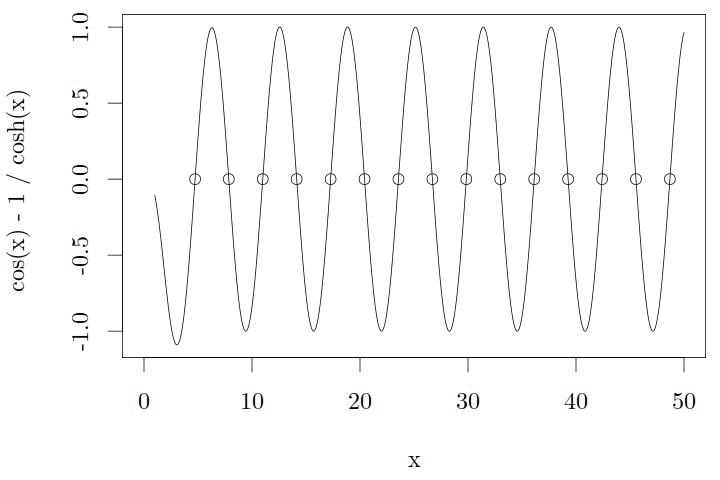
\includegraphics[width=\textwidth]{figures/eq_roots.png}
        \caption{Equation \ref{eq:roots} and its solutions.}
        \label{subfig:roots}
    \end{subfigure}
    ~
    \begin{subfigure}[b]{0.48\textwidth}
        \centering
        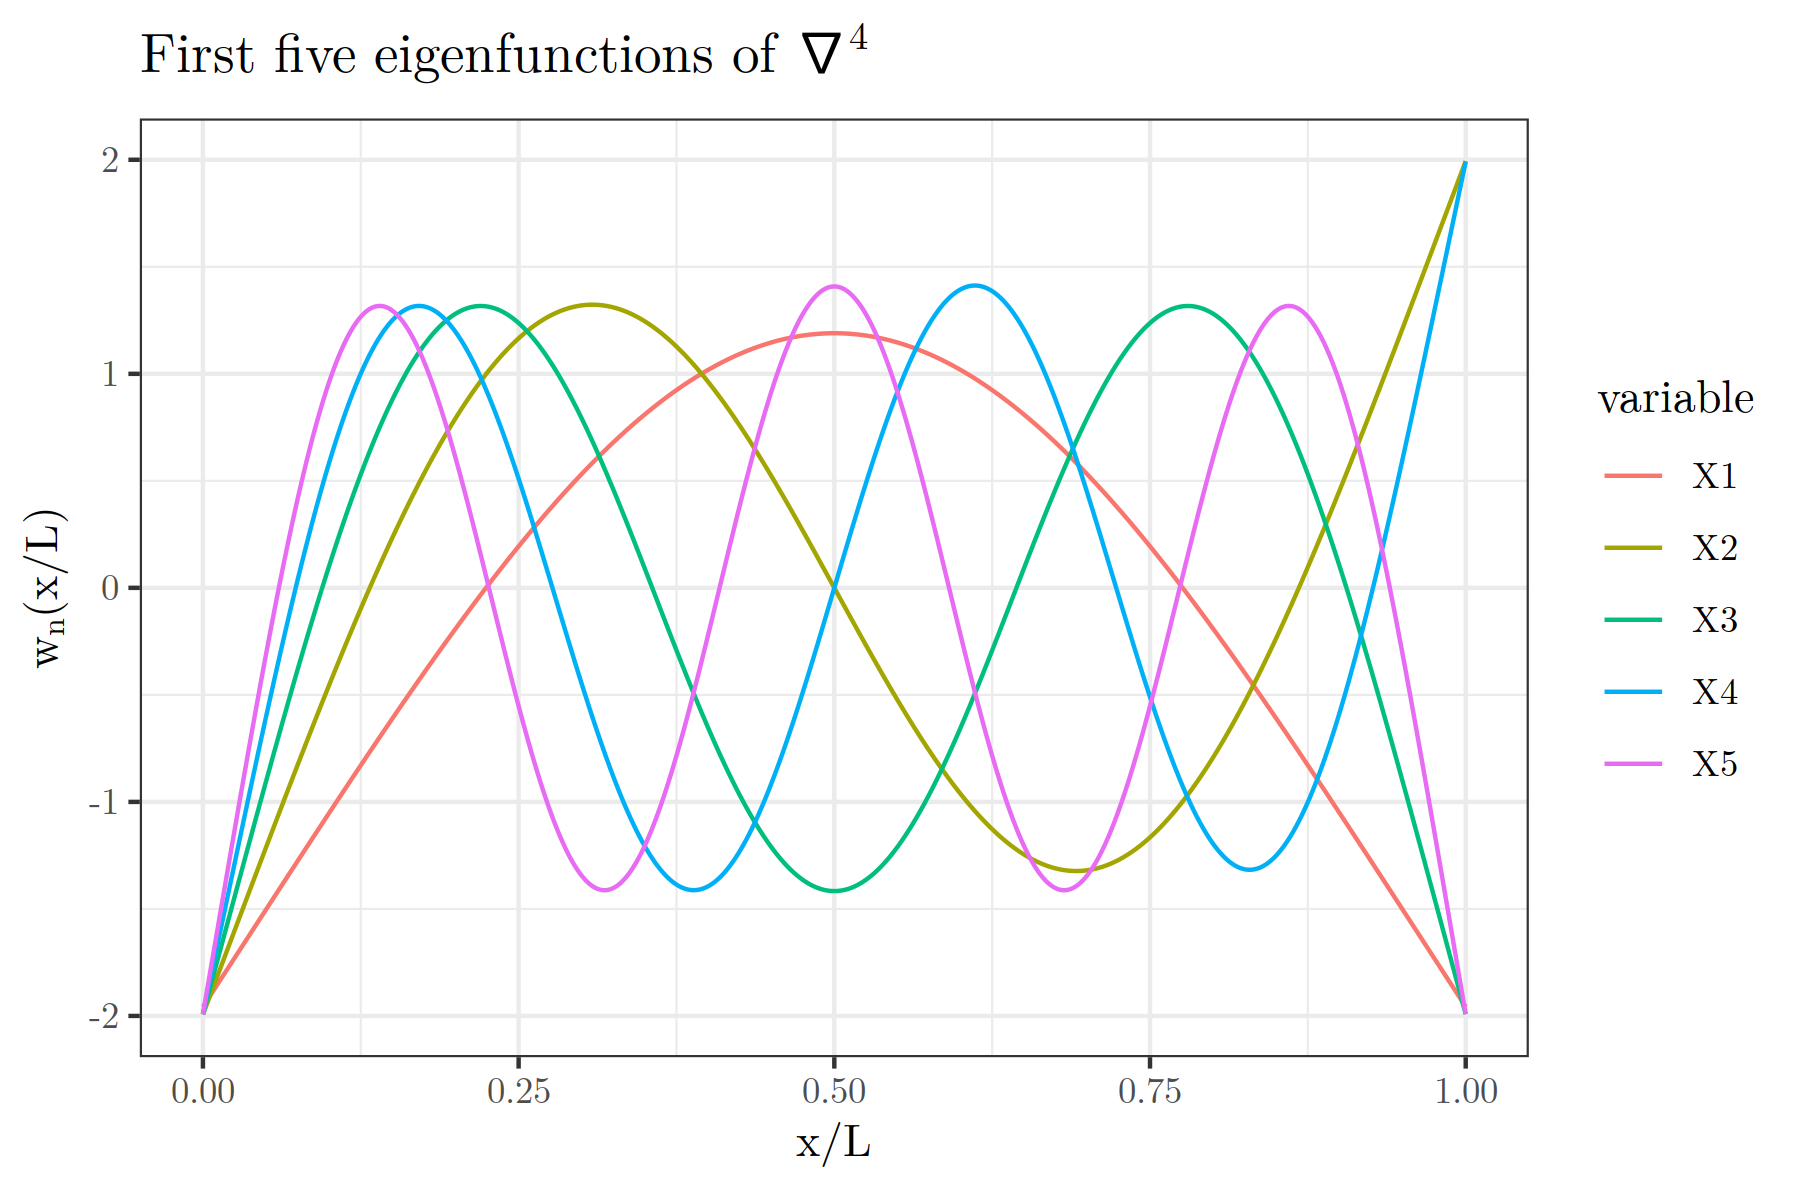
\includegraphics[width=\textwidth]{figures/efuncs.png}
        \caption{The first five eigenfunctions $f_n$ of boundary value problem \ref{eq:bvp}.}
        \label{subfig:efuncs}
    \end{subfigure}
    \caption{Solving the boundary value problem in equation \ref{eq:bvp}}
    \label{fig:bvp_sol}
\end{figure}

Letting $f(x) = \sum_{n=1}^\infty a_n f_n(x)$, we get that $a_n = \int_0^1 g(x, 0) f_n(x)dx$, and the complete dynamics of the height function are given by 

\begin{align}
    h(x, t) &= h_*(x) + g(x) = h_*(x) + \sum_{n=1}^\infty a_n e^{k_n^4 t} f_n(x). \label{eq:sol}
\end{align}

\noindent In practice, only the solutions $k_n$ to equation \ref{eq:roots} shown in Figure \ref{subfig:roots} are used, since the approximation to $h(x, 0)$ is close and higher $k_n$ result in precision errors when calculating $\cosh kx$ and $\sinh kx$. 

For the initial conditions given previously, the time evolution of $h(x, t)$ is shown in Figure \ref{fig:shapes}. We can make a few observations:

\begin{itemize}
    \item The system evolves extremely quickly in non-dimensional time. This is because each mode's evolution is given by rate $k_n^4$, which grows rapidly and makes higher order terms negligible almost immediately. Maybe it is worth asking what the values of the bending modulus and drag coefficient are to see if the timescale $\zeta L^4 / A$ is very large to compensate.
    \item The time evolution slows at larger $t$. This makes sense as the change in energy $\delta \varepsilon$ becomes smaller in magnitude when the curvature $h_{xx}(x, t)$ becomes closer to that of $h_*(x, t)$.
    \item We see some ``rolling inward'' of the change in curvature from the outer edge, most clearly at $t = \num{9e-4}$. However, it does not seem as pronounced as in \textit{C. flexa} inversion, at least not to me. When the organism inverts, it seems to have a wave of flipping that moves from the edge towards the center. Perhaps this is because the \textit{C. flexa} collars are stiff such that they resist compression or stretching in the sheet. Our representation used here does not penalize the filament compressing, which it clearly does as its arclength decreases substantially during the transition. 
\end{itemize}

\begin{figure}[bthp]
    \centering
    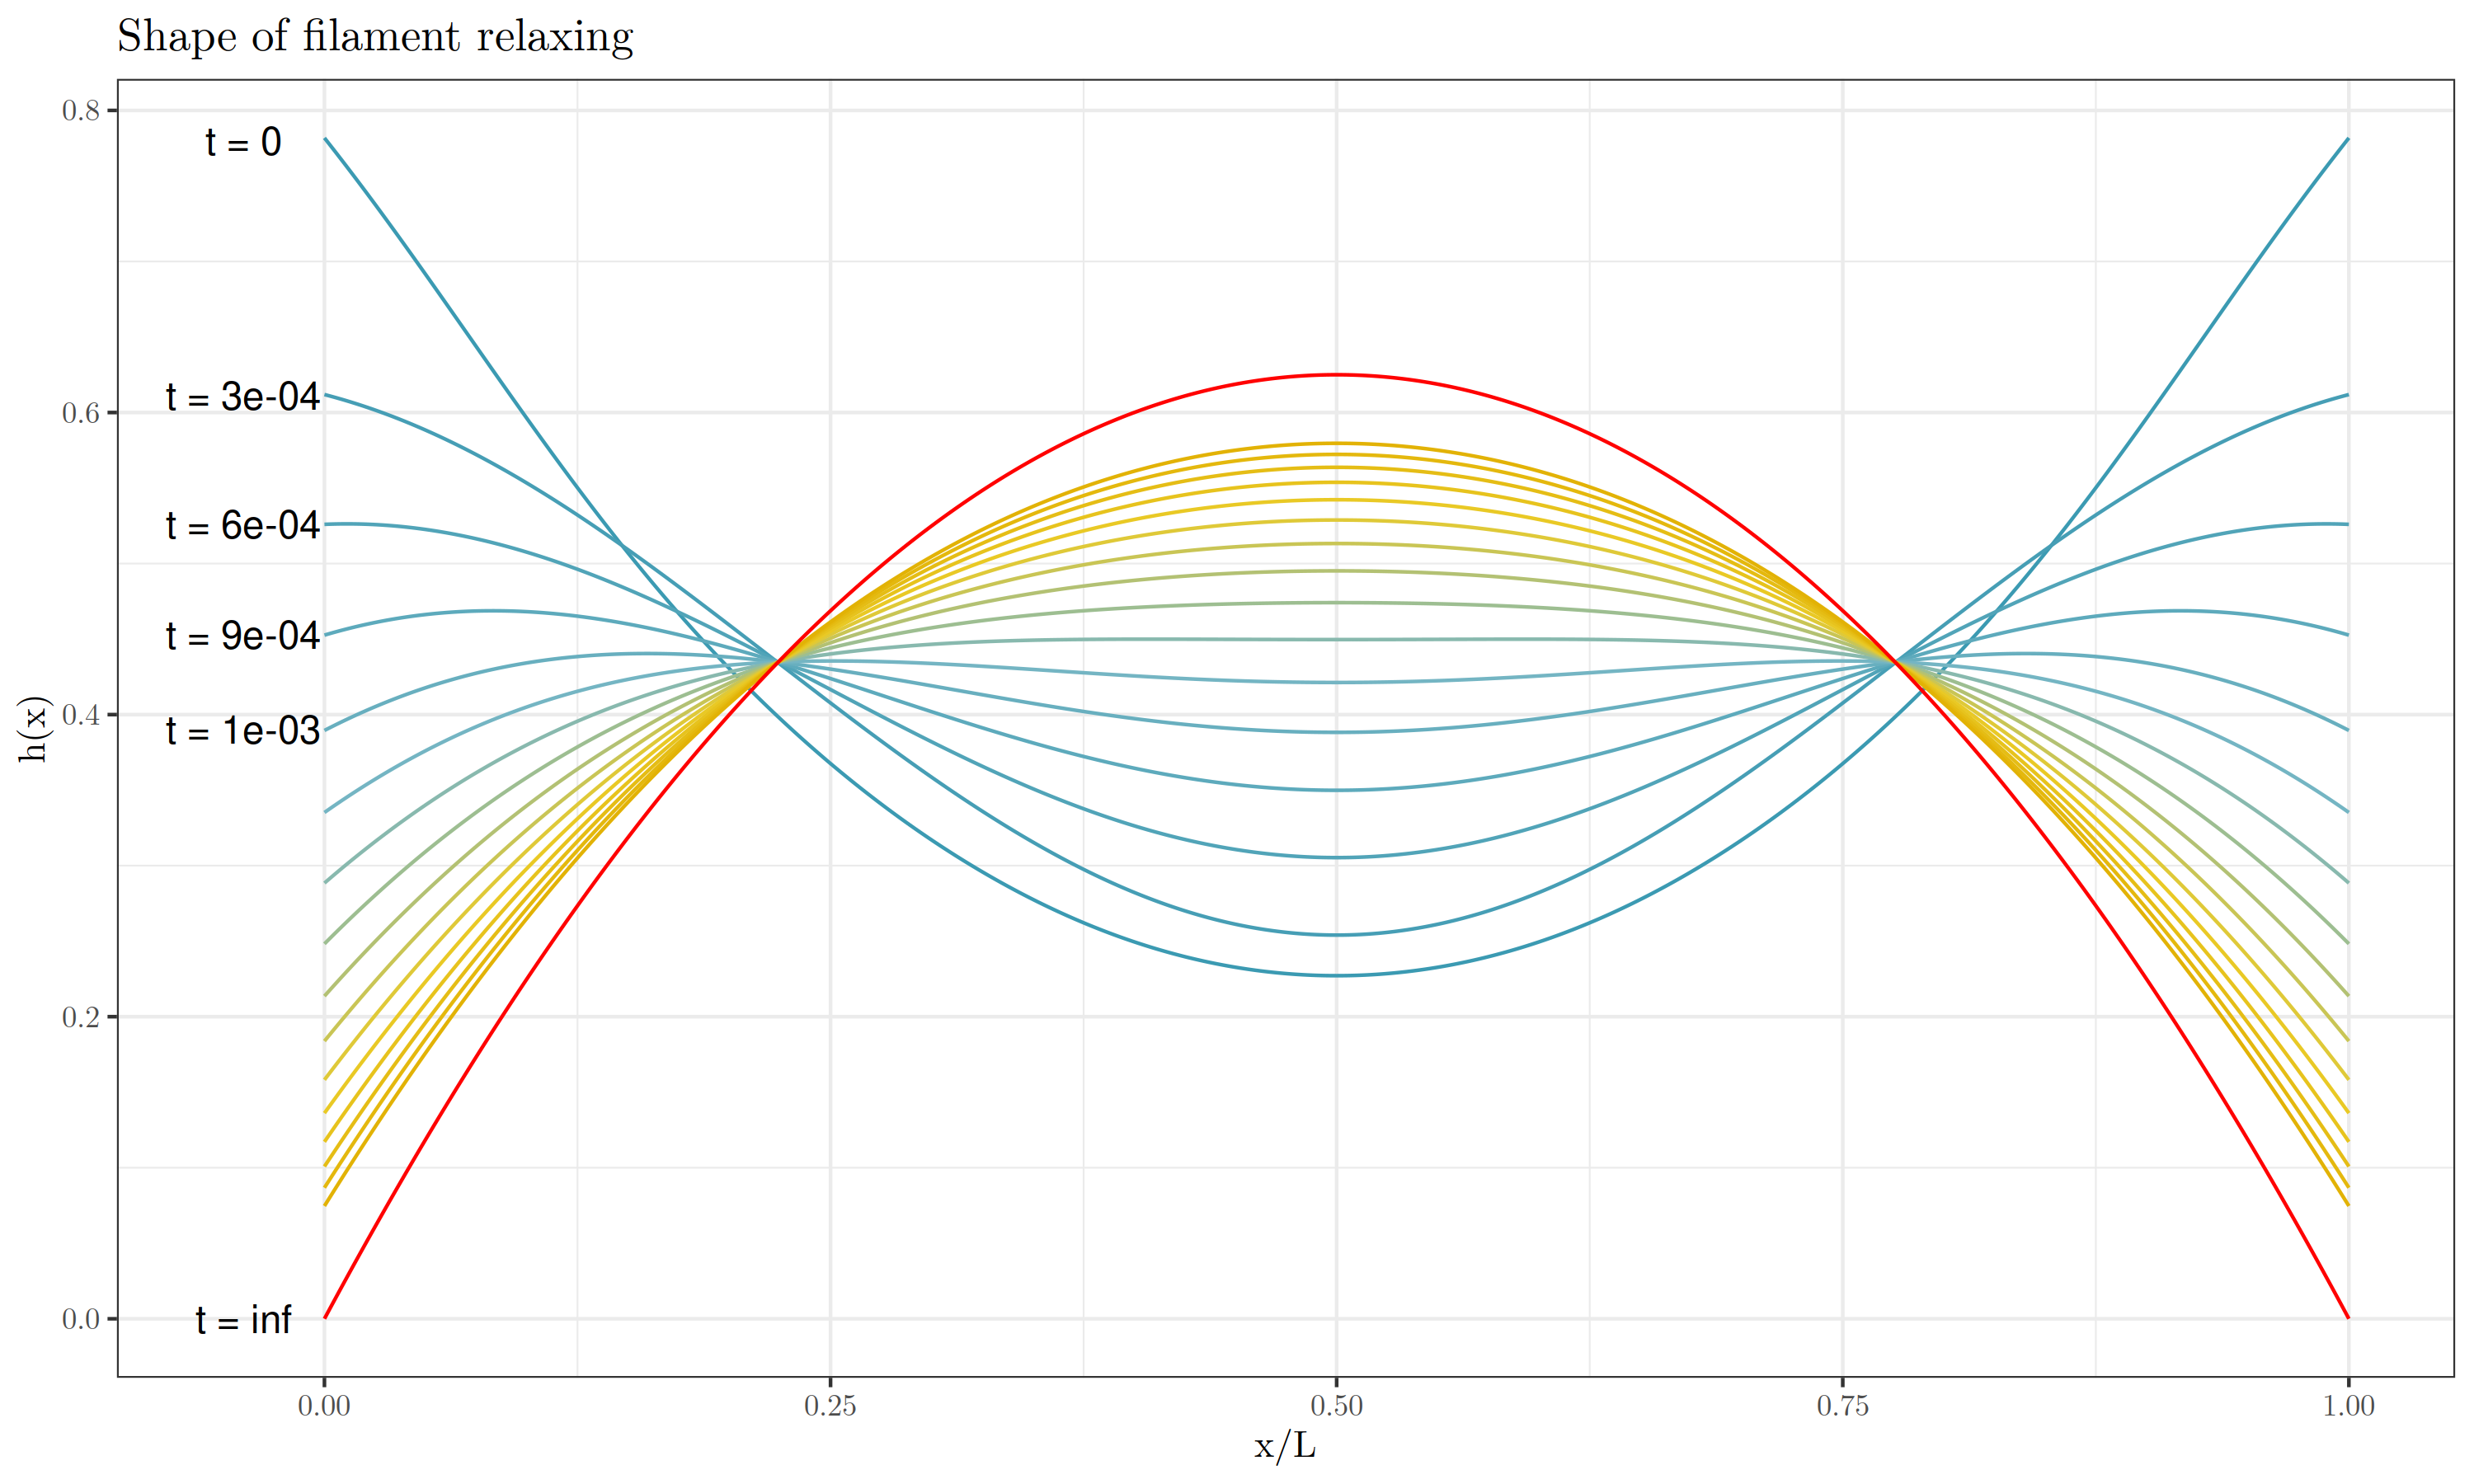
\includegraphics[width=\textwidth]{figures/shapes.png}
    \caption{Time evolution of a one-dimensional filament which switches prescribed curvature sign instantaneously. Time and length are given in dimensionless units defined by the length $L$, bending modulus $A$, and drag coefficient $\zeta$. The time unlabeled time intervals continue sequentially in intervals of $\Delta t = \num{3e-4}$.}
    \label{fig:shapes}
\end{figure}

\newpage 

\section{Expanded model}

The simplified dynamics that we get from the Mange representation lack energetic costs from the compression and extension that come with deforming a two dimensional surface. The logical step to include these energies is to model the flexa sheet a surface of revolution based on a curve $\bm{r}(\rho, \theta)=(\rho \cos \theta, \rho \sin \theta, z(\rho))$ with cylindrical coordinates $\rho, \theta$ and height function $z$. In doing so, we could take the elastohydrodynamic equation of motion written in terms of curvature $H$ and $K$ and express it as purely as a function of $z$.

We will proceed by writing the equations of motion generally for a surface and reducing it to a surface of revolution.

\subsection{$H$ and collar connection angle}

Before getting into the continuous sheet problem, it is worth describing the two degrees of freedom that our collar connections afford. The collar makes an angle $\phi$ between the vector pointing directly out of the cell and the vector between the cell and its collar boundary with the next cell. Additionally, there is an angle between the collars of two adjacent cells $\psi$. The latter results in the sheet's curvature, so we want to relate it to mean curvature $H$ or preferred curvature $H_0$. 

\begin{figure}[htbp]
    \centering
    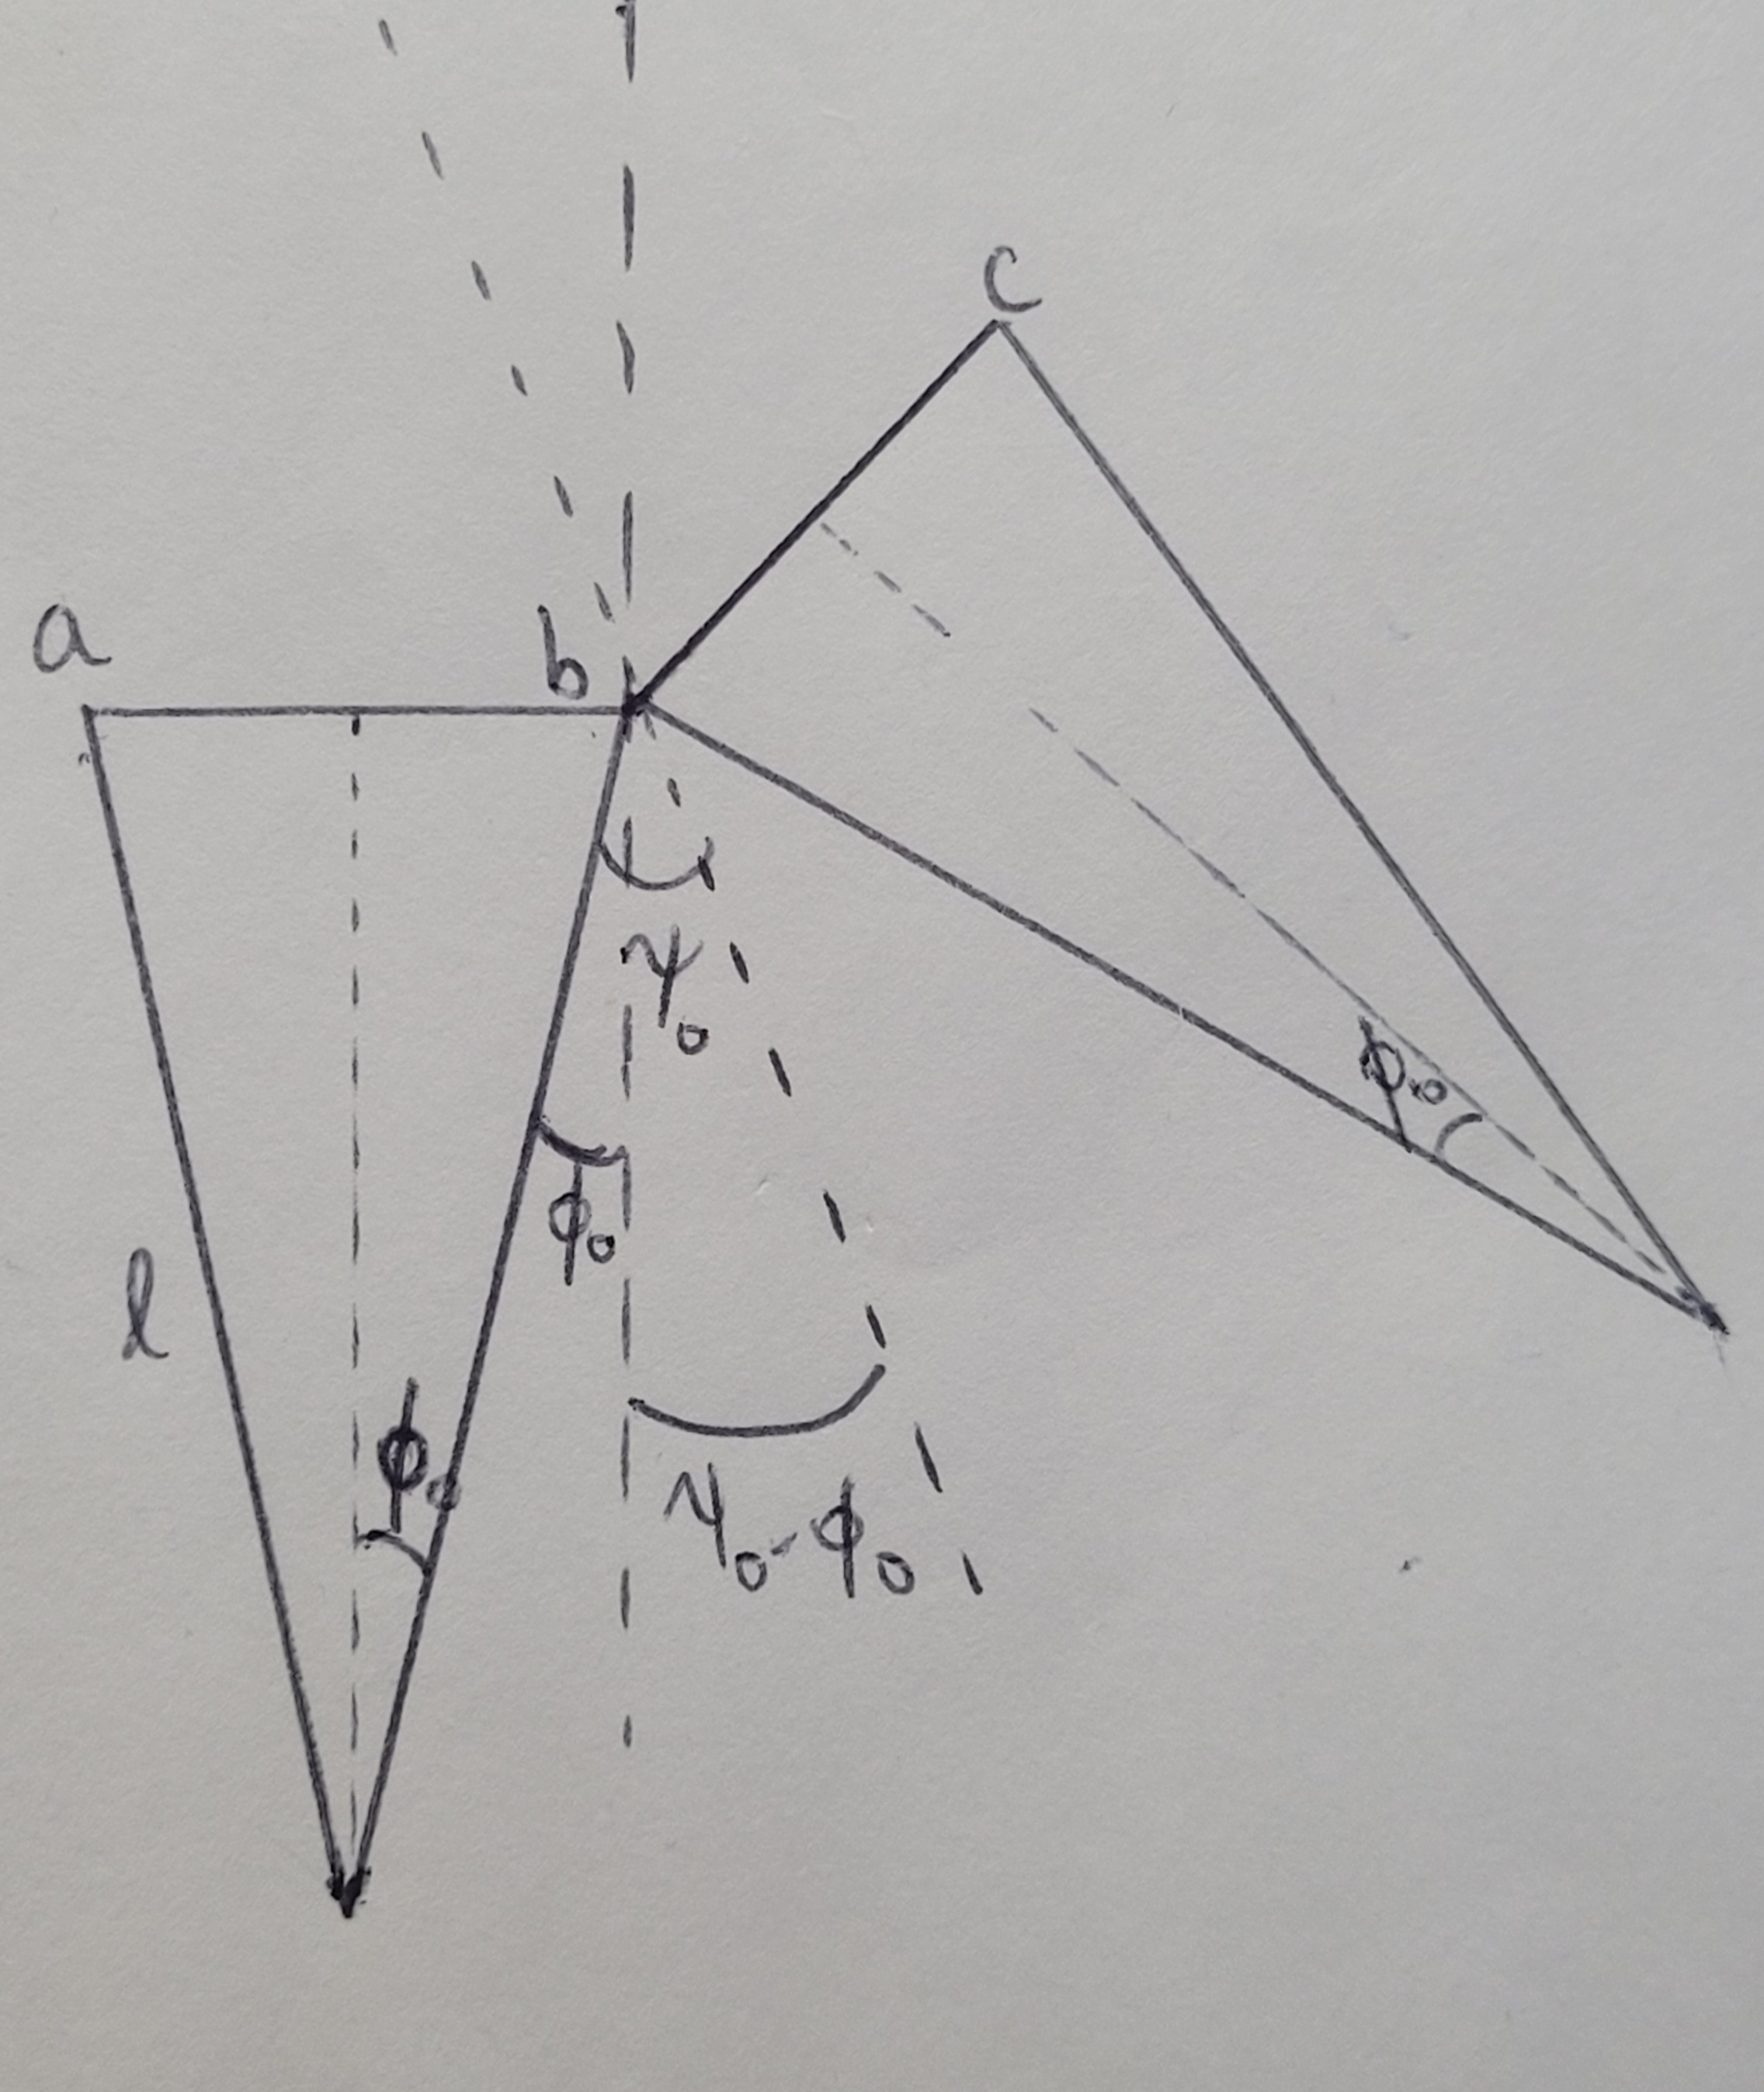
\includegraphics[width=0.5\textwidth]{figures/hpsi.jpg}
    \caption{Geometry for relating collar boundary angle $\psi$ to curvature $H$. }
    \label{fig:hpsi}
\end{figure}

Consider two neighboring cells with collar boundaries $a$, $b$, and $c$, as shown in Figure \ref{fig:hpsi}. We might imagine defining a radius of curvature by the circle that passes through the three collar boundaries. If we set $\bm{x_a} = 2\ell\sin\phi_0(-1, 0)$, $\bm{x_b} = (0,0)$, and $\bm{x_c} = 2\ell\sin\phi_0 (\sin(\psi_0 - \phi_0), \cos(\psi_0-\phi_0)$, we can solve for the circle coordinates 

\begin{align*}
    (x_\circ, y_\circ) &= \ell \sin\phi_0\left(-1, \frac{1+\cos2(\psi_0 - \phi_0)}{\sin2(\psi_0 - \phi_0)} \right)
\end{align*}

\noindent to get the inverse radius of curvature 

\begin{align}
    H_0 = \frac{1}{\sqrt{x_\circ^2 + y_\circ^2}} &= \frac{\sin(\psi_0 - \phi_0)}{\ell \sin\phi_0}. 
\end{align}

This has a nice, simple interpretation in that if $\psi_0 > \phi_0$, $H_0 > 0$ (as drawn in Figure \ref{fig:hpsi}). On the other hand, $\psi_0 < \phi_0$ implies $H_0 < 0$, or the sheet is concave on the cell body side. 

Alternatively, we solve for $\psi_0$ as a function of $H_0$,

\begin{align}
    \psi_0 &= \phi_0 + \arcsin \left( H_0 \ell \sin \phi_0 \right). \label{eq:h0_psi}
\end{align}

As we find later in equation \ref{eq:hlb}, the curvature of the sheet in any given direction is greater than or equal to $-1/\ell$ (cell bodies and collars cannot go through each other). This lower bound corresponds in \ref{eq:h0_psi} to $\psi_0 = 0$, which we expect when cells are pressing tightly against each other (Figure \ref{fig:maxcurv}).


\subsection{Problem statement} \label{subsec:problem}

\textcite{powers2010} (Section IV.B) shows that for an energy density $\e$ written in terms of the first and second fundamental forms $g_{\alpha\beta}$ and $K_{\alpha\beta}$, we can write an expression for the stress tensor $\bm{F}^\alpha$ 

\begin{align}
    \bm{F}^\alpha &= \left(T^{\alpha\beta} + \e^{\alpha\beta}K_\gamma^\beta \right)\bm{t}_\beta - (\nabla_\beta \e^{\alpha\beta})\hat{\bm{n}}. \label{eq:stress}
\end{align}

\noindent Here, $K_\gamma^\beta = K_{\gamma \delta}g^{\delta \beta}$, $\bm{t}_\beta = \partial_\beta \bm{r}$, and 

\begin{align*}
    T^{\alpha\beta} &= g^{\alpha\beta} \e + 2 \frac{\partial \e}{\partial g_{\alpha\beta}} = \frac{2}{\sqrt{g}} \frac{\partial}{\partial g_{\alpha\beta}} \left(\sqrt{g}\e \right) \\
    \e^{\alpha\beta} &= \frac{\partial \e}{\partial K_{\alpha\beta}}
\end{align*}

\noindent with $g = \det{g_{\alpha\beta}}$.

Since the force $\bm{f}$ acting on a surface point is given by the covariant divergence of the stress $\nabla_\alpha \bm{F}^\alpha$, our problem is effectively solved once we decide on an appropriate energy density. \textcite{brunet2019} showed that the angle formed by the \textit{C. flexa} collars changes when individual cells are triggered for inversion. We might reasonably suggest preferred sheet curvature is prescribed by changing the preferred angle of the collar $\phi_0$ and imposing and energetic cost based on the amount that the collar angle $\phi(\theta)$ differs around the collar in $\theta$: $\e \sim \int (\phi(\theta) - \phi_0)^2 d\theta$.

\subsection{Connecting continuous surface with individual cell mechanics}

For any point on a smooth surface, we could find an orthonormal basis of eigenvectors $\bm{e}_1, \bm{e}_2$ in the tangent space that diagonalises $K_\mu^\nu$. In terms of a vector $\bm{\Delta \xi}$ written in this basis, we have that the change in height with respect to the tangent plane and its normal $\Delta h$ is given by $K_{\mu\nu}\Delta\xi^\mu\Delta\xi^\nu$.

Let's consider a cell with collar angle $\phi(\theta)$, where $\theta$ measures the location on the collar. If the cell has an optimal collar angle $\phi_0$ and corresponding optimal curvature $K_{0\mu\nu}$, then the height of the collar will be $K_{0\mu\nu}\Delta\xi_0^\mu\Delta\xi_0^\nu$. The distance from the centerline of the cell (the norm of $\bm{\Delta\xi_0}$) is determined by $\phi_0$. The geometry is shown in Figure \ref{fig:geom}.

\begin{figure}[htbp]
    \centering
    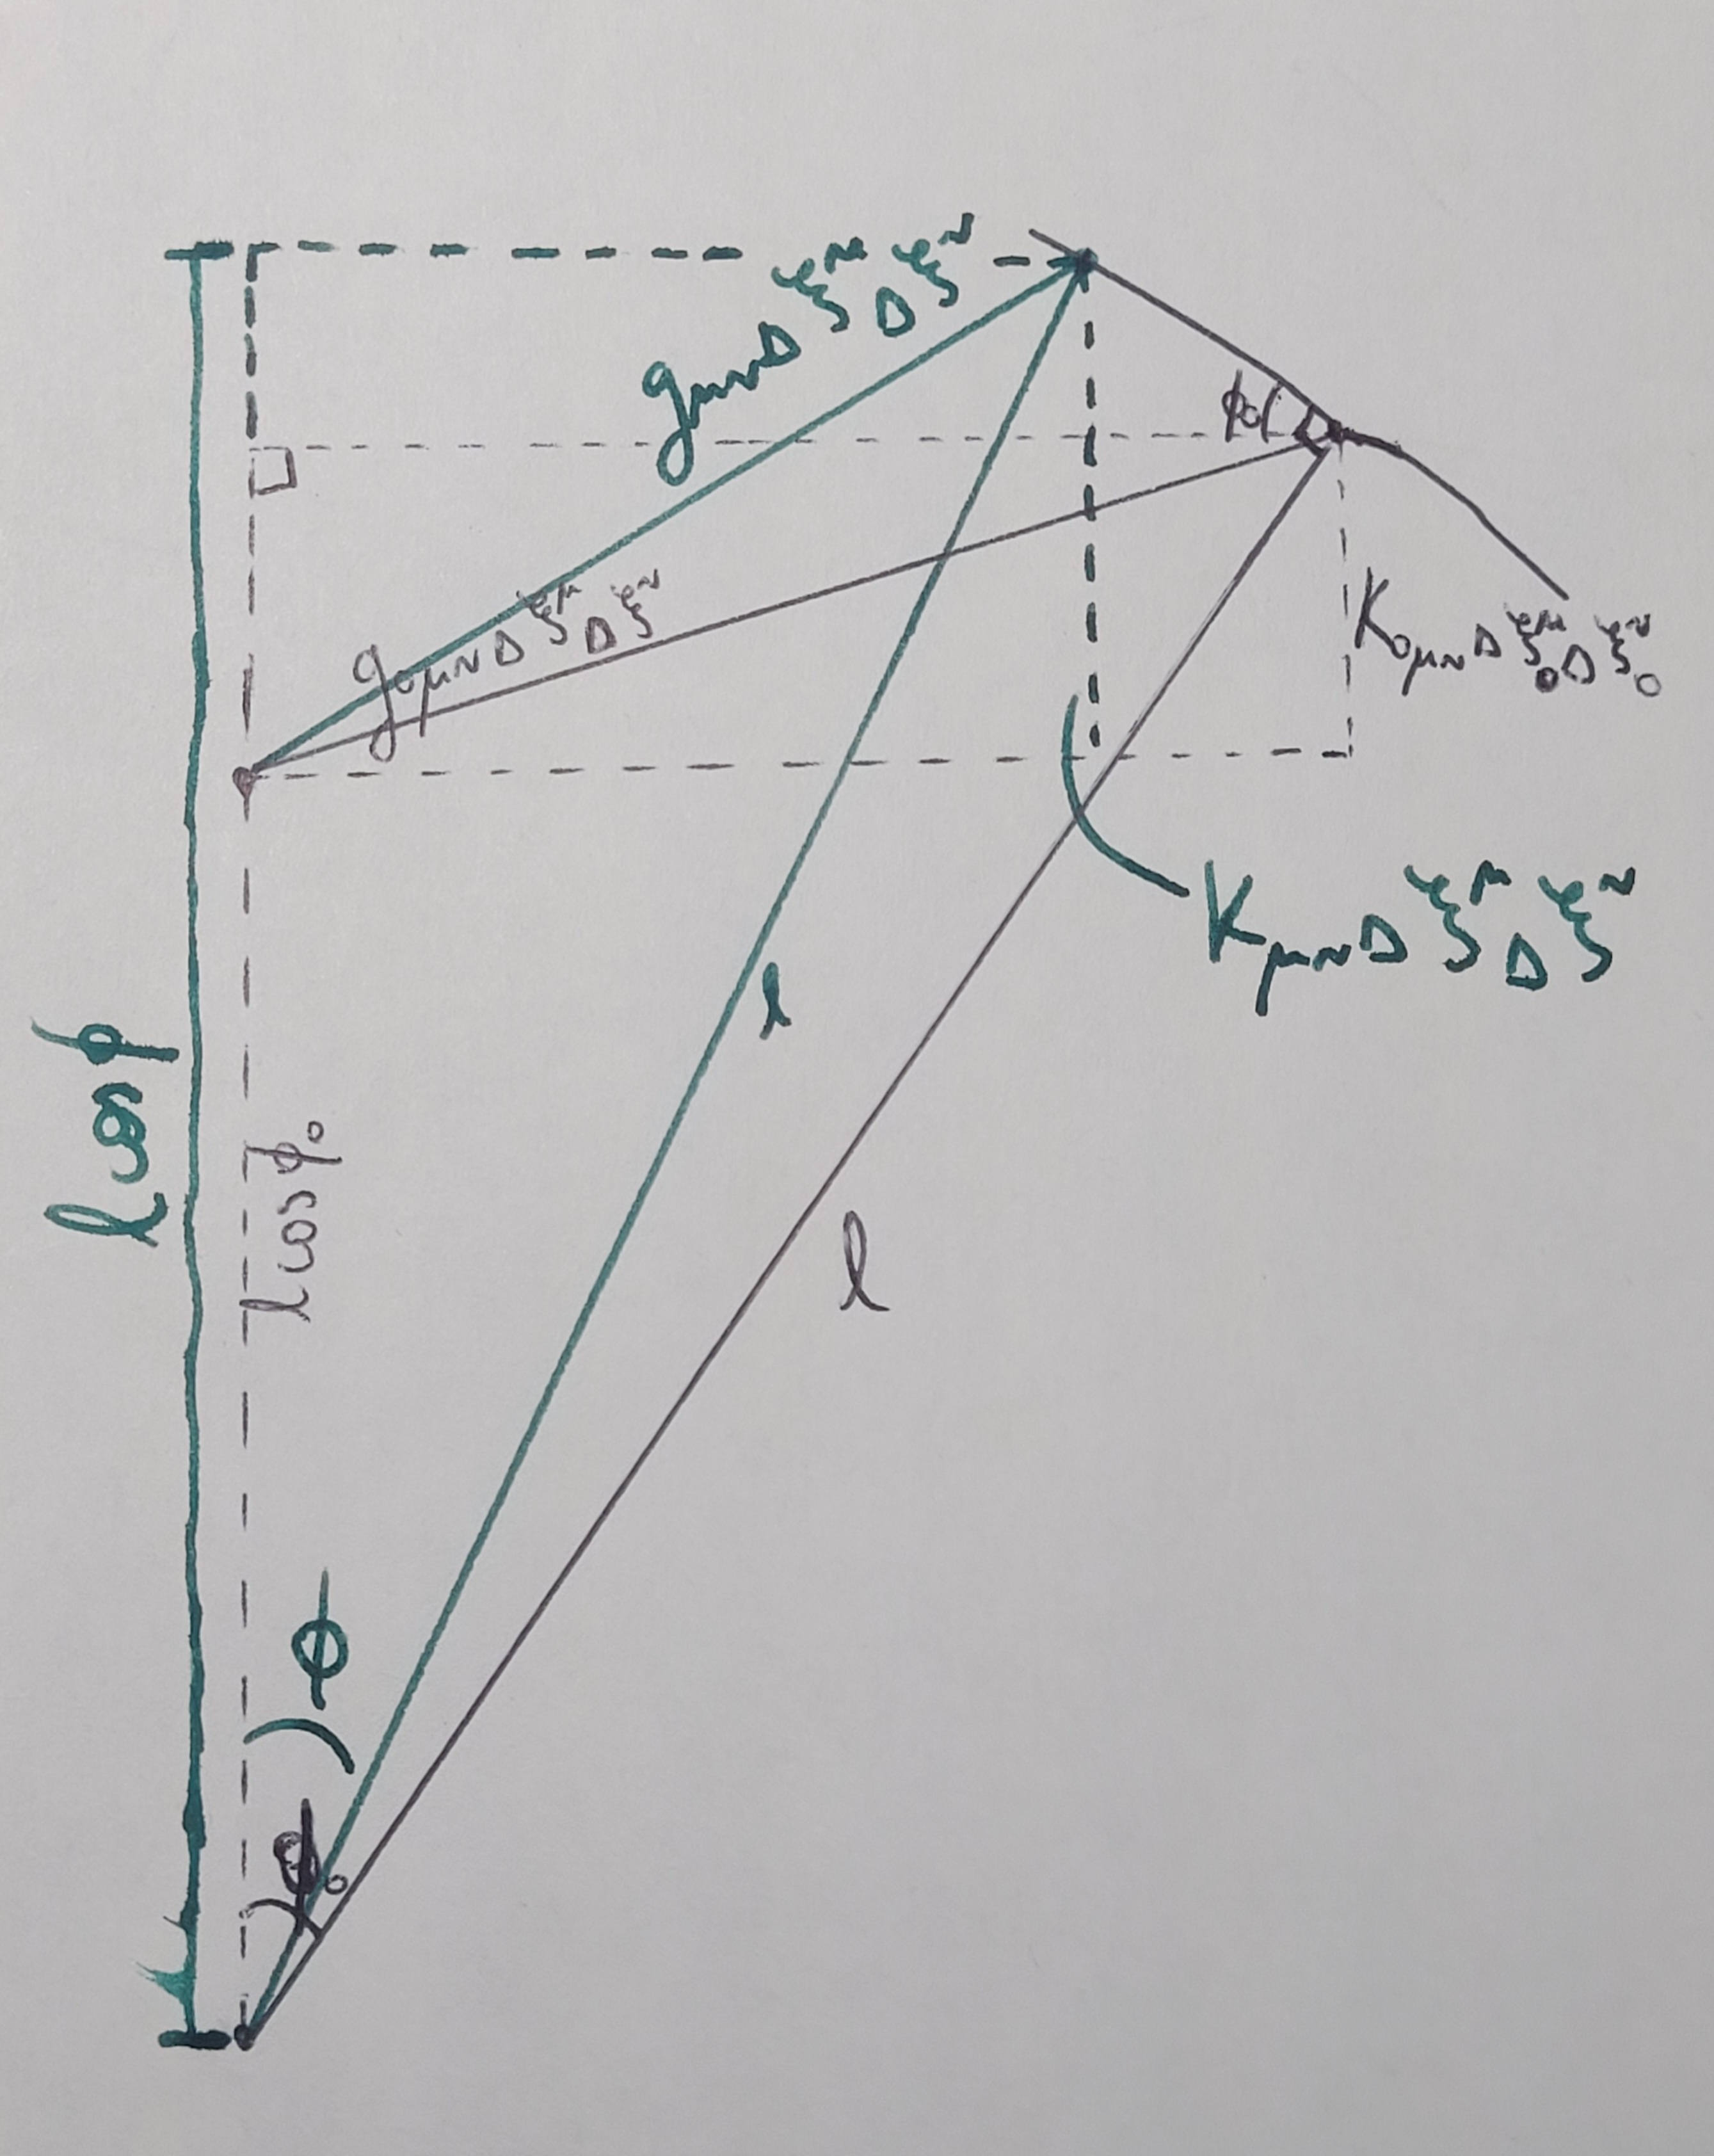
\includegraphics[width=0.75\textwidth]{figures/geom.jpg}
    \caption{Geometry of a single cell and collar with a continuous surface approximating the interactions between collars.}
    \label{fig:geom}
\end{figure}

If the cell has collar angle $\phi$ in direction $\theta$, we know the collar distance as $\bm{\Delta\xi} = \ell(\cos\phi, \sin\phi)$. For a fixed collar length $\ell$, we know the difference in height between the ground state and deformed state is $\ell(\cos\phi - \cos\phi_0)$. We can then relate the collar angle and sheet curvature by equating 

\begin{align}
    K_{\mu\nu}\Delta\xi^\mu\Delta\xi^\nu - K_{0\mu\nu}\Delta\xi_0^\mu\Delta\xi_0^\nu &= \ell(\cos\phi - \cos\phi_0). \label{eq:base}
\end{align}

The radius out from the center for the ground state is $\ell\sin\phi_0$ while for the deformed state it is $\ell\sin\phi$, so for $K_{011}=K_{022}=H_0$, we get

\begin{align*}
    K_{\mu\nu}\ell^2\sin^2\phi (\cos\theta, \sin\theta)^{\mu,\nu} - H_0 \ell^2\sin^2\phi_0 &= \ell(\cos\phi - \cos\phi_0) \\
    H_\theta \ell^2\sin^2\phi - H_0 \ell^2\sin^2\phi_0 &= \ell(\cos\phi - \cos\phi_0)
\end{align*}

\noindent where $H_\theta = K_{11}\cos^2\theta + K_{22}\sin^2\theta + 2K_{12}\sin\theta\cos\theta$ is the curvature of a line on the surface in direction $\theta$. We can cancel a factor of $\ell$, redefine units of length in terms of $\ell$ (such that $H_\theta$ is the ratio of $\ell$ with the radius of curvature in direction $\theta$), and express $\sin^2\phi$ in terms of $\cos\phi$ to get

\begin{align*}
    0 &= H_\theta \cos^2\phi + \cos\phi + (H_0\sin^2\phi_0 - \cos\phi_0 - H_\theta) \\
    \cos\phi &= \frac{-1 \pm \sqrt{1 + 4H_\theta (H_\theta + \cos\phi_0 - H_0\sin^2\phi_0)}}{2H_\theta}.
\end{align*}

If we take the collars to always have angle $0 \leq \phi \leq \pi/2$, we can constrain $0 \leq \cos\phi \leq 1$ to find the two inequalities 

\begin{align}
    H_\theta \geq H_0 \sin^2\phi_0 - \cos\phi_0 \label{eq:ineq1}\\
    1 \geq \cos\phi_0 - H_0 \sin^2\phi_0. \label{eq:ineq2}
\end{align}

\noindent The second inequality can be simplified to $H_0 \geq -(1+\cos\phi_0)^{-1}$. Combining the two inequalities yields 

\begin{align}
    H_\theta \geq -1. \label{eq:hlb}
\end{align}

\noindent Re-expressed with units, this means that $H_\theta \geq -1/\ell$, or that the radius of curvature can never be smaller than $\ell$ on the cells' side. In other words, the cells can't push through each other! (Figure \ref{fig:maxcurv})

\begin{figure}[hbtp]
    \centering
    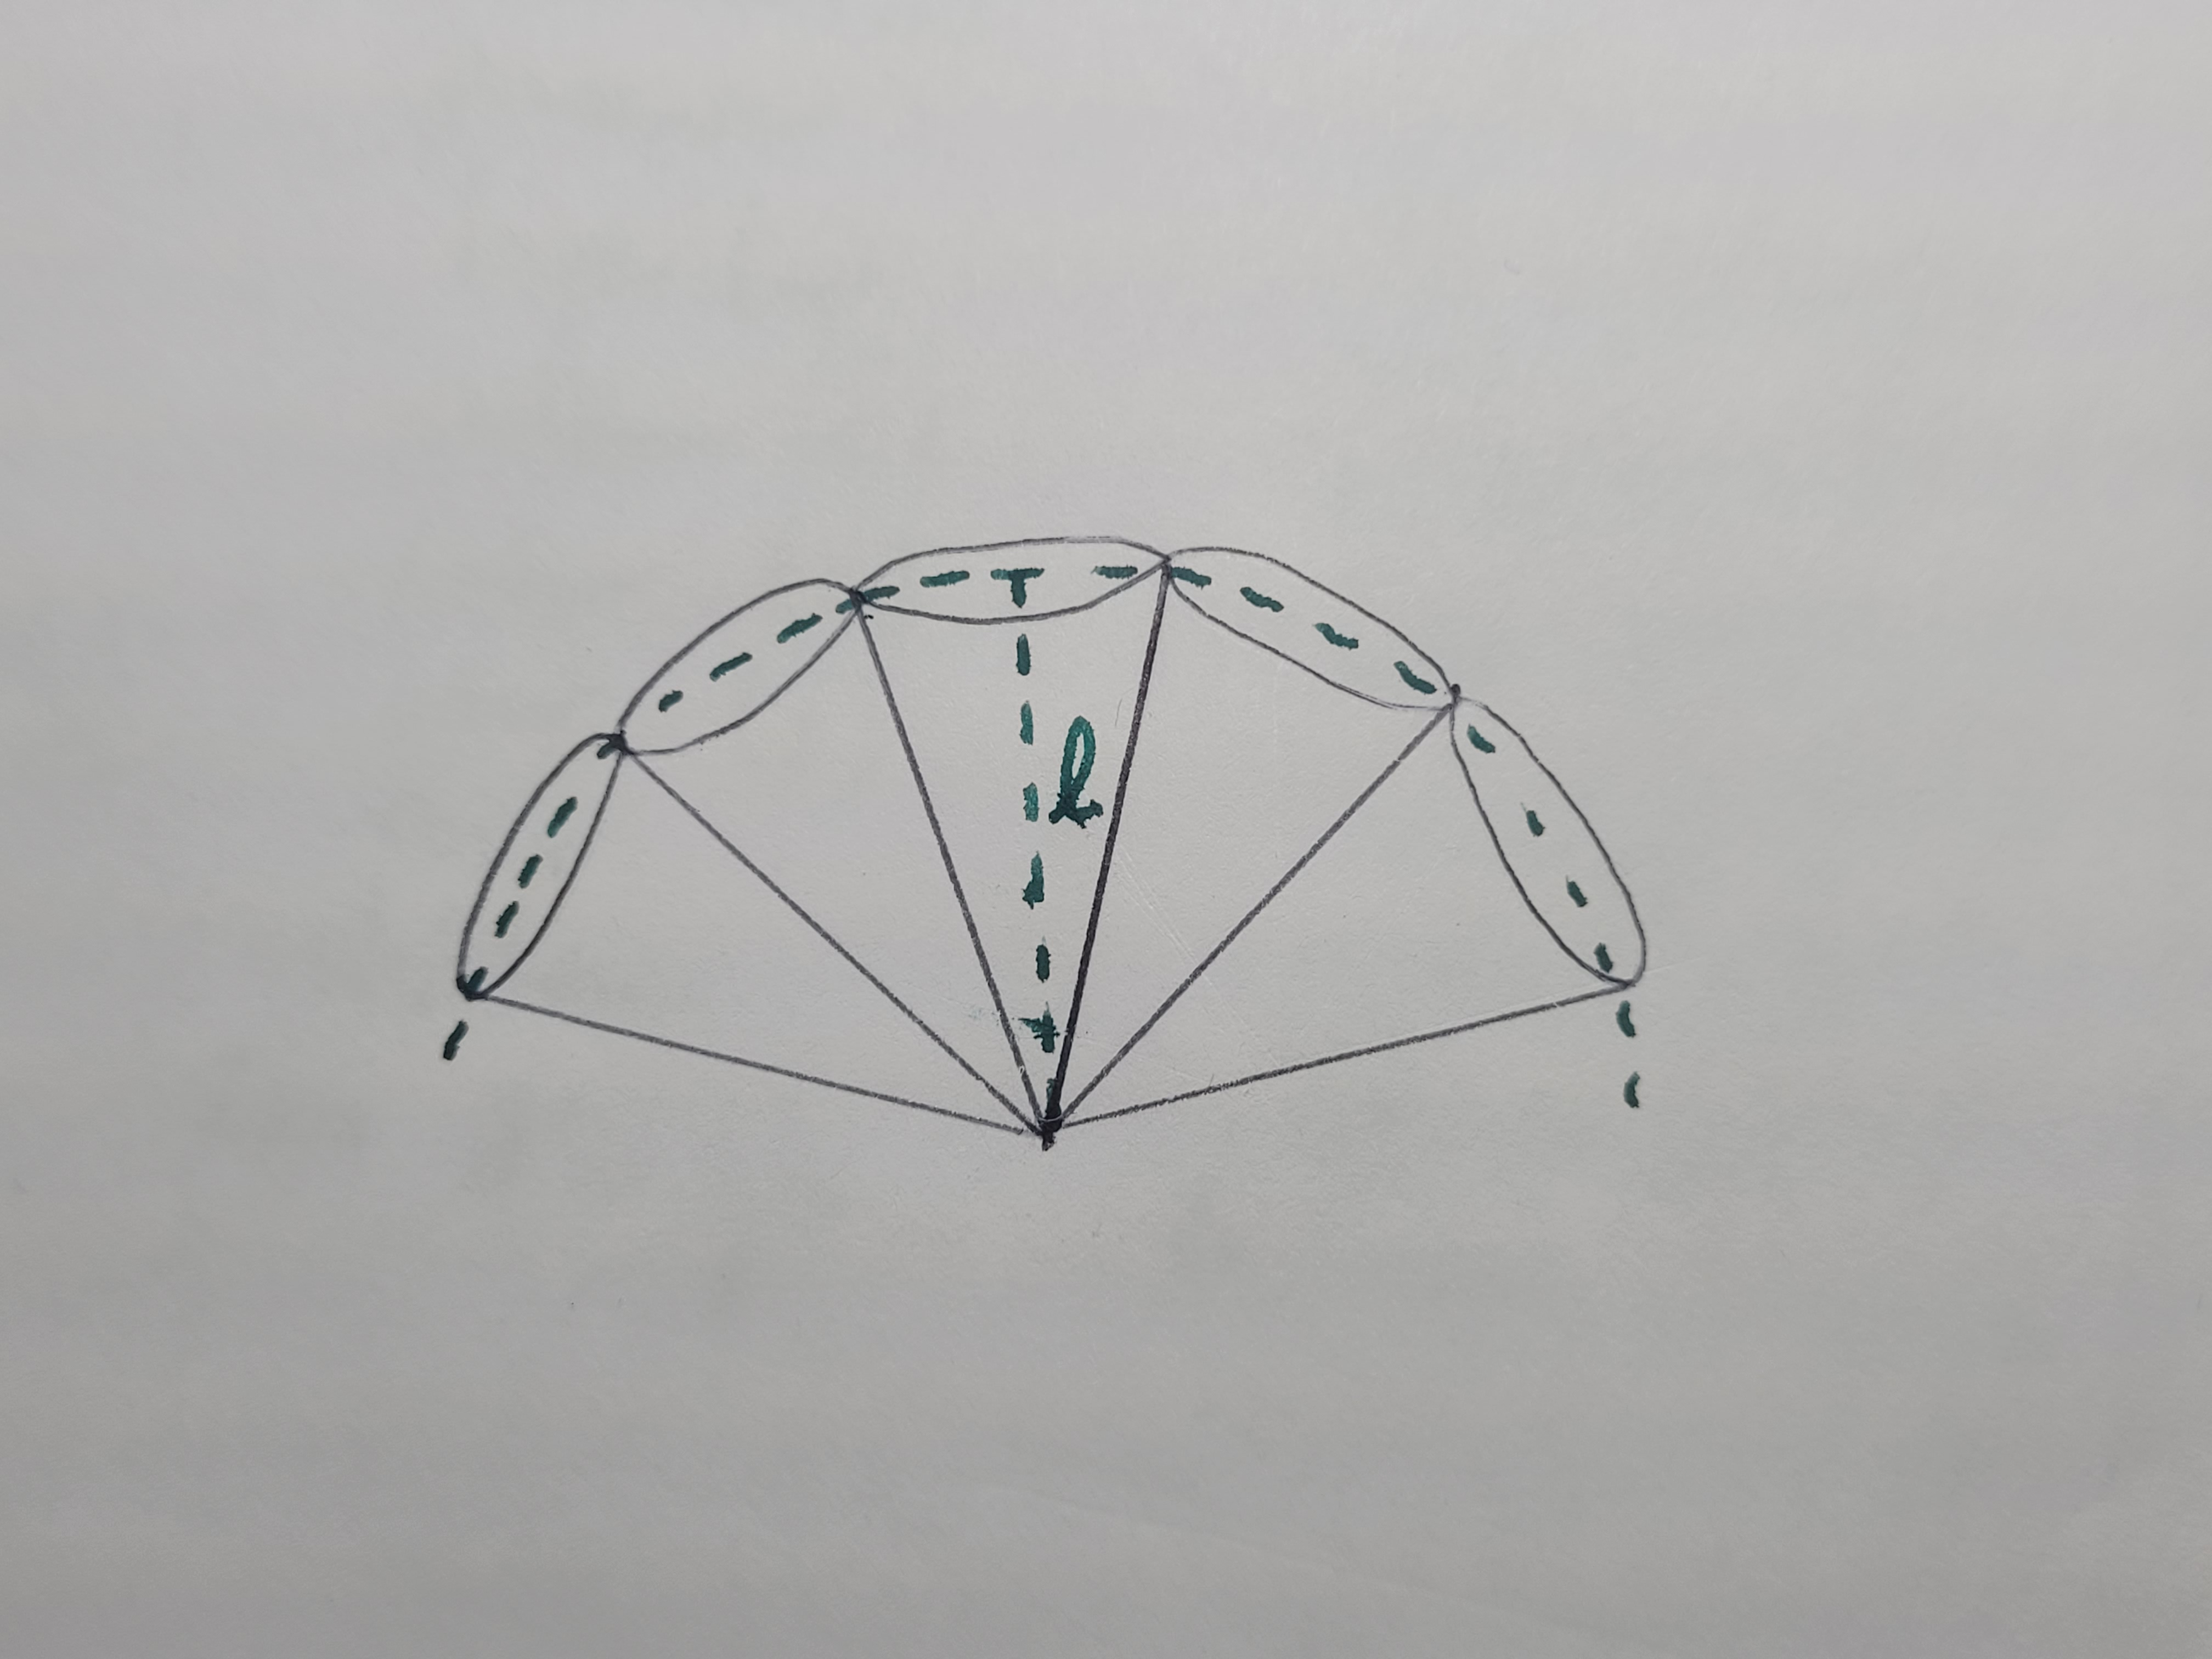
\includegraphics[width=0.5\textwidth]{figures/arc.jpg}
    \caption{Maximum cell-side curvature is given by inequalities \ref{eq:ineq1}, \ref{eq:ineq2} to have radius $\ell$. This corresponds to every (point) cell bumping into each other.}
    \label{fig:maxcurv}
\end{figure}

\subsection{Writing the energy}

We want to write equation \ref{eq:base} in terms of $\phi-\phi_0$ to write down the energy. We can use a trigonometric identity to write

\begin{align}
    H_\theta \sin^2\phi - H_0 \sin^2\phi_0 &= -2 \sin \frac{\phi - \phi_0}{2} \sin\frac{\phi + \phi_0}{2}. \label{eq:preapprox}
\end{align}

\noindent If $phi - phi_0$ is small in magnitude, then 

\begin{align*}
    \sin\frac{\phi - \phi_0}{2} &\approx \frac{\phi - \phi_0}{2} \\
    \sin\frac{\phi + \phi_0}{2} = \sin\left(\phi_0 + \frac{\phi + \phi_0}{2} \right) &\approx \sin\phi_0 + \frac{\phi - \phi_0}{2} \cos\phi_0 \\
    \sin^2\phi = \sin^2\left(\phi_0 + (\phi - \phi_0) \right) &\approx \sin^2\phi_0 +(\phi - \phi_0)\sin2\phi_0.
\end{align*}

Using these approximations we rewrite equation \ref{eq:preapprox} to first order in $\phi - \phi_0$ as

\begin{align*}
    (H_\theta - H_0) \sin^2\phi_0 + H_\theta (\phi - \phi_0)\sin2\phi_0 &= -(\phi - \phi_0) \sin\phi_0 \\
    (H_\theta - H_0) \sin^2\phi_0 &= -(\phi-\phi_0) (H_\theta \sin2\phi_0 + \sin\phi_0) \\
    \frac{(H_\theta-H_0)^2 \sin^4\phi_0}{(H_\theta + \sin\phi_0 / \sin2\phi_0)^2 \sin^2 2\phi_0} &= (\phi - \phi_0)^2.
\end{align*}

We want to integrate this function in $\theta$, so let $K_{11} = a$, $K_{22} = b$, $K_{12} = c$, $-H_0 = d$ and $\sin\phi_0/ \sin 2 \phi_0 = e$ for simplicity when we write

\begin{align*}
    \int_{-\pi}^\pi (\phi - \phi_0)^2 d\theta &= \int_{-\pi}^\pi \frac{\left(a\cos^2\theta + b\sin^2\theta + 2c\sin\theta\cos\theta + d \right)^2}{\left(a\cos^2\theta + b\sin^2\theta + 2c\sin\theta\cos\theta + e \right)^2} d\theta \\
    &= \left\{-\sin2\theta \left[a^2 (-4bc\theta -4ce\theta + d^2 - 2de +e^2) + a(4b^2c\theta -2b(d-e)^2+4c\theta(c^2 - e^2)) \right. \right. \\
    &\qquad \qquad \qquad \left. + b^2(4ce\theta + d^2 -2de + e^2) + 4bc\theta(e^2 - c^2) + 4c^2 (d-e)^2 \right] \\
    &\qquad + 2(a + b +2e) \left[c^2 \theta (b - a) + \theta (a - b) (a + e) (b + e) - c (d - e)^2 \right] \\
    &\qquad \left.+ 2 \theta (a - b)^2 \cos(2 \theta) (a (b + e) + e (b + e) - c^2) \right\} \\
    &\qquad \big/ 2\left[(a - b) (a (b + e) + e (b + e) - c^2) ((a - b) \cos(2 \theta) + a + b + 2 c \sin(2 \theta) + 2 e)\right] \\
    &\quad + \frac{(e - d) (a (4 b + d + 3 e) + b d + 3 b e - 4 c^2 + 2 d e + 2 e^2) \tan^{-1}\left(\frac{-(b + e) \tan\theta - c}{\sqrt{a (b + e) + e (b + e) - c^2}}\right)}{2(a (b + e) + e (b + e) - c^2)^{3/2}}
\end{align*}

\noindent evaluated at $\theta = -\pi, \pi$. Evaluating this expression is surprisingly straightforward, and gives the result 

\begin{align*}
    \int_{-\pi}^\pi (\phi - \phi_0)^2 d\theta &= \text{const.} + \text{const.} \frac{4 K + 2(d+3e)H + 2de + e^2}{(K + 2H + e^2)^{3/2}}.
\end{align*}

Varying this expression will be more difficult than the typical membrane energy defined only in terms of curvature $(H-H_0)^2 + K$ since the Gaussian curvature term is not alone. This means that we cannot use the Gauss Bonnet theorem $\int_S K dA = 2\pi n + \oint_{\partial S}K ds$ to simply write it as a boundary term. Nevertheless, provided that we can vary $K$ on the surface, the shape equation that results shouldn't be very difficult to derive.

\subsection{Varying the energy}

Following subsection \ref{subsec:problem}, we just need to express our energy in terms of $K_{\mu\nu}$ and $g_{\mu\nu}$ to derive a force from it. We of course have that $H = (1/2) (K_{\mu\nu} g^{\mu\nu})$, which is easily differentiated with respect to $K_{\mu\nu}$ and $g_{\mu\nu}$. We can differentiate $K$ by re-expressing it with the identity $K^{\alpha\beta}K_{\alpha\beta} = 4H^2 - 2K$.\footnote{This comes from $4H^2 - 2K = (K^1_1 + K^2_2)^2 - 2(K^1_1K^2_2 - 2K^1_2) = (K^1_1)^2 + 2 K^1_2K^1_2 + (K^2_2)^2 = K^\alpha_\beta K_\alpha^\beta = K^{\alpha\beta}K_{\alpha\beta}$.} Then we have $K = (g^{\alpha\beta}K_{\alpha\beta})^2 - K_{\mu\nu}K_{\alpha\beta}g^{\mu\alpha}g^{\nu\beta}$.

\newpage
\section{Discrete surface model}
\subsection{How to define the surface}

We need to determine what parts of our physical problem we will keep track of, and how we will use them to define an energy. There are two natural, physical planar graphs to look at. We could either form the graph with cell bodies forming vertices and edges defined by cells whose collars make contact with each other. Alternatively, vertices could be represented by places where two cells' collars lose contact with each other, and edges could be along the line where those collars contact. 

Since these graphs are planar (albeit not necessarily lying along a physical plane), we have a well-defined notion of a graph dual, where each face in one graph corresponds to a vertex in the other. What we find is that the two graphs described above are dual to each other (Figure \ref{subfig:duals1}). One graph specifies the topology of the other, but we are considering these as spatial graphs to use their geometries so our problem is not so simple. Knowing the positions of all vertices and knowing the edges of one graph does not give complete information about the other.

Since each cell is identical, we might imagine that the distances between two cells and their mutual boundary is equal. In a loose sense, then, their interactions form a Voronoi tesselation on the surface of collar interactions (with respect to the metric on that surface). We can then take the dual to know that the graph of cell bodies is triangulated, as the dual of a Voronoi tesselation is a Delaunay triangulation (Figure \ref{subfig:duals2}).

\begin{figure}[htbp]
    \centering
    \begin{subfigure}[b]{0.52\textwidth}
        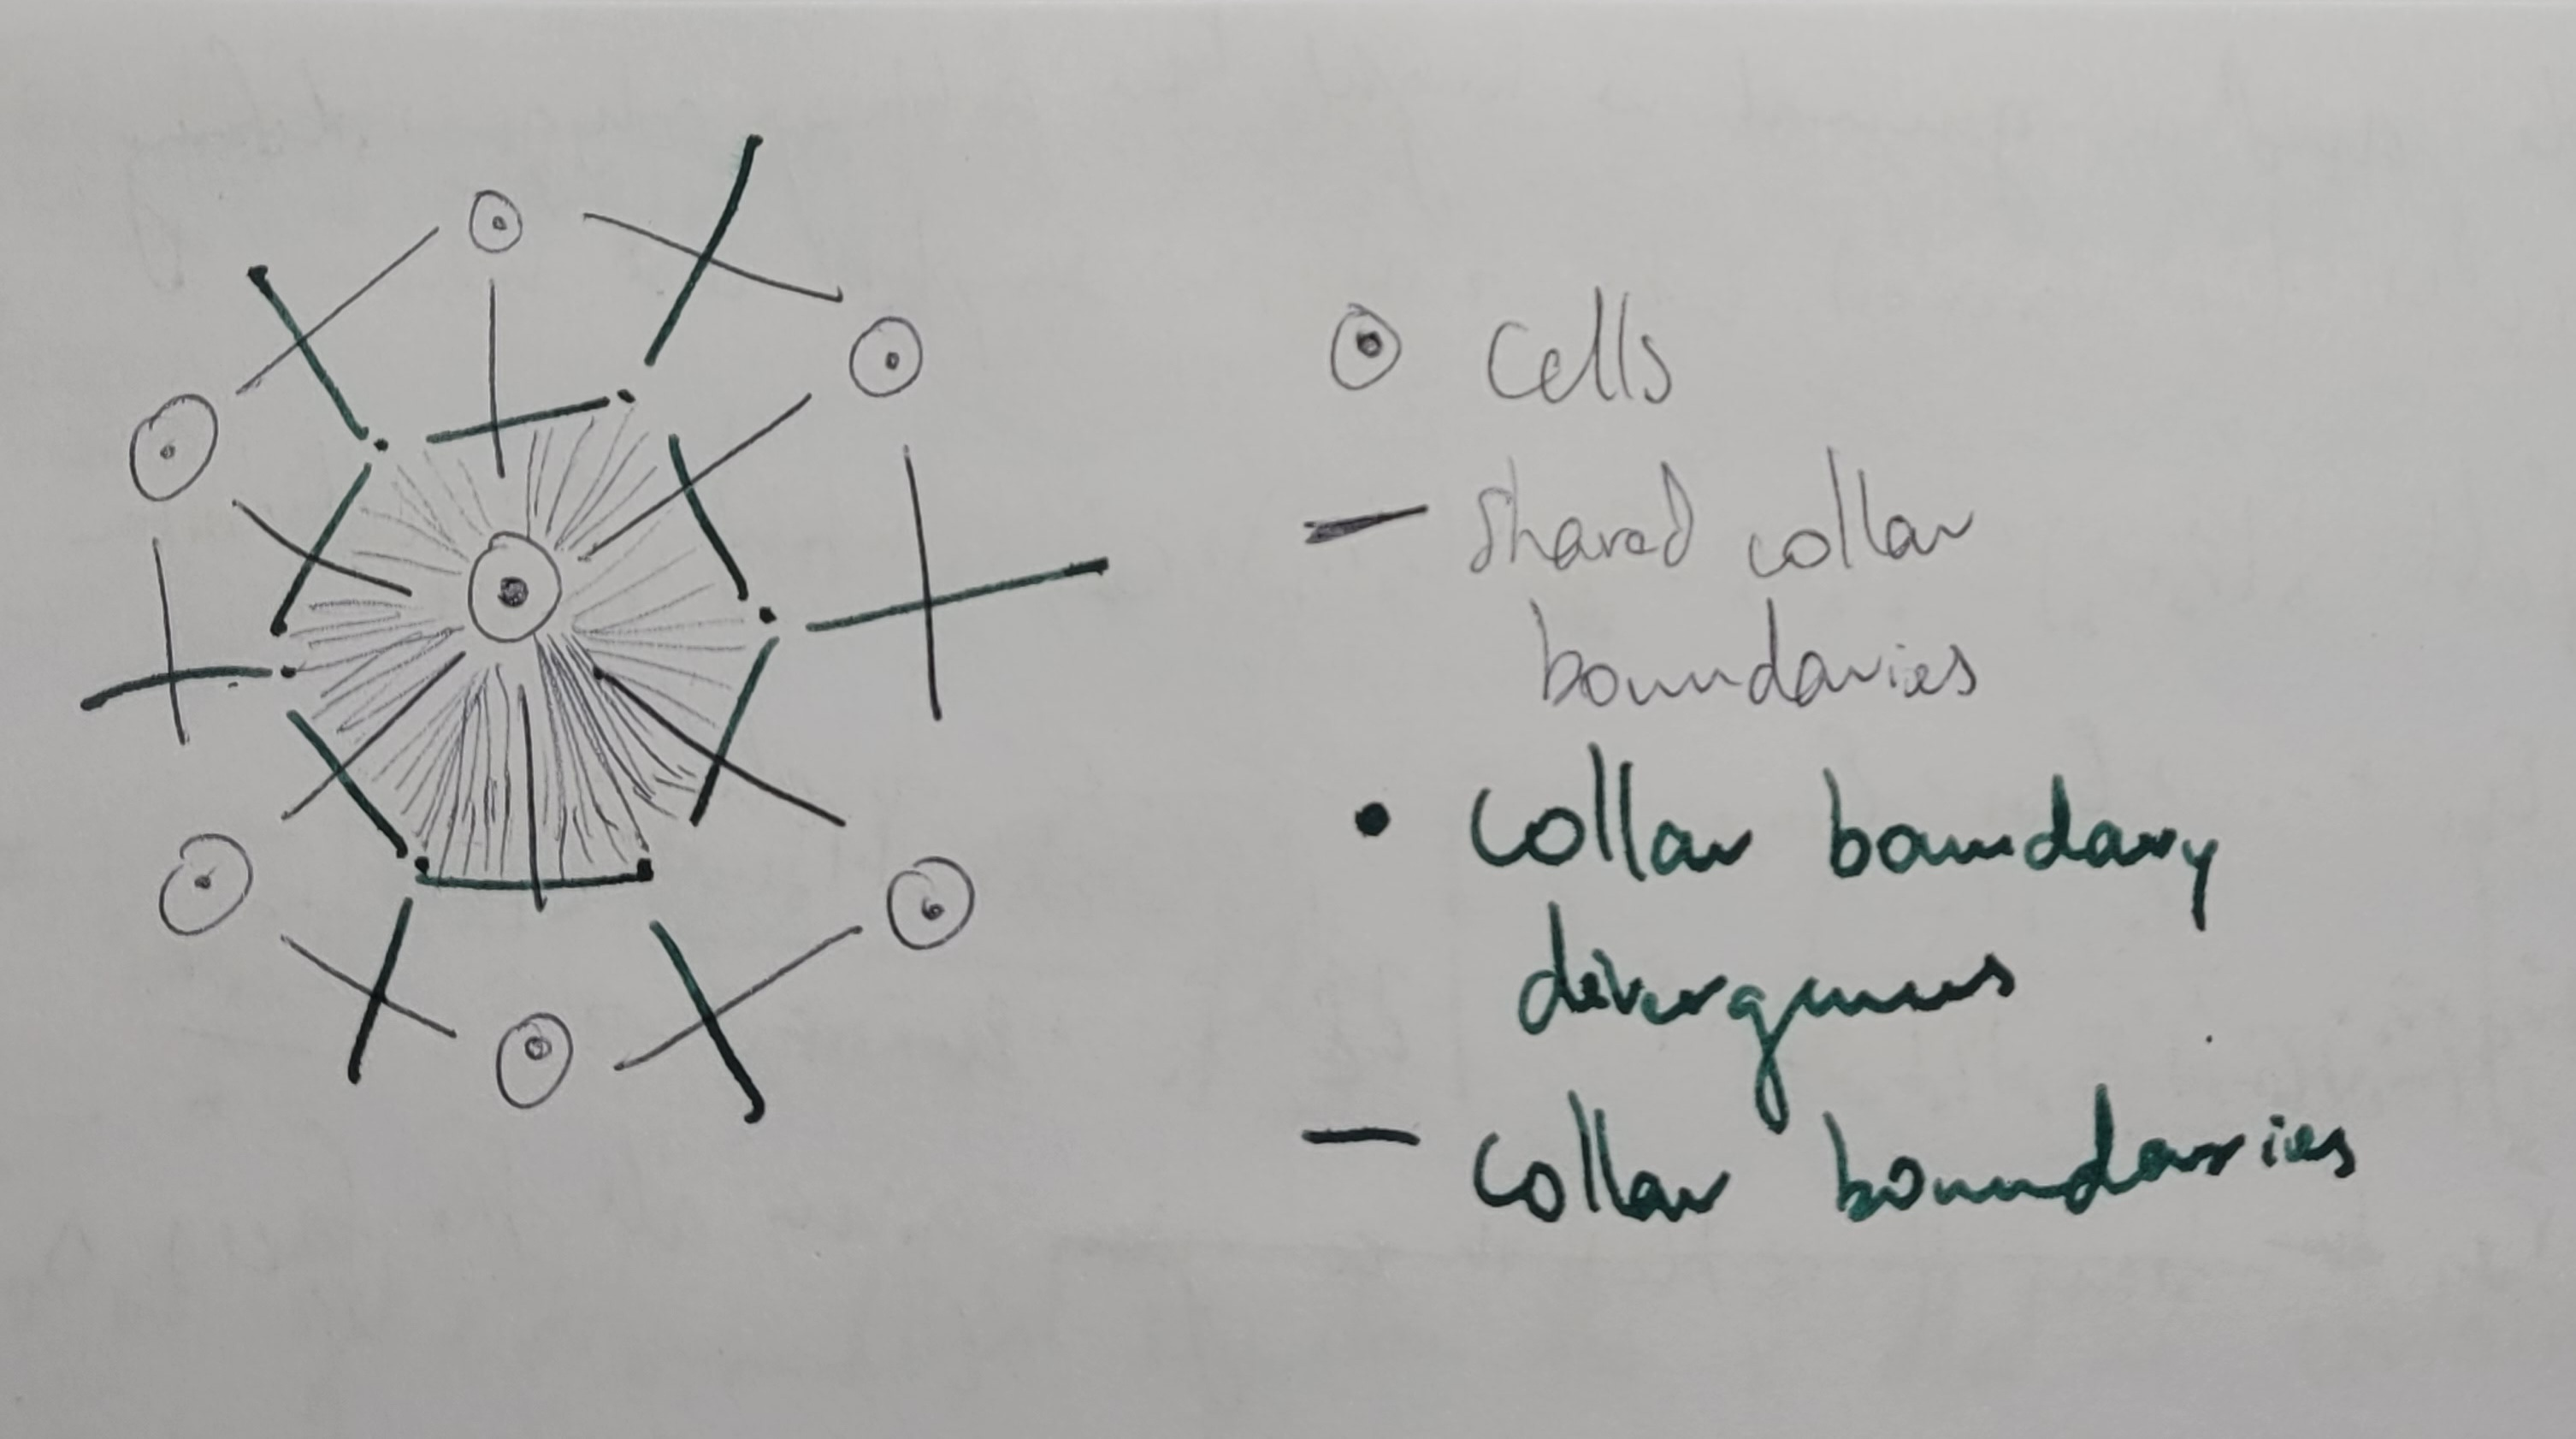
\includegraphics[width=\textwidth]{figures/duals1.jpg}
        \caption{}
        \label{subfig:duals1}
    \end{subfigure}
    ~
    \begin{subfigure}[b]{0.46\textwidth}
        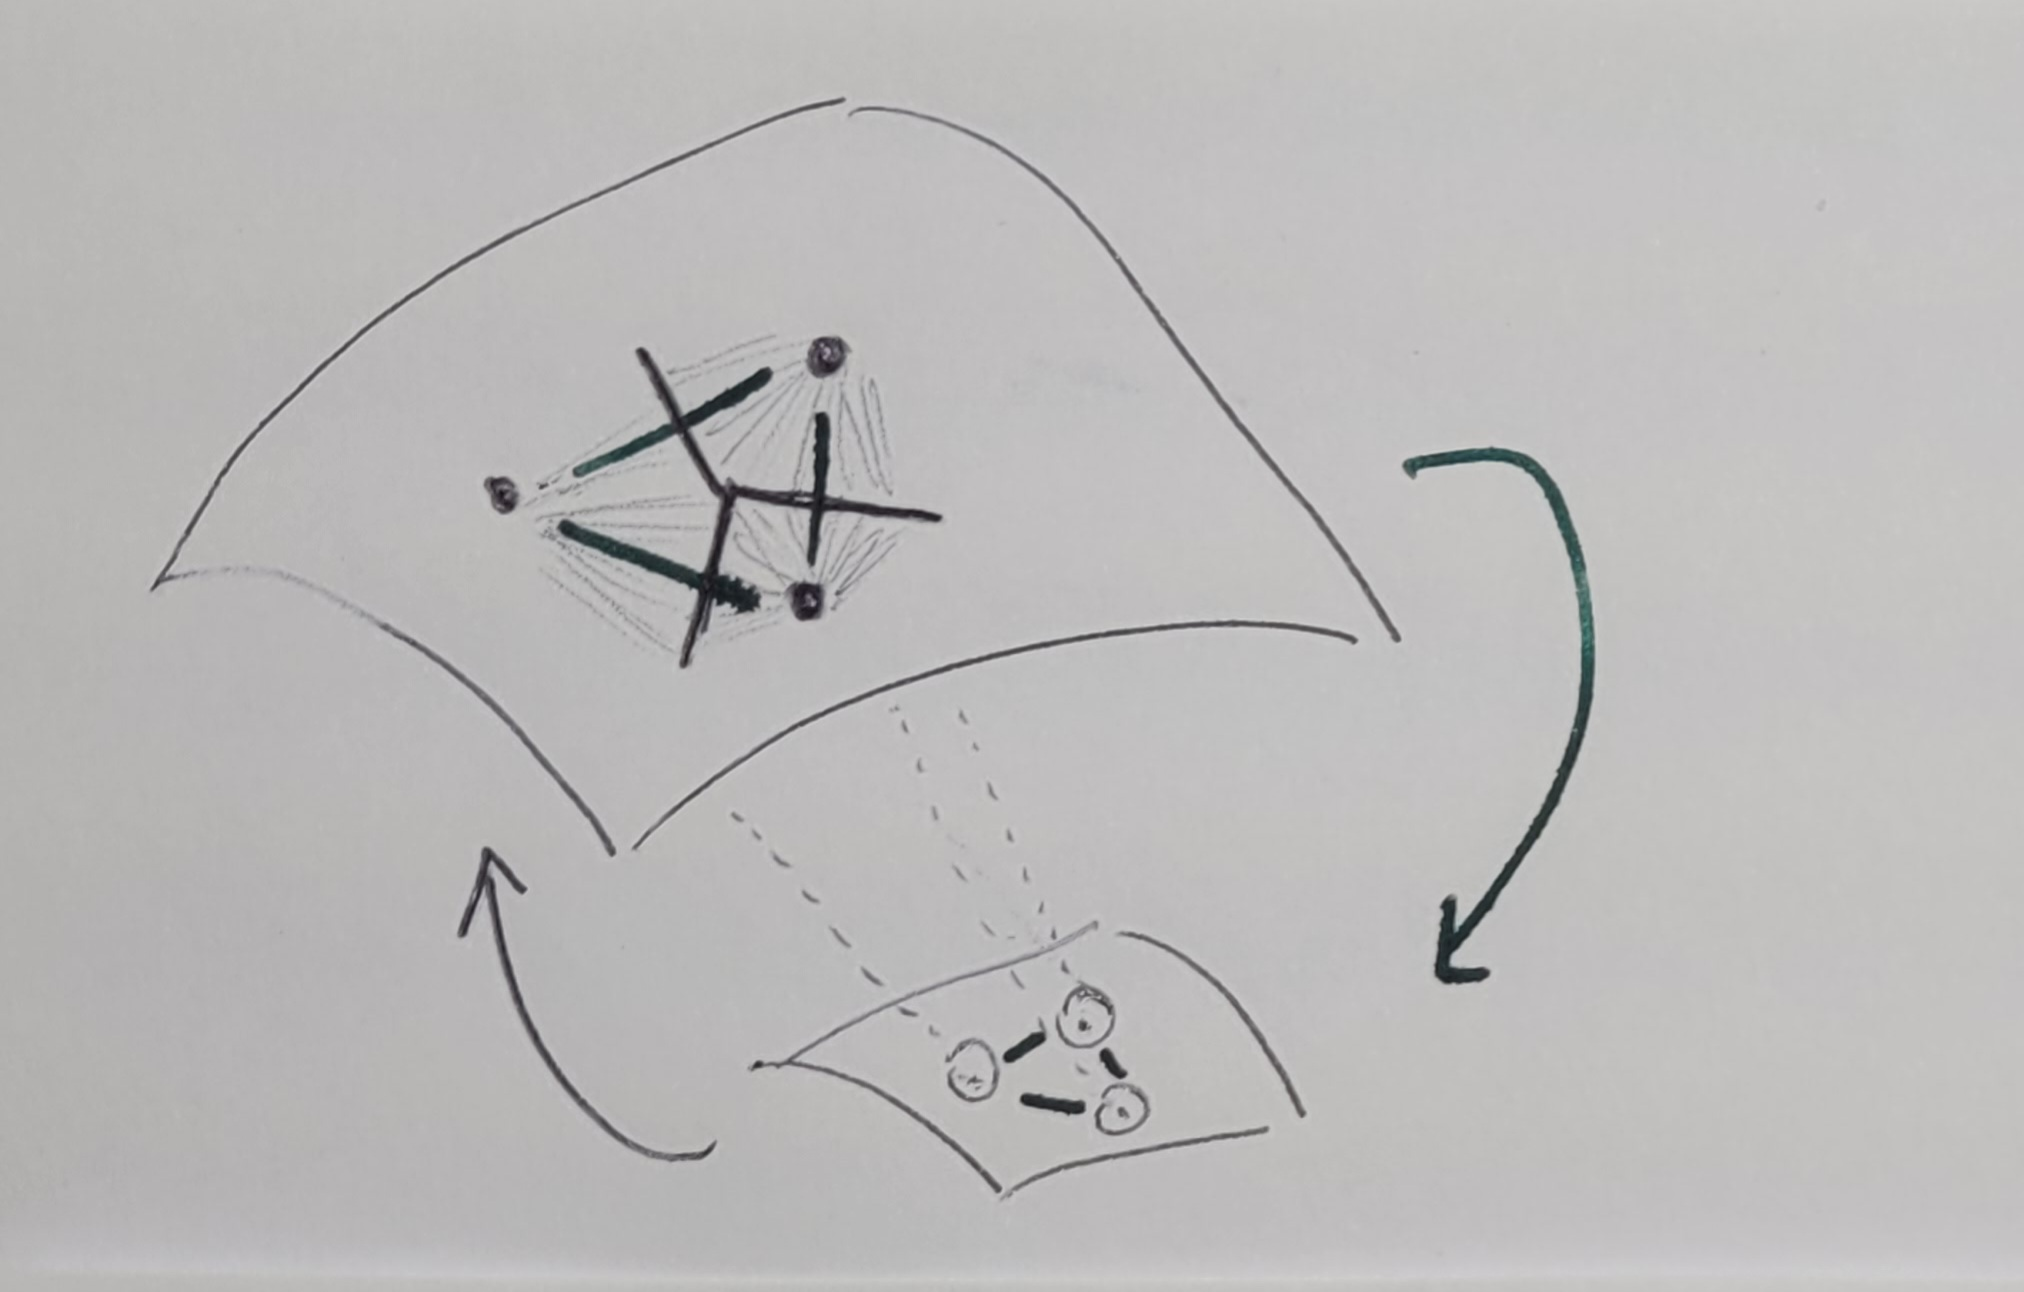
\includegraphics[width=\textwidth]{figures/duals2.jpg}
        \caption{}
        \label{subfig:duals2}
    \end{subfigure}
    \caption{Two views of the physical dual graphs used in describing \textit{C. flexa}.}
    \label{fig:duals}
\end{figure}

\subsection{Surface formed by collar boundaries}
\subsubsection{Stretching}

The physical interactions happen at the collar boundaries, so it makes sense to define energy based on the graph that quantifies them. If two cells have a collar boundary described by $\bm{r_a} t + (1-t)\bm{r_b}$ with $0 \leq t \leq 1$ and the energy is defined by continuously many springs from the boundary to a projected cell point $\bm{r_\Delta}$, then the energy $\e_{ab}$ of that boundary is 

\begin{align}
    \e_{ab} = \int_0^1 \left[(\bm{r_a}t + (1-t)\bm{r_b}) - \bm{r_\Delta} \right]^2 dt &= \frac{1}{3} (\bm{r_a} + \bm{r_b})^2 - \frac{1}{3} \bm{r_a}\cdot\bm{r_b} - \bm{r_\Delta} \cdot (\bm{r_a} + \bm{r_b}) + \bm{r_\Delta}^2. \label{eq:eab}
\end{align}

The energy corresponding to a cell consists of the line energies of all the collar interfaces. We find the position $\bm{r_\Delta}$ by setting the gradient of equation \ref{eq:eab} with respect to $\bm{r_\Delta}$ to zero for all lines $ab$. If $b$ indexes the vertices that cell $\Delta$ has, then 

\begin{align*}
    0 = \frac{d\e}{d\bm{r_\Delta}} &= -\sum_{b\in\Delta} \bm{r_b} + 2n\bm{r_\Delta} \\
    \bm{r_\Delta} &= \frac{1}{n} \sum_{b\in\Delta} \bm{r_b}.
\end{align*}

The force on vertex $a$ is then given by the gradient of the whole sheet energy $\e_{\text{sheet}}$, which is the sum of the energies $\e_\Delta$ corresponding to each cell $\Delta$. 

\begin{align*}
    \frac{d \e_{\text{sheet}}}{d\bm{r_a}} &= \frac{d}{d\bm{r_a}} \sum_\Delta \e_\Delta = \sum_{\Delta:a \in \Delta} \frac{d\e_\Delta}{d\bm{r_a}} = \sum_{\Delta:a\in\Delta} \frac{d}{d\bm{r_a}} \sum_{b \in \Delta} (\bm{r_b} - \bm{r_\Delta})^2. \\
    \intertext{Since $\bm{r_\Delta}$ depends on $\bm{r_a}$ itself, we write} \\
    \bm{f_{\text{on }a}} &= -\sum_{\Delta:a\in\Delta} \frac{d}{d\bm{r_a}} \sum_{b \in \Delta} \left(\bm{r_b} - \frac{1}{n} \sum_{c\in\Delta} \bm{r_c} \right)^2 \\
    &= \sum_{\Delta:a\in\Delta} \sum_{b \in \Delta} \left(2\bm{r_a}\delta_{ab} - \frac{2}{n} \sum_{c\in\Delta}\left(\bm{r_c}\delta_{ab} + \bm{r_b}\delta_{ac}\right) + \frac{1}{n^2} \sum_{c\in\Delta}\sum_{d\in\Delta} \left(\delta_{ac}\bm{r_d} + \delta_{ad}\bm{r_c} \right) \right) \\
    &= -2\left(\bm{r_a} - \bm{r_\Delta} \right)
\end{align*}

This process was overkill, since we could have reasonably assumed that $\bm{r_\Delta}$ would be at the vertices' center of mass and that we'd effectively get springs from $\bm{r_\Delta}$ to each vertex. This is thanks to linearity of the collar springs. However, assuming that the collars have a positive equilibrium length $r_0$ makes it necessary to go through the above procedure.

If instead the line energy is 

\begin{align*}
    \e_{ab} &= \int_0^1 \left(\left|\bm{r_a}t + (1-t)\bm{r_b} - \bm{r_\Delta}\right| - r_0 \right)^2 dt, \\
    \intertext{then the cell position $\bm{r_\Delta}$ is the solution to} \\
    0 &= -2 \sum_{b\in\Delta} \bm{r_b} + 6 \bm{r_\Delta} - 2r_0 \frac{d}{d\bm{r_\Delta}} \sum_{(b,c) \text{ edge in }\Delta} \int_0^1 \left| \bm{r_b}t - (1-t)\bm{r_c} - \bm{r_\Delta} \right| dt \\
    0 &= -2 \sum_{b\in\Delta} \bm{r_b} + 6 \bm{r_\Delta} - 2r_0 \sum_{(b,c)} \int_0^1 \frac{\bm{r_\Delta} - \bm{r_c} - t(\bm{r_b} - \bm{r_c})}{\left|\bm{r_b}t - (1-t)\bm{r_c} - \bm{r_\Delta} \right|} dt.
\end{align*}

We can actually evaluate the integral above, but I found that it gives a transcendental equation for $\bm{r_\Delta}$ and decided it wasn't pursuing further on paper. Nonzero equilibrium length springs is better pursued numerically. Alternatively, we simply define springs from $\bm{r_\Delta}$ to each dual graph vertex rather than making the collars consist of continuous springs.

\subsubsection{Bending}

One way to define a bending energy is to give each cell a vector that corresponds to the midline pointing out from the center of the cell, which I have implicitly drawn in the figures of individuals flexas. From there, we could reasonably define a bending energy from the interactions between two interacting flexas by the angle between their corresponding ``normal'' vectors weighted by the length of their interface. 

Defining an individual vector is made complicated by the fact that the vertices along the cycles corresponding to each flexa are not necessarily coplanar, provided that a given cell is interacting with more than three other cells. One option, although I have not developed it, is to find the plane whose summed mean squared distances to each vertex for a cell is minimised. It would possibly be more accurate to again treat the edges as lines and minimise the integrated distance from the normal plane to the edges. Either way, the energy dictated by the angle between adjacent normal vectors will need to be summed over all pairs of neighboring cells, namely all edges in the graph where edges correspond to cell neighbors (not collar interfaces).

\subsection{Surface formed by cell bodies}

The graph of cell bodies and neighbor edges makes it easy to work with springs, but it is less clear how to define a bending energy. The math for springs is identical to previously, so let's just think about how to define bending energy.

\textbf{needs more work}

% \subsubsection{Bending}

\section{Including both cells and collar boundaries}

\subsection{Initial sheet}
Let's call the graph of cells with cell-cell neighbor relations as edges $G$, and the dual graph of collar boundaries $G^*$. For setting up the network topology, we proceed by defining $G$ to lie in the $xy$-plane with a set of cell coordinates $\{\bm{r}_c\}_{c\in C}$ for the set of cells $C$ and using Voronoi tessellation to build $G^*$. This is nice because it generalises beyond regular lattices. The curvature will be built in later when minimising the sheet energy.

We can build a super graph $\mathfrak{G}$ which has both the cell positions and collar boundaries, as well as edges from each cell $c$ to the boundary vertices $b$ in the cell's set of collar boundary vertices $B_c \in V^*$. That is, $\mathfrak{G}$ has the cell-cell neighbor edges $E$ between cell vertices $C$, collar vertices $V^*$, and edges $\{ \{(c, b)\}_{b\in B_c} \}_{c\in C}$. 

Since Voronoi regions for cells that aren't completely surrounded by other cells (which I will call \textit{boundary cells}) extend out to infinity, we need to create a new vertex at each infinite boundary to make a finite collar boundary. (Figure \ref{fig:voronoi})

\begin{figure}[htbp]
    \centering
    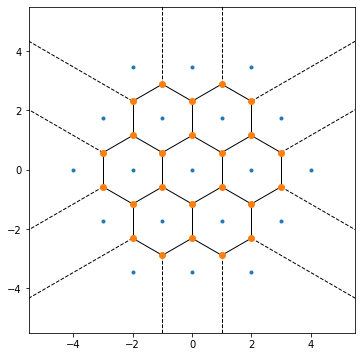
\includegraphics[width=0.5\textwidth]{figures/numerical/voronoi.png}
    \caption{Voronoi tesselation of initial cell placement. Cell bodies shown in blue points, collar boundaries shown in black lines with collar boundary end points shown in orange. Notably, the regions corresponding to boundary cells extend out to infinity. We need to add all boundary collar vertices along the infinite dashed lines.}
    \label{fig:voronoi}
\end{figure}

\subsubsection{Why do boundary collar vertices matter?}

Does it matter that boundary cells have collar nodes at the boundary? We can answer this analytically. For cells $a, c$ and mutual interior collar boundary vertex $b$, suppose the physically finite collar boundary ends at point $\bm{r}$. We want to know how the angle between the planes $\bm{r}_a, \bm{r}_b, \bm{r}$ and $\bm{r}_c, \bm{r}_b, \bm{r}$ changes as $\bm{r}$ changes. 

For now let's say that the collar length is fixed as $\ell$, so the range of motion of $\bm{r}$ is constrained. We can simplify our problem by reparameterising our coordinates such that $\bm{r}_a = (-1, 0, 0)$, $\bm{r}_b = (0, r, 0)$, and $\bm{r}_c = (1, 0, 0)$, where $r = \sqrt{\ell^2 - 1}$. Note that $\ell$ is a dimensionless ratio of the collar length to cell-cell distance here.\footnote{Later we will use $\ell$ as the only length scale in the problem when we're solving the sheet shape by minimising energy.} It is easy to show that the solution set for allowable values of $\bm{r}$ is given by solutions satisfying $r^2 = y^2 + z^2$, $x=0$. Equivalently, the possible vectors $\bm{r}(\theta)$ are $(0, r\cos\theta, r\sin\theta)$. So let's find the normal vectors between the two collar-cell-collar surfaces to see if the plane-plane angle changes with $\theta$. 

We have the normals are 
\begin{align*}
    \hat{\bm{n}}_1 &= (\bm{r} - \bm{r}_a) \times (\bm{r}_b - \bm{r}_a) \\
    &= \frac{(-r^2 \sin\theta, r\sin\theta, r - r\cos\theta)}{r^4\sin^2\theta + 2r^2(1-\cos\theta)} \\
    \hat{\bm{n}}_2 &= (\bm{r}_b - \bm{r}_c) \times (\bm{r} - \bm{r}_c)\\
    &= \frac{(r^2 \sin\theta, r\sin\theta, r\cos\theta - r)}{r^4\sin^2\theta + 2r^2(1-\cos\theta)}.
\end{align*}
\noindent Their angle is given by (after simplifying)
\begin{align*}
    \hat{\bm{n}}_1 \cdot \hat{\bm{n}}_2 &= 1 - \frac{2}{1 + \frac{1}{2r^2} \left(1+\tan^2\frac{\theta}{2}\right)}.
\end{align*}

The point is that the plane-plane angle changes with $\theta$! So the boundary collar nodes really have an effect on the sheet energy, and we need to include them. This is an important result too since (as Lloyd always reminds me) the boundary conditions affect the whole shape of the sheet. So one way to conceivably move the sheet is by updating the boundary collar nodes then working inward to update the whole sheet shape. 

Regardless, this tells us that we need to add our own boundary collar nodes to our simulation, since they aren't provided by the Voronoi tessellation.

\subsubsection{Adding boundary collar vertices}

The coordinate system for each cell-cell neighbor pair we developed in the previous section is useful for creating our own new boundary collar vertices. For two boundary cell positions $\bm{r}_{c_1}, \bm{r}_{c_2}$, we can take the orthogonal component of $\bm{r}_{b} - \bm{r}_{c_1}$ (where $b$ is the existing collar boundary node between $c_1, c_2$) with respect to $\bm{r}_{c_1} - \bm{r}_{c_2}$. Adding this orthogonal component to the cells' center of mass $(\bm{r}_{c_1} + \bm{r}_{c_2})/2$ (which is on the Voronoi boundary) will give a new position equidistant from the two cells, where the cell-collar lengths is the same as that to the existing collar boundary vertex. 

\begin{figure}[hbtp]
    \centering
    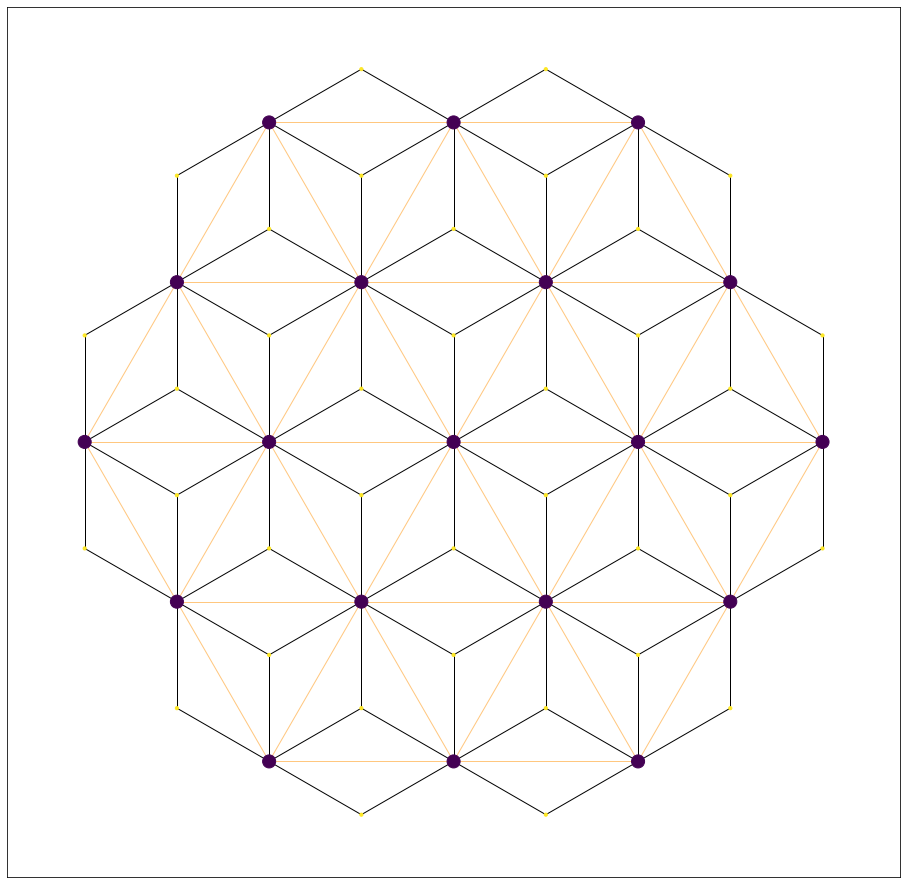
\includegraphics[width=0.8\textwidth]{figures/numerical/layout_init.png}
    \caption{Initial layout for the flexa sheet. Cell bodies are shown in large purple points and collar boundary vertices are shown in small yellow points. Black edges connect cells to collar boundary vertices, and orange edges show cell-cell neighbor relations (though these orange edges are not physically present). The physical interactions are mediated through the black edges.}
    \label{fig:layout_init}
\end{figure}

The resulting cell sheet and collar boundary surface is shown in Figure \ref{fig:layout_init}. Notice in particular that every cell on the boundary has two collar nodes between it and its neighboring cells on the boundary. This whole graph $\mathfrak{G}$ is shown projected onto the $xy$-plane, but the collar interactions are all offset in $z$ relative to the cells. 

\subsection{Bending energies}

\subsubsection{Collar length}
For now, we are going to take the collar lengths to be fixed at their initial lengths. Since we're using a regular lattice for now, we can define this as $\ell$ to be the only length in our problem. (Cell-cell distance will change when we minimise the energy.)

Later, it would be nice to add a collar length energy term $(|\bm{r}_c - \bm{r}_{b_{c}}| - r_0)^2$ term that makes the cell-collar lengths flexible.

\subsubsection{Cell-collar angle $\phi$ energy}

The paper we're basing our work on defines the collar angle $\phi$ relative to the direction of the cell body $\hat{n}_c$ for cell $c$. Immediately, we run into a problem, which is that $\hat{n}$ is not clearly defined when the cell is interacting with several other cells. When that happens, the cell's collar does not necessarily form its boundaries in a plane. 

\paragraph{Defining the cell normal vector $\hat{n}_c$}
We can define the cell's vector $\hat{n}_c$ for a cell $c$ by taking the average vector from $\bm{r}_c$ to $\bm{r}_b$ for all collar boundary nodes $b \in B_c$. However, we run into a problem for boundary cells, which is that this normal vector then points inward towards the sheet because we didn't define collar boundary nodes that don't connect to other cells. In the language of Figure \ref{fig:layout_init}, the boundary cells have less than a symmetric set of 6 collar boundary nodes. 

This doesn't agree with our intuition, since the entire sheet is flat. So we expect the cells at the boundaries to have vectors $\hat{n}_c$ pointing directly in $+\hat{\bm{z}}$ (as the collars are above the cell sheet in $z$). Instead, we can define $\hat{n}_c$ by taking a plane approximation to the collar boundary position vectors $\{ \bm{r}_b \}_{b \in B_c}$. This plane defines a normal vector.

If we approximate $\hat{z}_b = (x_b, y_b)\cdot (\beta_1, \beta_2) + \beta_0$ and minimize the sum of squared residuals $\sum_{b\in B_c} (\hat{z}_b - z_b)^2$ with respect to $\beta_0, \beta_1, \beta_2$,\footnote{We do this with ordinary least squares, which is why I use the notation $\hat{z}_b$ and $\bm{\beta}$.} then the normal vector of the plane approximation is $(\beta_1, \beta_2, -1)$ up to normalisation and multiplication by $-1$. 

We need to orient the cell's vector $\hat{\bm{n}}_c$ so that it points in the direction from the cell to the collar. Fortunately, we could use the average cell-to-collar vector that we discussed before to do this alignment. 

\paragraph{What is the best normal vector for a cell?}

Suppose a cell is at position $\bm{r}_c$ with collar vertices at $\bm{r}_b$ for $b \in B_c$. We can ask how the cell orients itself to minimise its collar energy in $\phi$. The energy of the cell $\e_c$ is given by 

\begin{align*}
    \e_c &= \sum_{b\in B_c} \left[ \arccos\left(\frac{\bm{r}_b - \bm{r}_c}{\left|\bm{r}_b - \bm{r}_c\right|} \cdot \hat{n}_c \right) - \phi_0 \right]^2. \\
    \intertext{We can ask what normal vector minimises $\e_c$ by setting the gradient of $\e_c$ with respect to $\hat{\bm{n}}_c$ to zero. But the length of $\hat{\bm{n}}_c$ is fixed at one, so we solve } \\
    0 &= \frac{\partial \left[ \e_c + \lambda\left( \left| \hat{\bm{n}}_c\right|^2 - 1\right) \right] }{\partial \hat{\bm{n}}_c} \\
    \intertext{subject to $\left| \hat{\bm{n}}_c\right|^2 = 1$. I found that } \\
    \lambda \hat{\bm{n}}_c &= 2 \sum_{b \in B_c} \left[ \arccos\left(\frac{\bm{r}_b - \bm{r}_c}{\left|\bm{r}_b - \bm{r}_c\right|} \cdot \hat{n}_c \right) - \phi_0 \right] \frac{-1}{\sqrt{1 - \left(\frac{\bm{r}_b - \bm{r}_c}{\left|\bm{r}_b - \bm{r}_c\right|} \cdot \hat{n}_c \right)^2 }}\frac{\bm{r}_b - \bm{r}_c}{\left|\bm{r}_b - \bm{r}_c\right|}
    \\
    \lambda &= 2 \left| \sum_{b\in B_c} \left[\arccos\left(\frac{\bm{r}_b - \bm{r}_c}{\left|\bm{r}_b - \bm{r}_c\right|} \cdot \hat{n}_c \right) - \phi_0 \right]
    \frac{1}{\sqrt{1 - \left(\frac{\bm{r}_b - \bm{r}_c}{\left|\bm{r}_b - \bm{r}_c\right|} \cdot \hat{n}_c \right)^2 }}
    \frac{\bm{r}_b - \bm{r}_c}{\left|\bm{r}_b - \bm{r}_c\right|} \right|. \\
    \intertext{Then } \\
    \hat{\bm{n}}_c &= \frac{\sum_{b \in B_c} \left[ \arccos\left(\frac{\bm{r}_b - \bm{r}_c}{\left|\bm{r}_b - \bm{r}_c\right|} \cdot \hat{n}_c \right) - \phi_0 \right] \frac{-1}{\sqrt{1 - \left(\frac{\bm{r}_b - \bm{r}_c}{\left|\bm{r}_b - \bm{r}_c\right|} \cdot \hat{n}_c \right)^2 }}\frac{\bm{r}_b - \bm{r}_c}{\left|\bm{r}_b - \bm{r}_c\right|}}{\left| \sum_{b'\in B_c} \left[\arccos\left(\frac{\bm{r}_{b'} - \bm{r}_c}{\left|\bm{r}_{b'} - \bm{r}_c\right|} \cdot \hat{n}_c \right) - \phi_0 \right]
    \frac{1}{\sqrt{1 - \left(\frac{\bm{r}_{b'} - \bm{r}_c}{\left|\bm{r}_{b'} - \bm{r}_c\right|} \cdot \hat{n}_c \right)^2 }}
    \frac{\bm{r}_{b'} - \bm{r}_c}{\left|\bm{r}_{b'} - \bm{r}_c\right|} \right|}
\end{align*}



\paragraph{Calculating collar angle $\phi$}
Once we have a cell normal vector $\hat{n}_c$ for each cell $c$, it is easy to calculate the collar angles $\phi_{cb}$ to each collar boundary vertex $b\in B_c$. Now, indexing over all cell-collar edges in $\mathfrak{G}$ (black edges in Figure \ref{fig:layout_init}), we write the $\phi$ energy
\begin{align*}
    \e_\phi &= \sum_{c\in C} \sum_{b \in B_c} (\phi_{cb} - \phi_0)^2 = \sum_{(c,b) \in \{\text{cell-collar edges }(c,b) \}} (\phi_{cb} - \phi_0)^2.
\end{align*}

When $\phi_0$ is equal to the initial angle between $\hat{\bm{z}}$ (which is the initial $\hat{n}_c$ for each cell $c$) and each cell-collar vector $\bm{r}_b - \bm{r}_c$ (which is well-defined because we're using a regular lattice to start), we get that $\e_\phi=0$ numerically. This confirms that our code is calculating the energy right. Of course this energy will be nonzero when $\phi_0$ differs from the initial angle. 

\subsubsection{Cell-cell junction angle $\psi$ energy}

We suppose that there is also an energy $\e_\psi$ based on the angle $\psi$ that two cells make at their mutual collar boundary. We can calculate this as we did previously, where we found that the length of collar boundary (equivalently, the angle $\theta$ between the two collar nodes and each cell) affects the cell-collar-cell angle. Let's say there's an equilibrium angle $\psi_0$ between two cell collars.

For cells $c_1, c_2$ and mutual collar boundary vertices $b, b'$, we define $\hat{\bm{n}}_1$ and $\hat{\bm{n}}_2$ as the normal vectors to planes defined by $\bm{r}_{c_1}, \bm{r}_b, \bm{r}_{b'}$ and $\bm{r}_{c_2}, \bm{r}_b, \bm{r}_{b'}$. The angle between these planes is given as $\hat{\bm{n}}_1 \cdot \hat{\bm{n}}_2$, and the acute angle on the interior of the hinge is $\pi - \arccos \left( \hat{\bm{n}}_1 \cdot \hat{\bm{n}}_2 \right)$. 

Let's assume that the angle $\psi$ is shared evenly between the two cells, so that the cell $c_1$ contribution to $\e_\psi$ is $(\psi_{c_1, c_2} / 2 - \psi_0/2)^2$ for cell-cell neighbor relation $(c_1, c_2)$. Likewise for $c_2$. Then $\e_\psi$ indexes over the cell-cell neighbor relations in edge set $E$:

\begin{align*}
    \e_\psi &= \sum_{(c_1, c_2) \in E} (\psi_{c_1, c_2} / 2 - \psi_0/2)^2.
\end{align*}

\subsubsection{Flat sheet as a solution} \label{subsubsec:flat}

Notice that we have a pair $(\phi_0, \psi_0)$ that gives $\e = \e_\phi + \e_\psi = 0$. Since the $\phi$ and $\psi$ energies are nonnegative, the flat sheet is a stable minimum. 

\subsection{Minimising sheet energy}

We now have an energy $\e\{ \bm{r}_v \}_{v \in \mathfrak{G}} = \e_\phi + \e_\psi$ which is parameterised over the cell and collar boundary vertex positions. Notably, we treat the topology of the network as fixed, so the indices of the summations for $\e_\phi$ and $\e_\psi$ are unchanged even as we minimise energy.

\subsubsection{Constant collar length constraint}

For now, we are numerically constraining the cell-collar lengths at $\ell$, their initial lengths (which are constant for all cells). If we want to use the generalisability of our model to use an random initial cell distribution and generate the irregular boundaries with Voronoi tesselation, we will have to relax this condition and add a collar length spring energy to $\e$. The constant collar length constraint only applies to sheets generated by regular lattices when laid flat on a plane.

The constraint is defined by a vector function $f((c, b)) = |\bm{r}_c - \bm{r}_b| - \ell = 0$ for all cell-collar edges $(c, b)$. If $n_{\text{collars}}$ is the number of cell-collar edges in $\{\text{cell-collar edges }(c,b) \}$, then $f$ defines a $n_{\text{collars}}$-vector function. 

My optimisation routine requires that we calculate a Jacobian matrix for the vector constraint function. This gets ugly if we use $f$ as written above, but it is fortunately equivalent to set the constraint $f'((c, b)) = |\bm{r}_c - \bm{r}_b|^2 - \ell^2 = 0$. It is an interesting problem to take the gradient of $\bm{f'}$ with respect to all of the coordinates, but I won't include it here. It's implemented in my code.

\subsection{Numerical optimisation routine}

Finally, we numerically optimise. I changed $\phi_0$ to be defined relative to the initial value of $\phi$, and likewise for $\psi$. If we make $\phi_0$ smaller and $\psi_0$ larger, we expect the cell collars to contract and for cell-cell distances to lengthen. In other words, we expect the sheet to curve upward, so that the cells on the edges go in the direction that the collars are.

The numerical optimisation problem gives a clean sensible solution, which is shown projected onto the $xy$-plane in Figure \ref{fig:layout_curved}. We can tell that the sheet is curved just looking at this alone, which is a massive relief and confirmation of what we expect.

\begin{figure}[htbp]
    \centering
    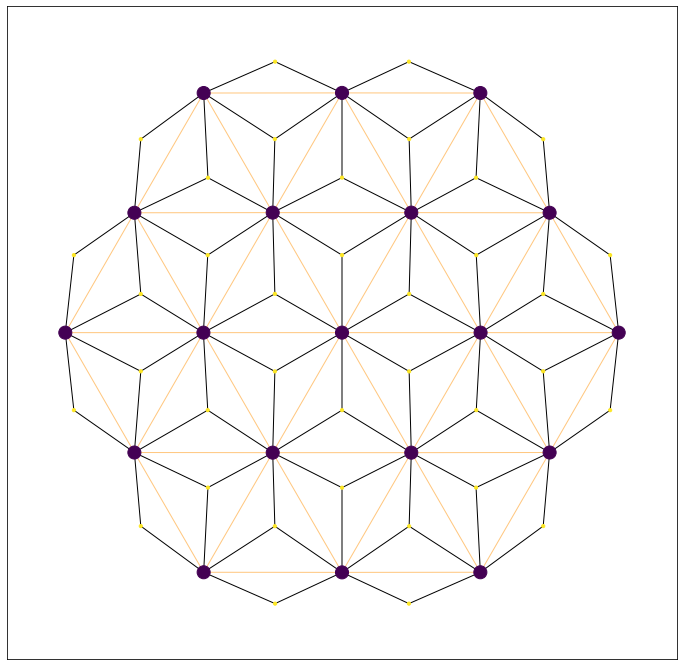
\includegraphics[width=0.8\textwidth]{figures/numerical/layout_curved.png}
    \caption{Figure in the same style of Figure \ref{fig:layout_init} showing the cell sheet projected onto the $xy$-plane after minimising energy. }
    \label{fig:layout_curved}
\end{figure}

The solution in Figure \ref{fig:layout_curved} is for $\phi_0 = 0.99 \phi_{\text{init}}$ and $\phi_0 = 1.03 \psi_{\text{init}}$, where $\phi_{\text{init}}$ and $\psi_{\text{init}}$ are the initial angles in the flat sheet state. We could now bask in the glory of our solution and look at it in 3d (Figure \ref{subfig:shallow}).

The resulting structure is really pretty sensitive to small changes in $\phi_0, \psi_0$. Figure \ref{subfig:deep} shows the structure that comes out of $\phi_0 = 0.9 \phi_{\text{init}}$, $\psi_0 = 1.15\psi_{\text{init}}$. 

\begin{figure}[htbp]
    \centering
    \begin{subfigure}[b]{\textwidth}
        \centering 
        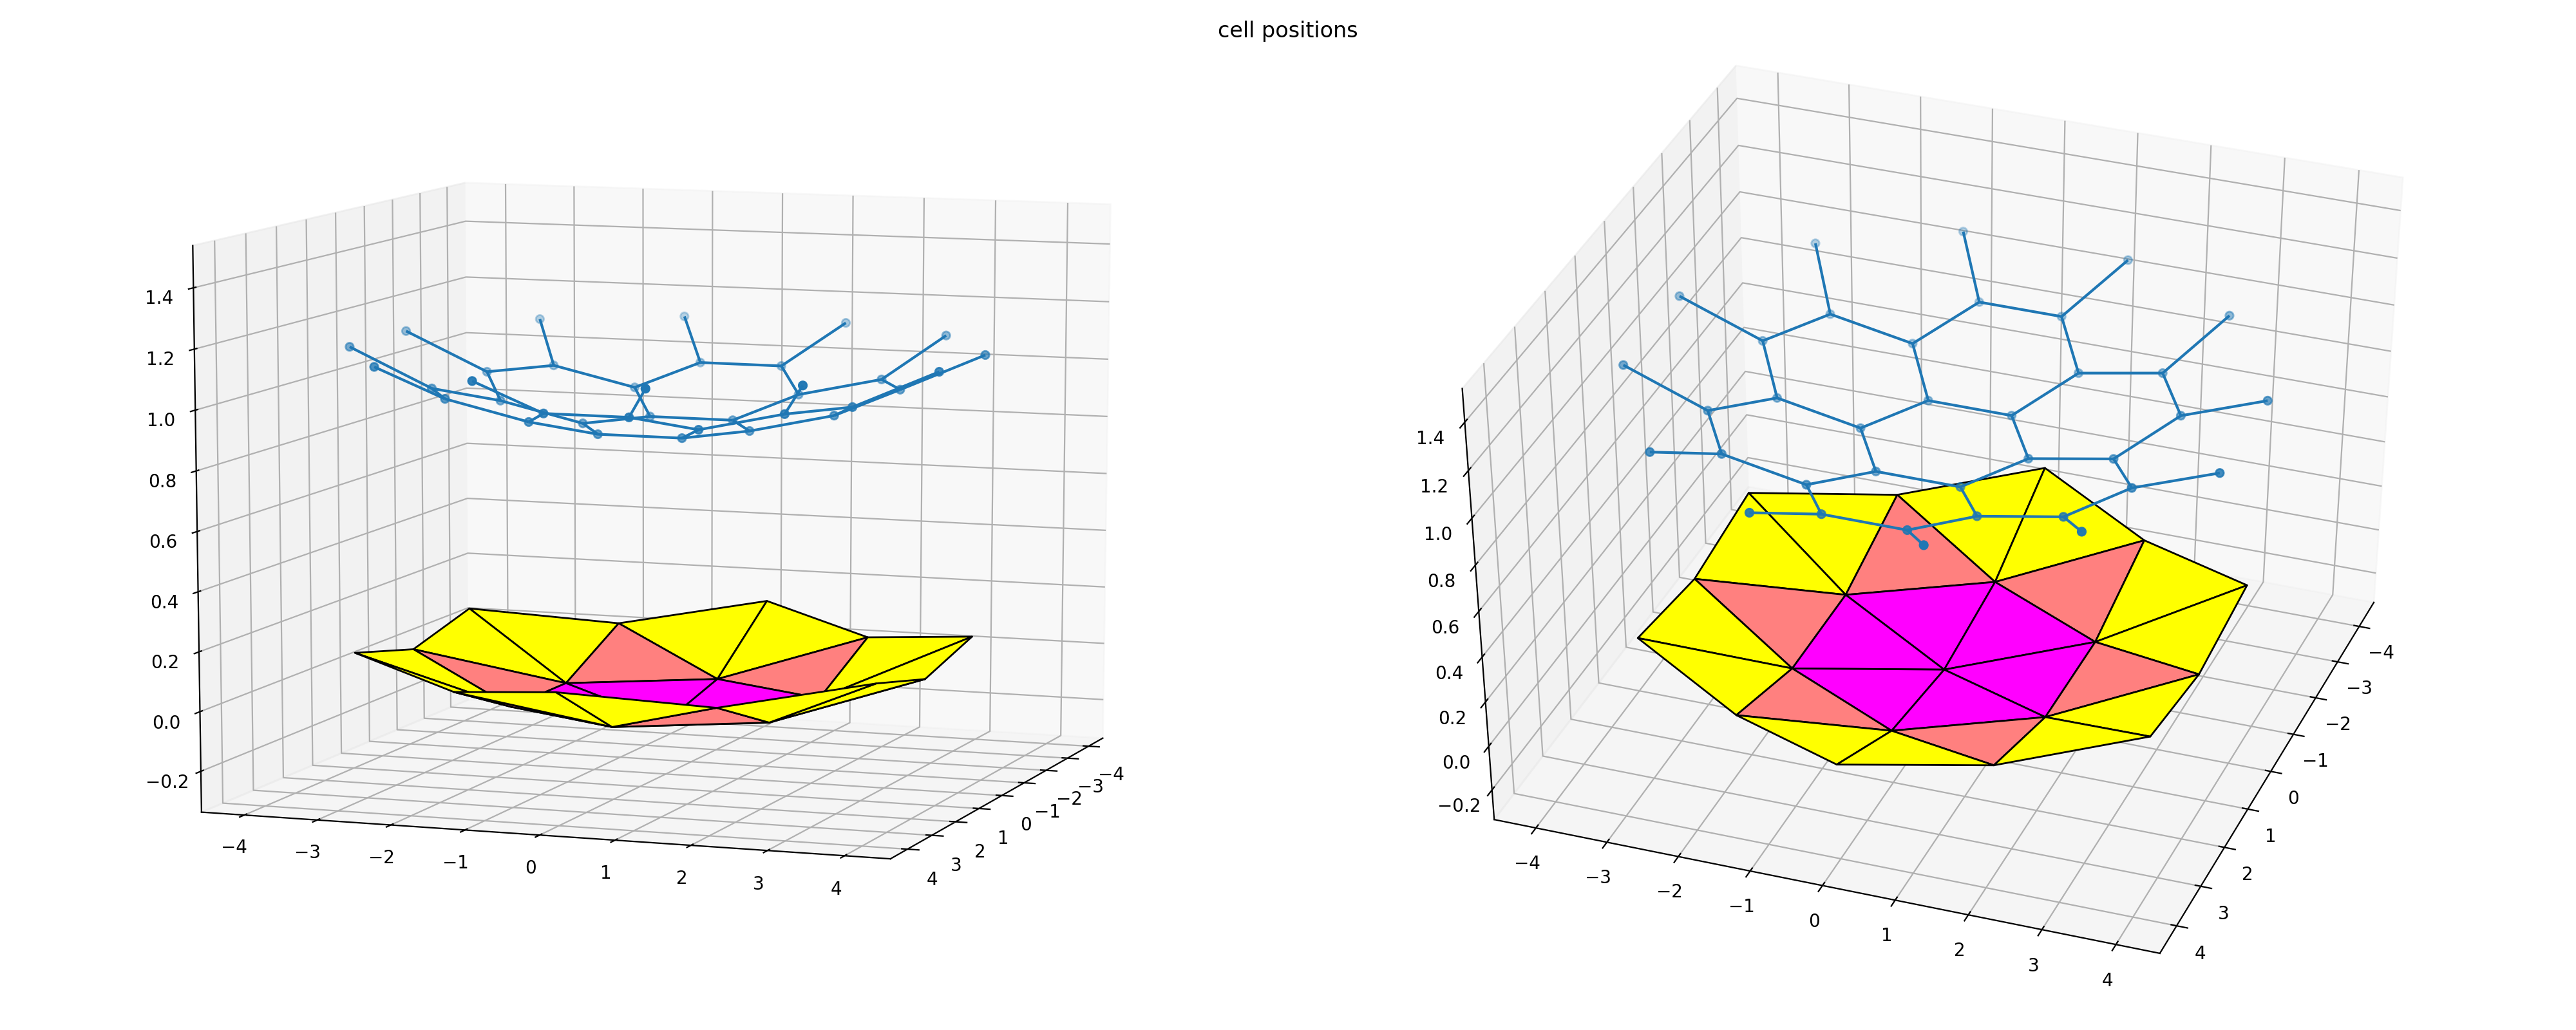
\includegraphics[width=\textwidth]{figures/numerical/shallow.png}
        \caption{}
        \label{subfig:shallow}
    \end{subfigure}
    \begin{subfigure}[b]{\textwidth}
        \centering
        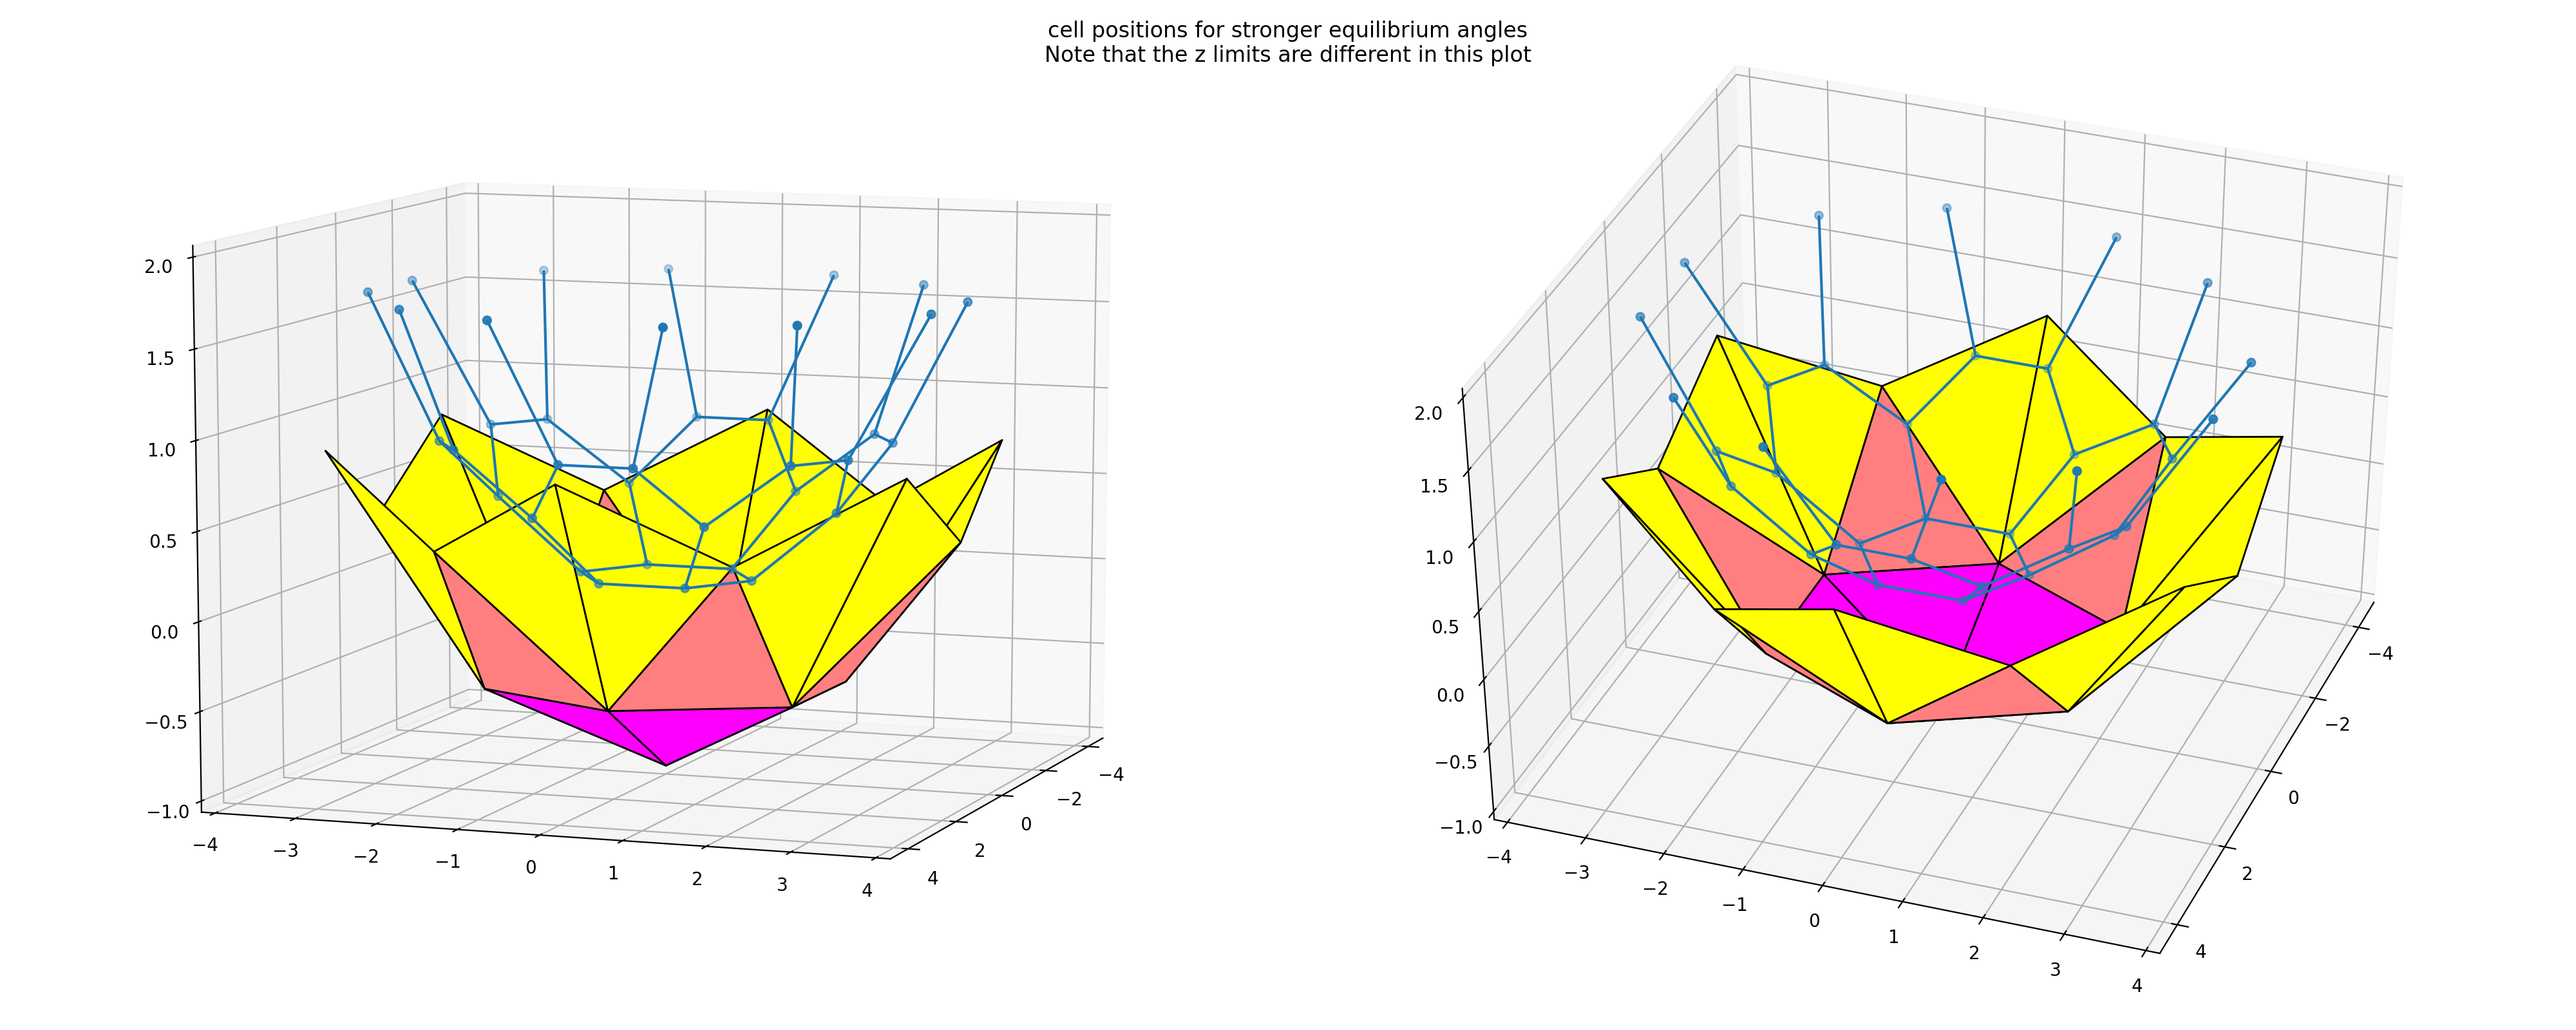
\includegraphics[width=\textwidth]{figures/numerical/deep.png}
        \caption{3d projections of the curved sheet formed by $\phi_0 = 0.9 \phi_{\text{init}}$, $\psi_0 = 1.15\psi_{\text{init}}$. }
        \label{subfig:deep}
    \end{subfigure}
    \caption{Cell sheet geometry from the hexagonal lattice in Figure \ref{fig:layout_init} and parameters (\ref{subfig:shallow}) $\phi_0 = 0.99 \phi_{\text{init}}$, $\phi_0 = 1.03 \psi_{\text{init}}$, $\ell_0 = \ell_{\text{init}}=1.52$, (\ref{subfig:deep}) $\phi_0 = 0.9 \phi_{\text{init}}$, $\psi_0 = 1.15\psi_{\text{init}}$, $\ell_0 = \ell_{\text{init}}=1.52$. }
\end{figure}

\subsection{Topology}

In section \ref{subsubsec:flat}, I mentioned that the flat sheet is a stable minimum. But it is here because the lattice is regular. A single pentagon in a hexagonal lattice (like a football (soccer) ball, thanks Lloyd) will make it so no $\phi_0$ and $\psi_0$ will make every cell make the other cells flat. 

What I think is interesting about this is the connection between graph topology and surface geometry. I think, in a continuous sense, graph topology affects Gaussian curvature through the energy function. 

\subsubsection{Adding noise to initial cell positions in Figure \ref{fig:layout_init}}

We expect the initial lattice in Figure \ref{fig:layout_init} to produce a sheet with 6-fold symmetry. Since the graph of connections is produced by a Voronoi tessellation, small changes to initial boundary cell positions can change the graph topology for boundary cells. 

When adding noise to the initial cell positions, the change in topology at some boundary nodes results in substantial effects felt over the sheet. Figure \ref{fig:hexnoise} shows the effect of different topology at the boundary.

\begin{figure}[htbp]
    \centering
    \begin{subfigure}[b]{\textwidth}
        \centering
        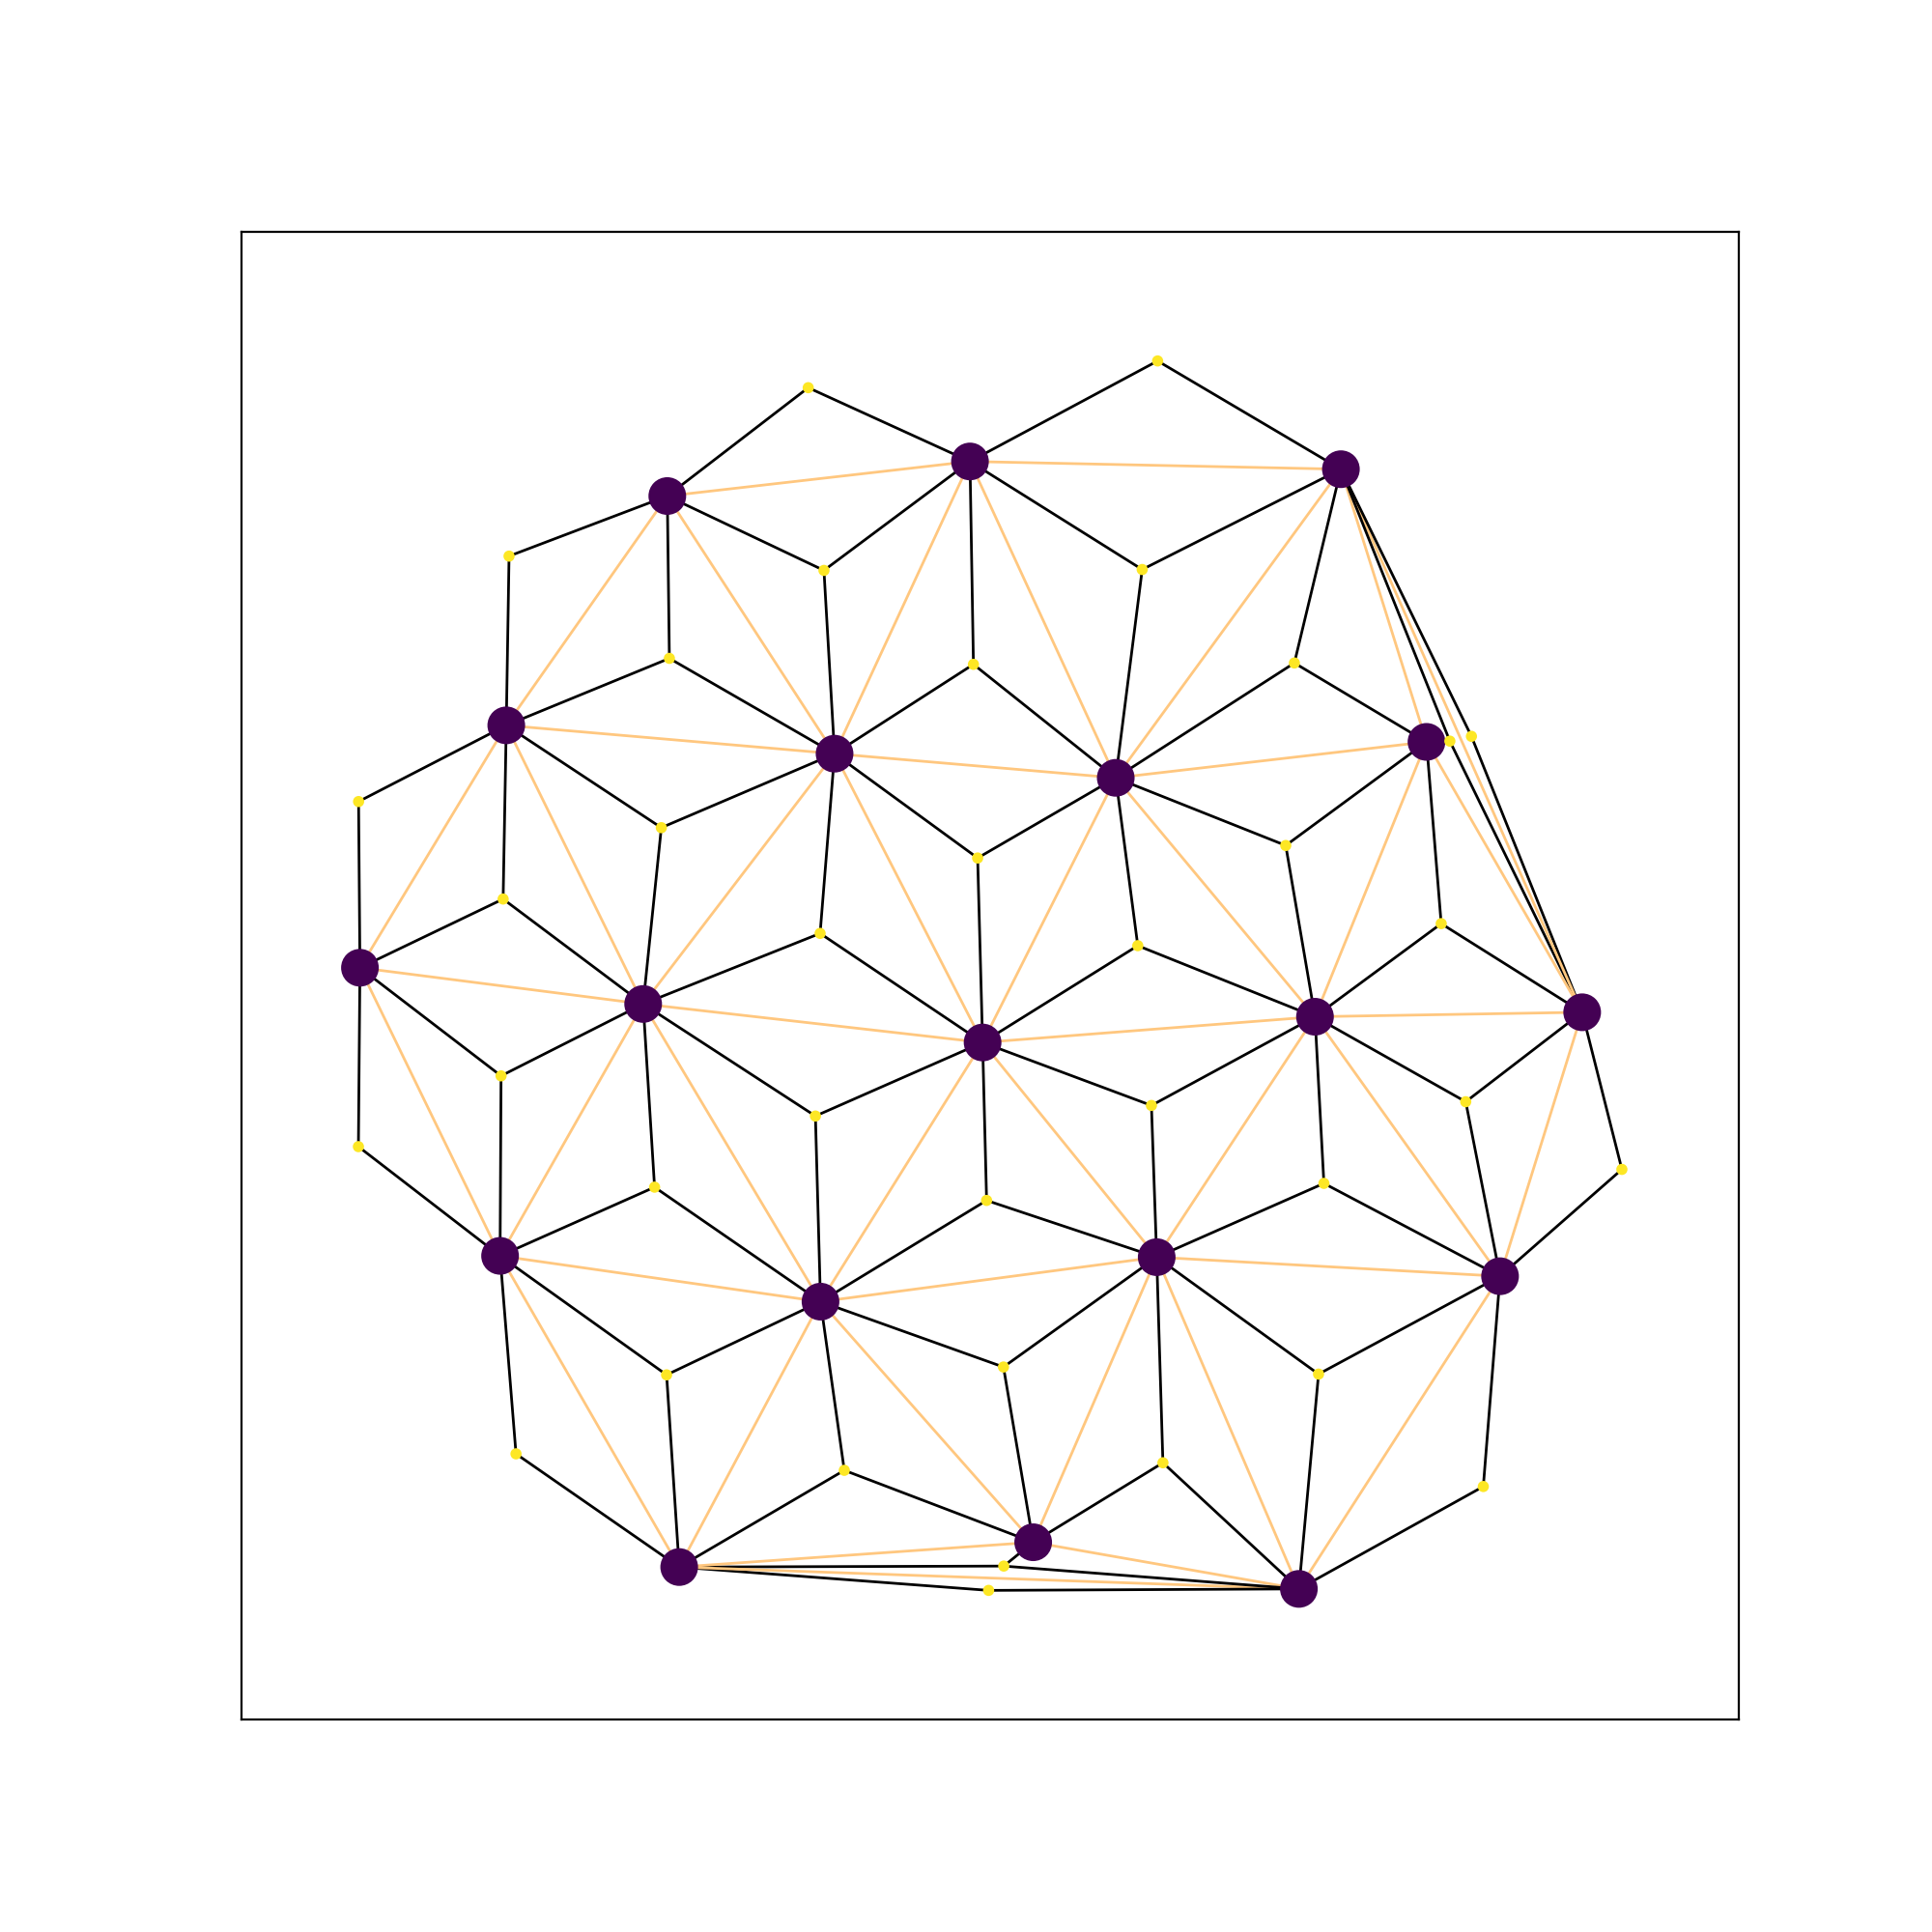
\includegraphics[width=0.5\textwidth]{figures/numerical/hexnoise/hexnoise_graph.png}
        \caption{Initial lattice drawn as in Figure \ref{fig:layout_init}.}
        \label{subfig:hexnoise_graph}
    \end{subfigure}
    \begin{subfigure}[b]{\textwidth}
        \centering
        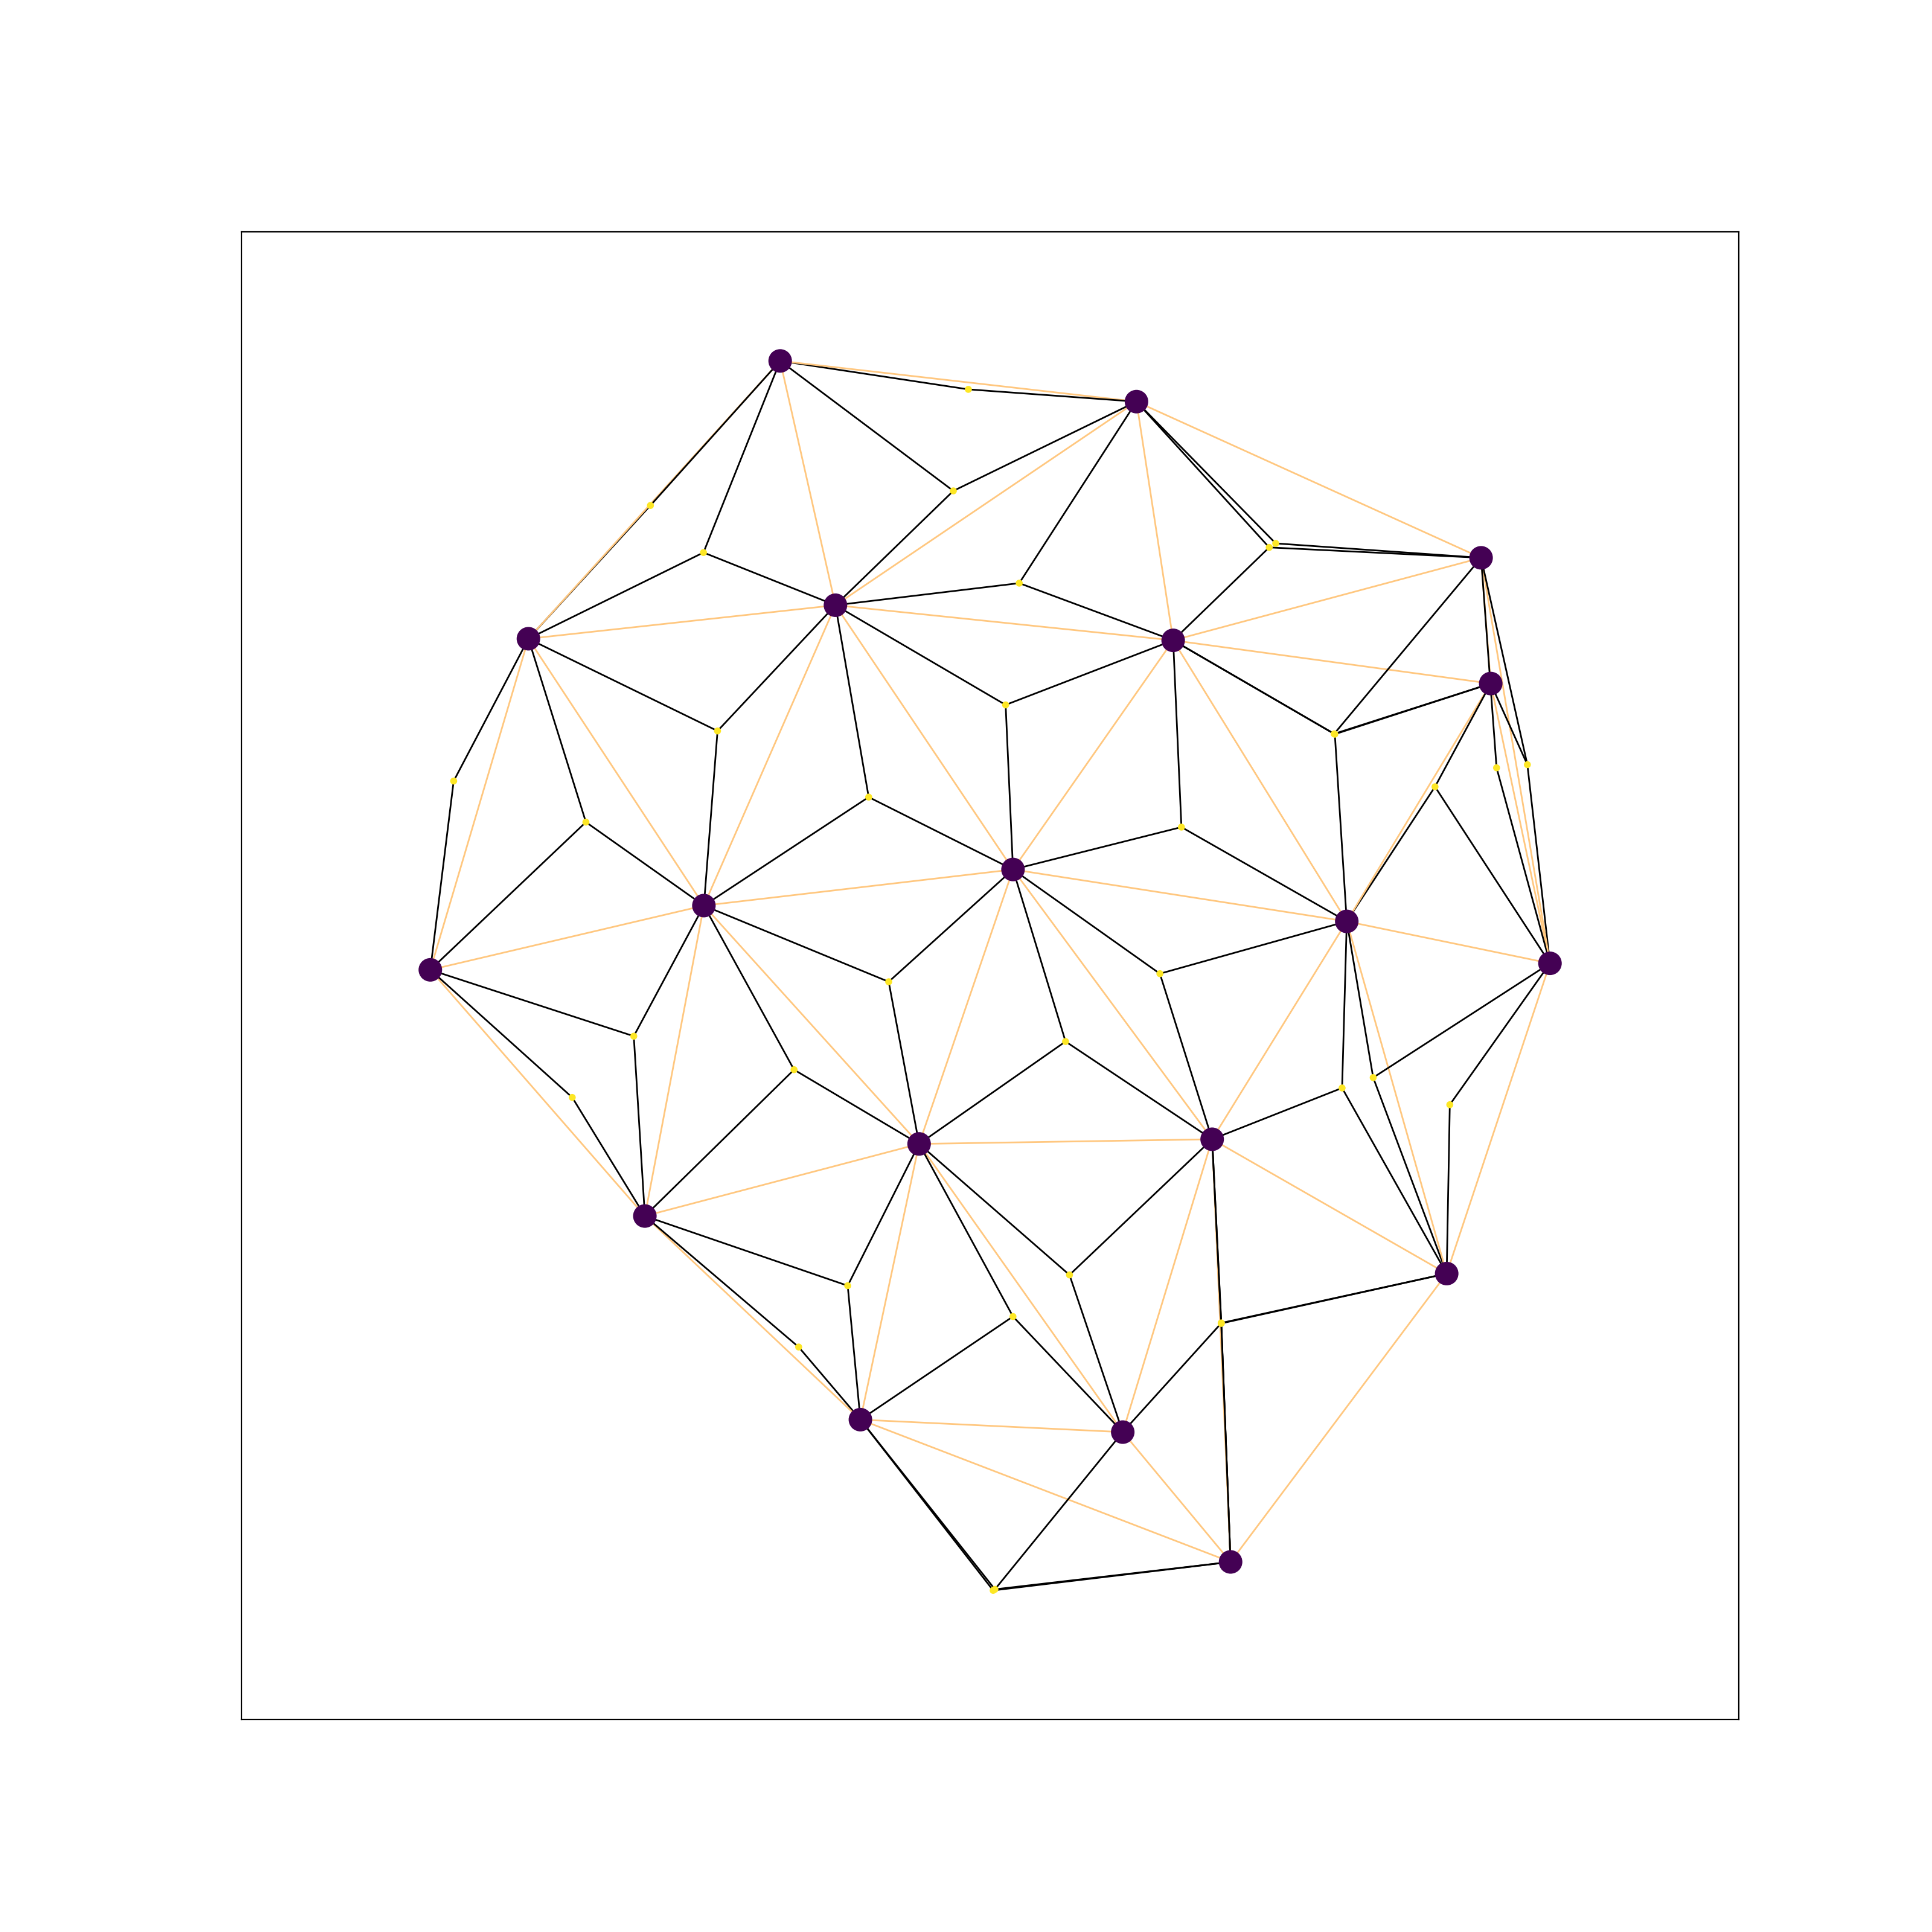
\includegraphics[width=0.3\textwidth]{figures/numerical/hexnoise/hexnoise0.8_0.8_1.52_10_graph.png}
        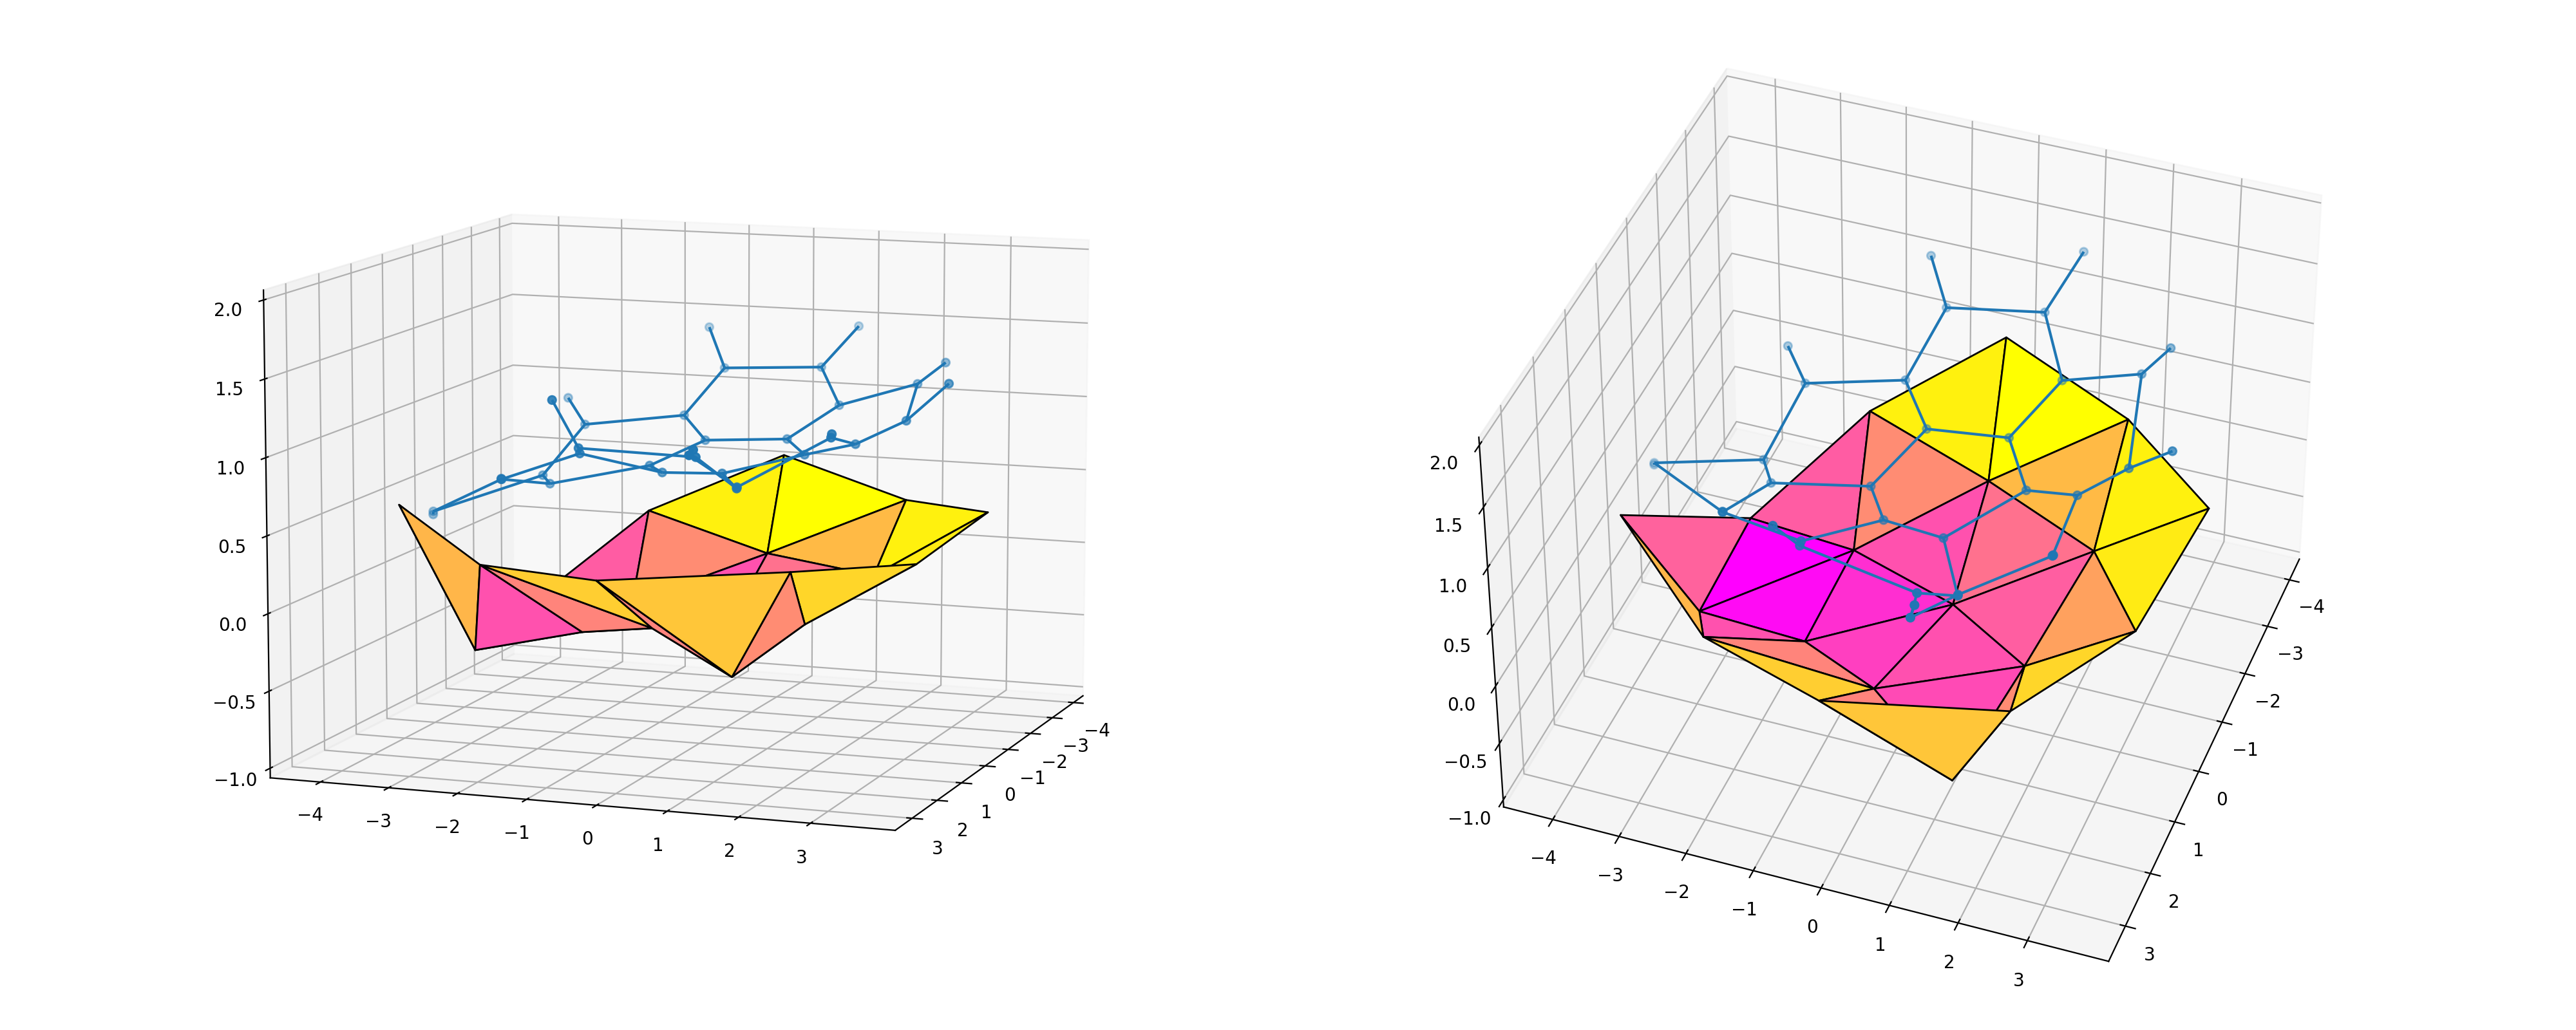
\includegraphics[width=0.69\textwidth]{figures/numerical/hexnoise/hexnoise0.8_0.8_1.52_10_plot.png}
        \caption{Sheet shape when $\phi_0=0.8$, $\psi_0=0.8$, $\ell_0=1.52$.}
        \label{subfig:hexnoise_in}
    \end{subfigure}
    \begin{subfigure}[b]{\textwidth}
        \centering
        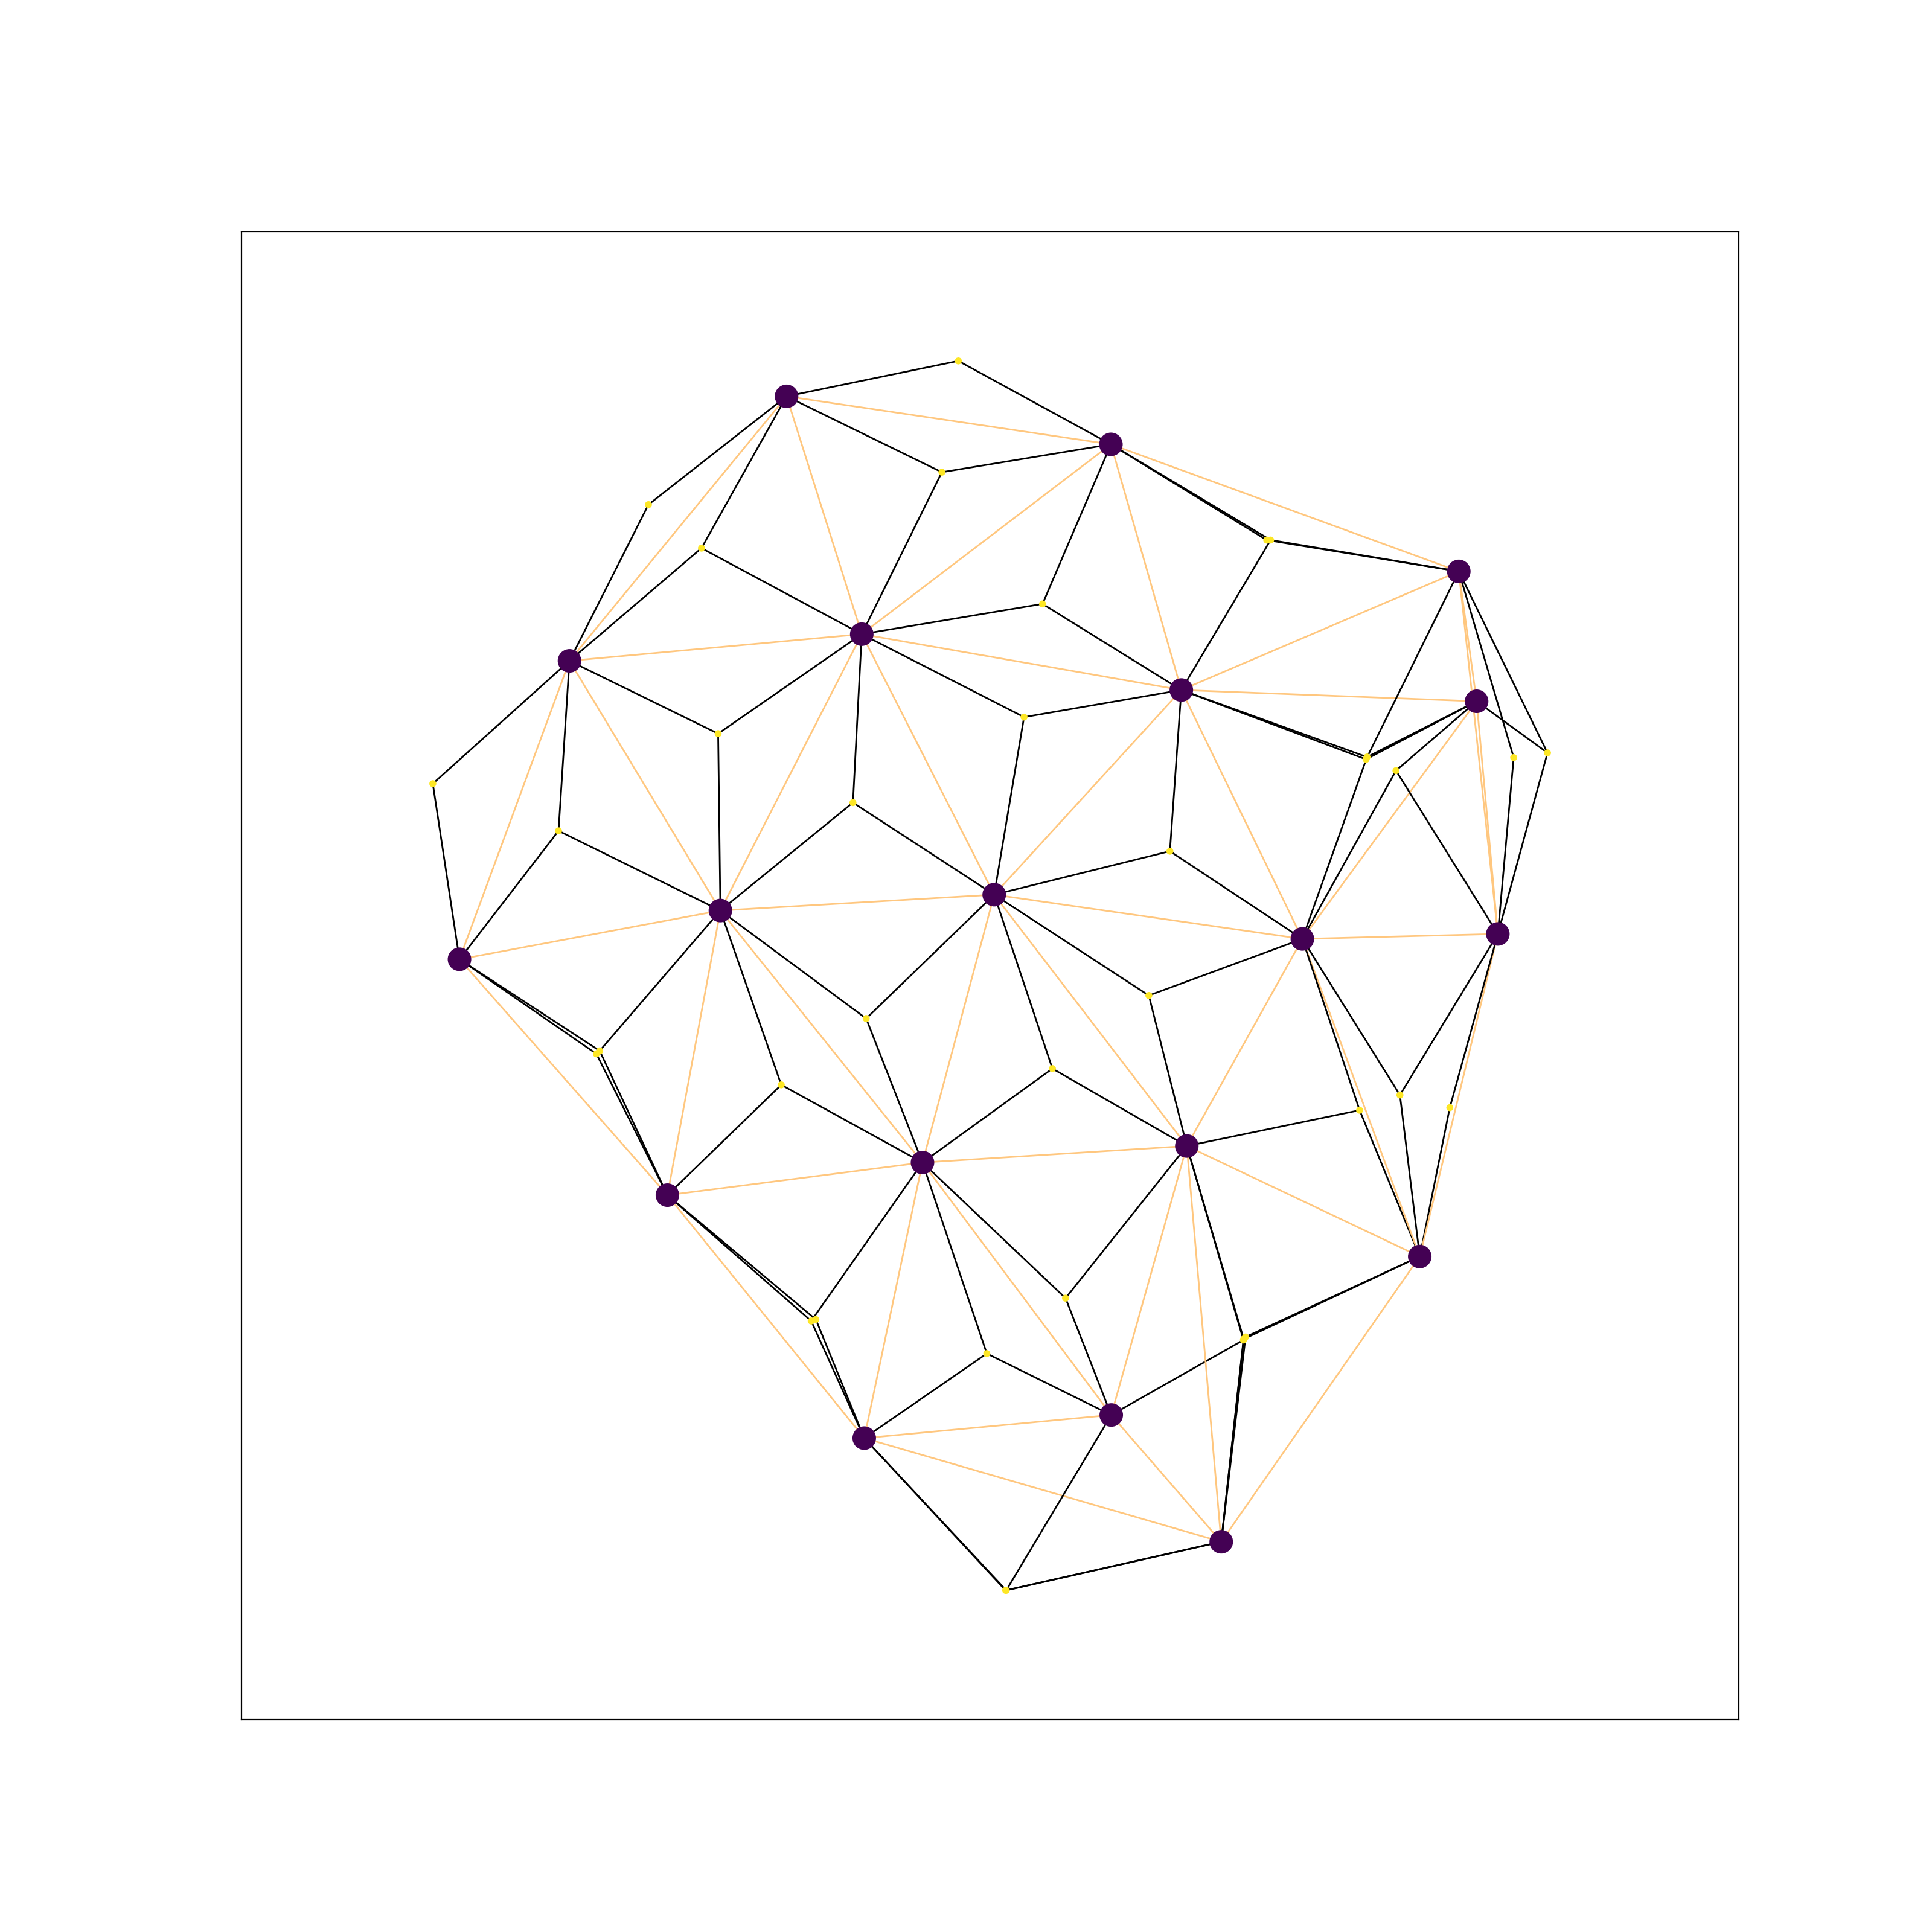
\includegraphics[width=0.3\textwidth]{figures/numerical/hexnoise/hexnoise0.95_0.8_1.52_10_graph.png}
        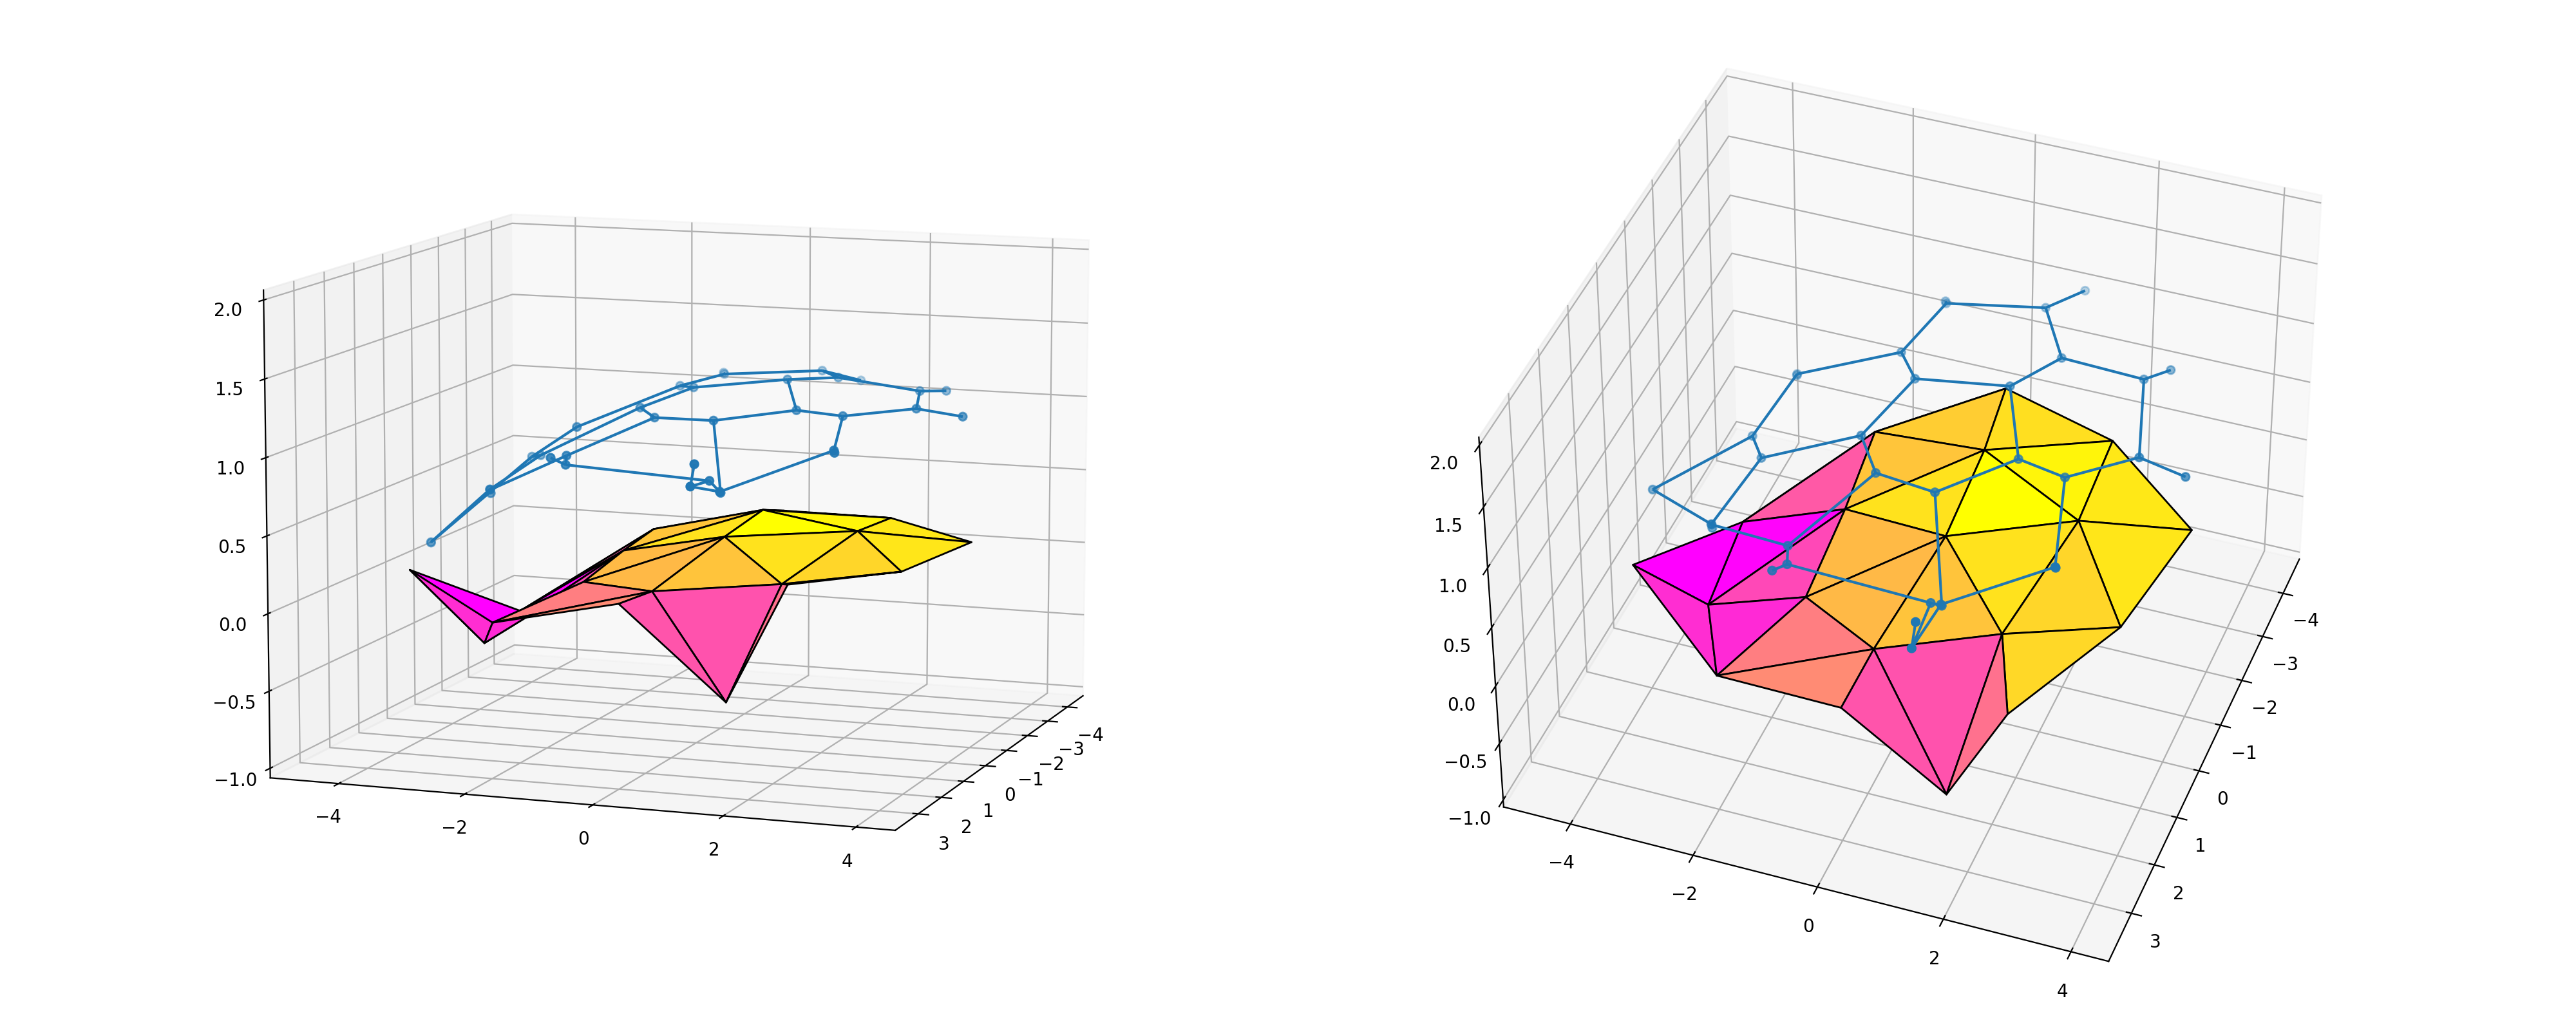
\includegraphics[width=0.69\textwidth]{figures/numerical/hexnoise/hexnoise0.95_0.8_1.52_10_plot.png}
        \caption{Sheet shape when $\phi_0=0.95$, $\psi_0=0.8$, $\ell_0=1.52$.}
        \label{subfig:hexnoise_out}
    \end{subfigure}
    \caption{Cell sheet geometry with noise added to the initial lattice. The graph topology is affected at the sheet boundary (subfigure \ref{subfig:hexnoise_graph}) from the Voronoi tesselation. This minor change has substantial effects on the sheet geometry (subfigures \ref{subfig:hexnoise_in}, \ref{subfig:hexnoise_out}).}
    \label{fig:hexnoise}
\end{figure}

\subsubsection{Interior cell topology}

We can also add or merge nodes in a regular lattice (Figure \ref{fig:layout_init}) to introduce nodes with irregular degree. There are more complex ways of making different graph topologies (like Lloyd's initial icosphere) but I don't have curved initial conditions or more complicated lattices implemented yet. 

Figure \ref{fig:kink} shows a sheet with cell of degree 7 (7 bordering cells) and \ref{fig:bump} shows a sheet with two neighboring cells of degree 5. 

\begin{figure}[htbp]
    \centering
    \begin{subfigure}[b]{\textwidth}
        \centering
        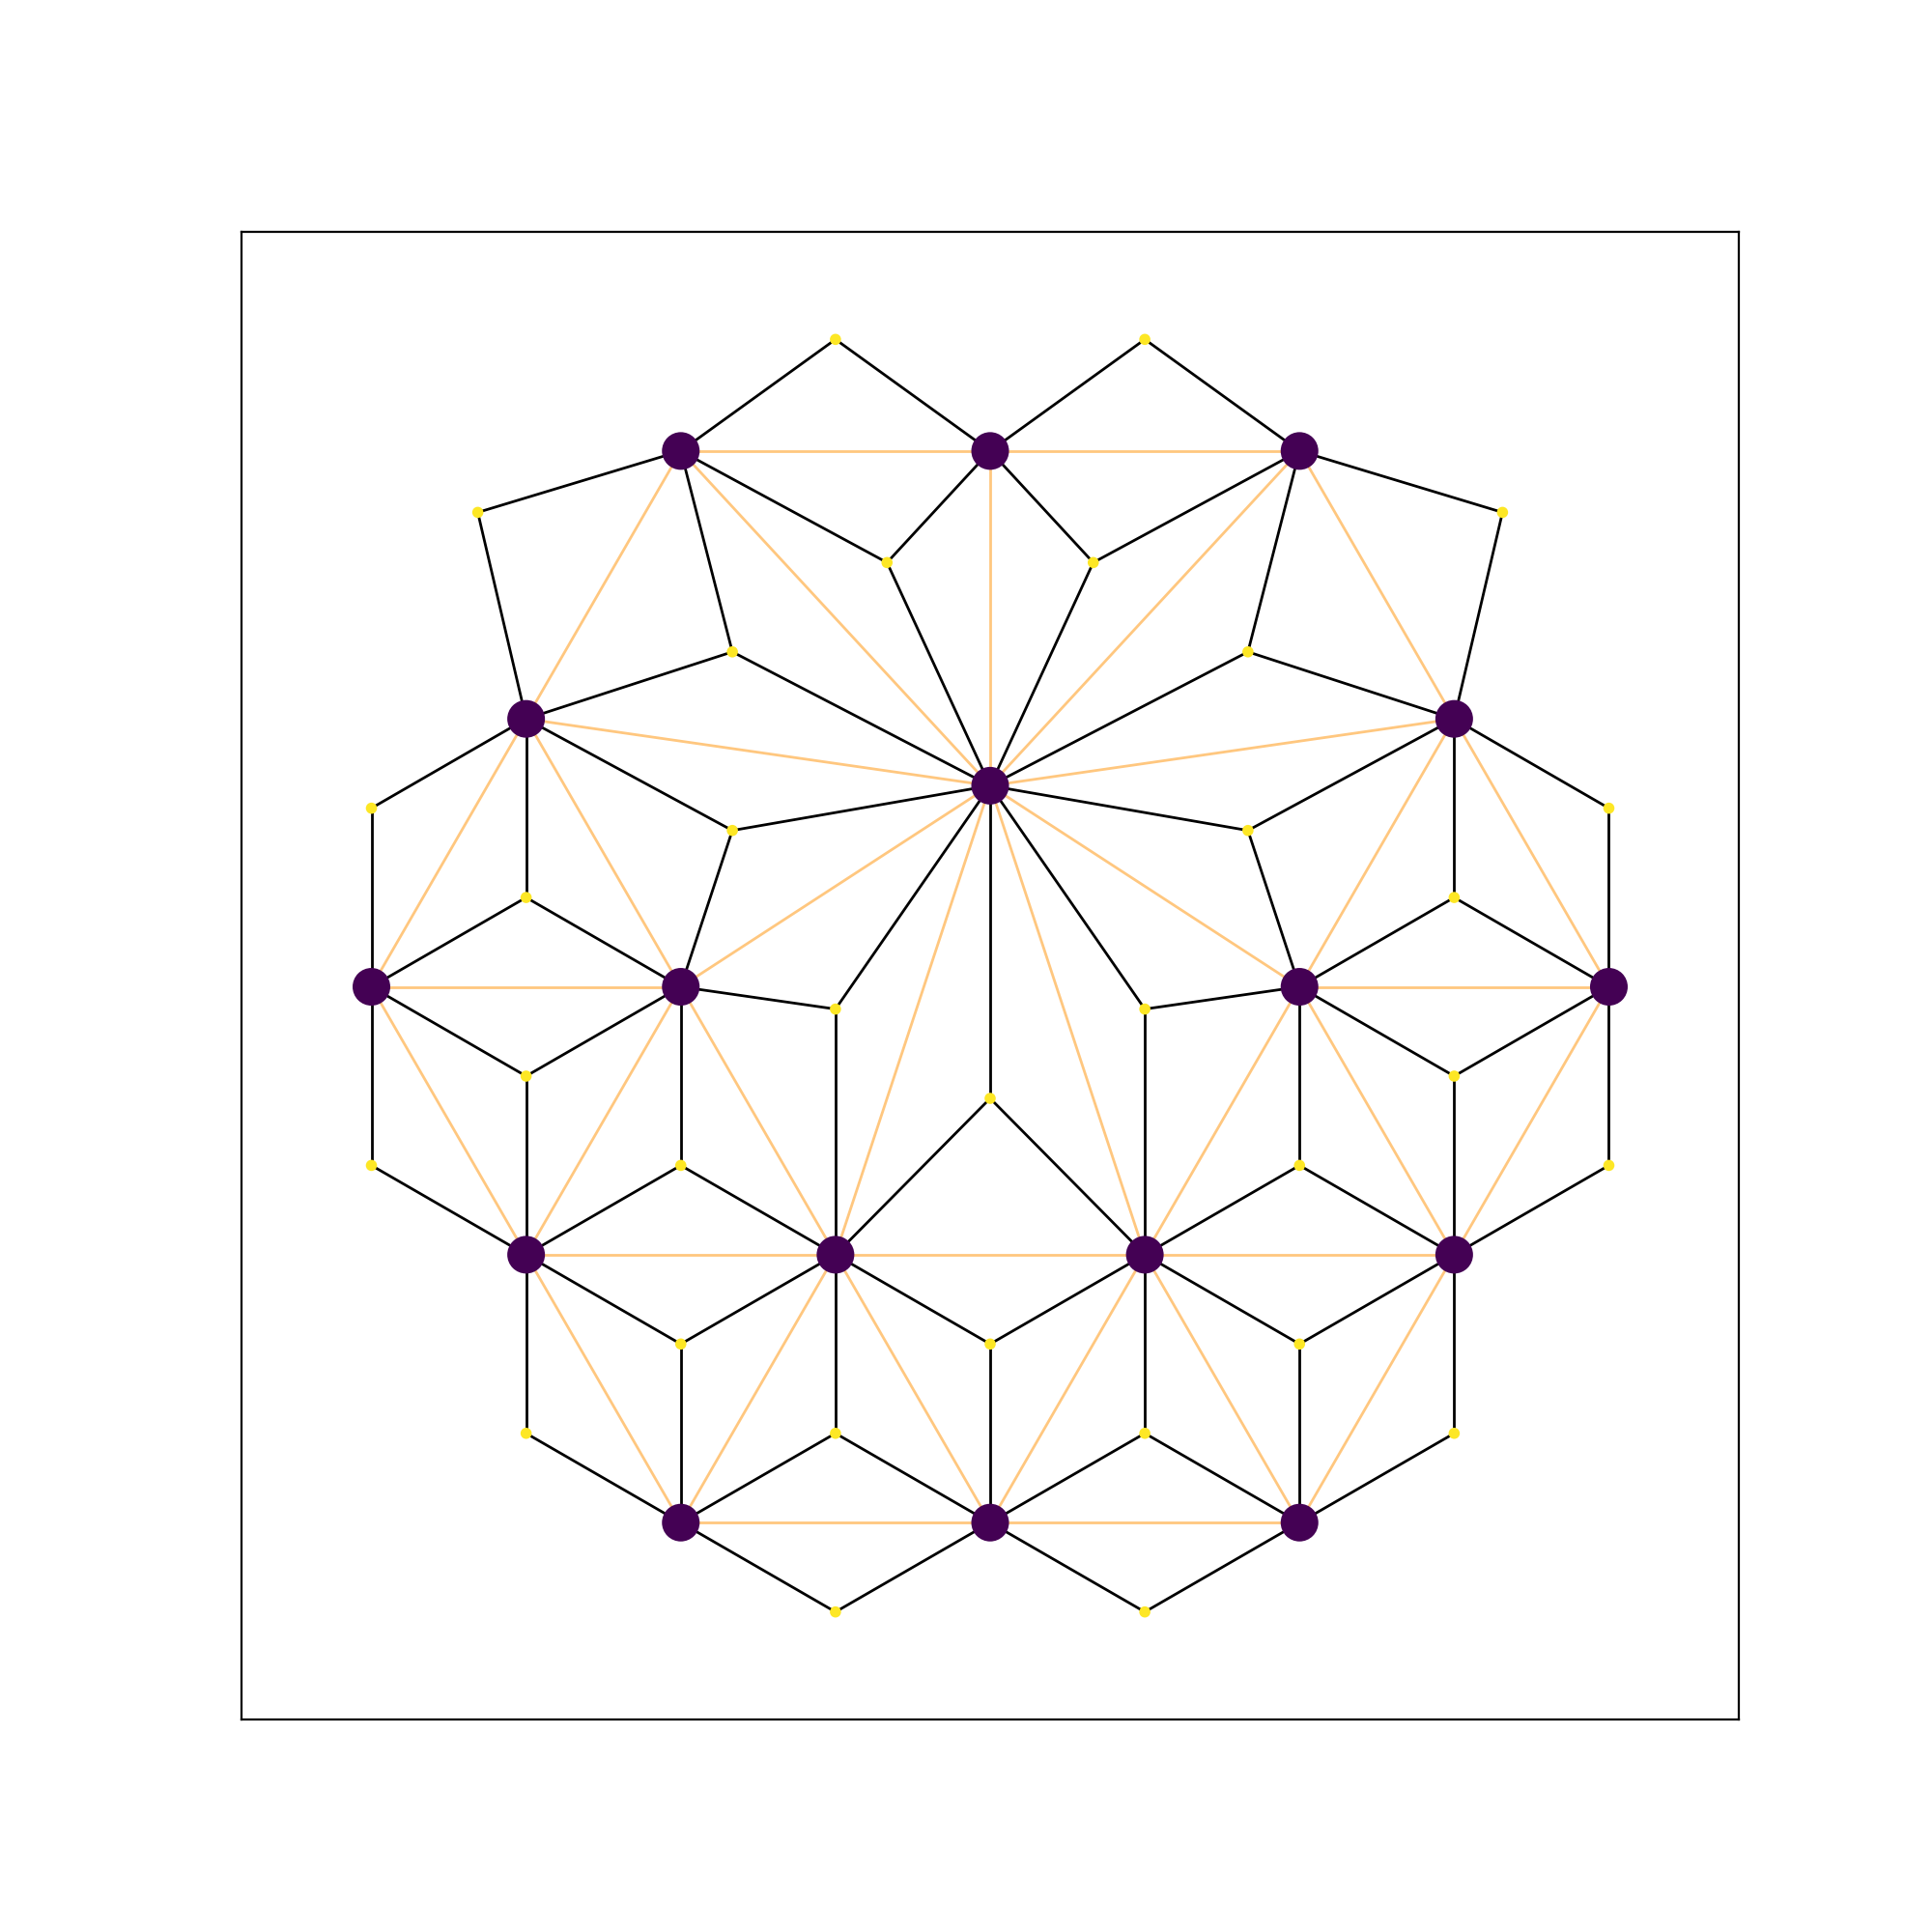
\includegraphics[width=0.5\textwidth]{figures/numerical/kink/kink_graph.png}
        \caption{Initial lattice drawn as in Figure \ref{fig:layout_init}.}
        \label{subfig:kink_graph}
    \end{subfigure}
    \begin{subfigure}[b]{\textwidth}
        \centering
        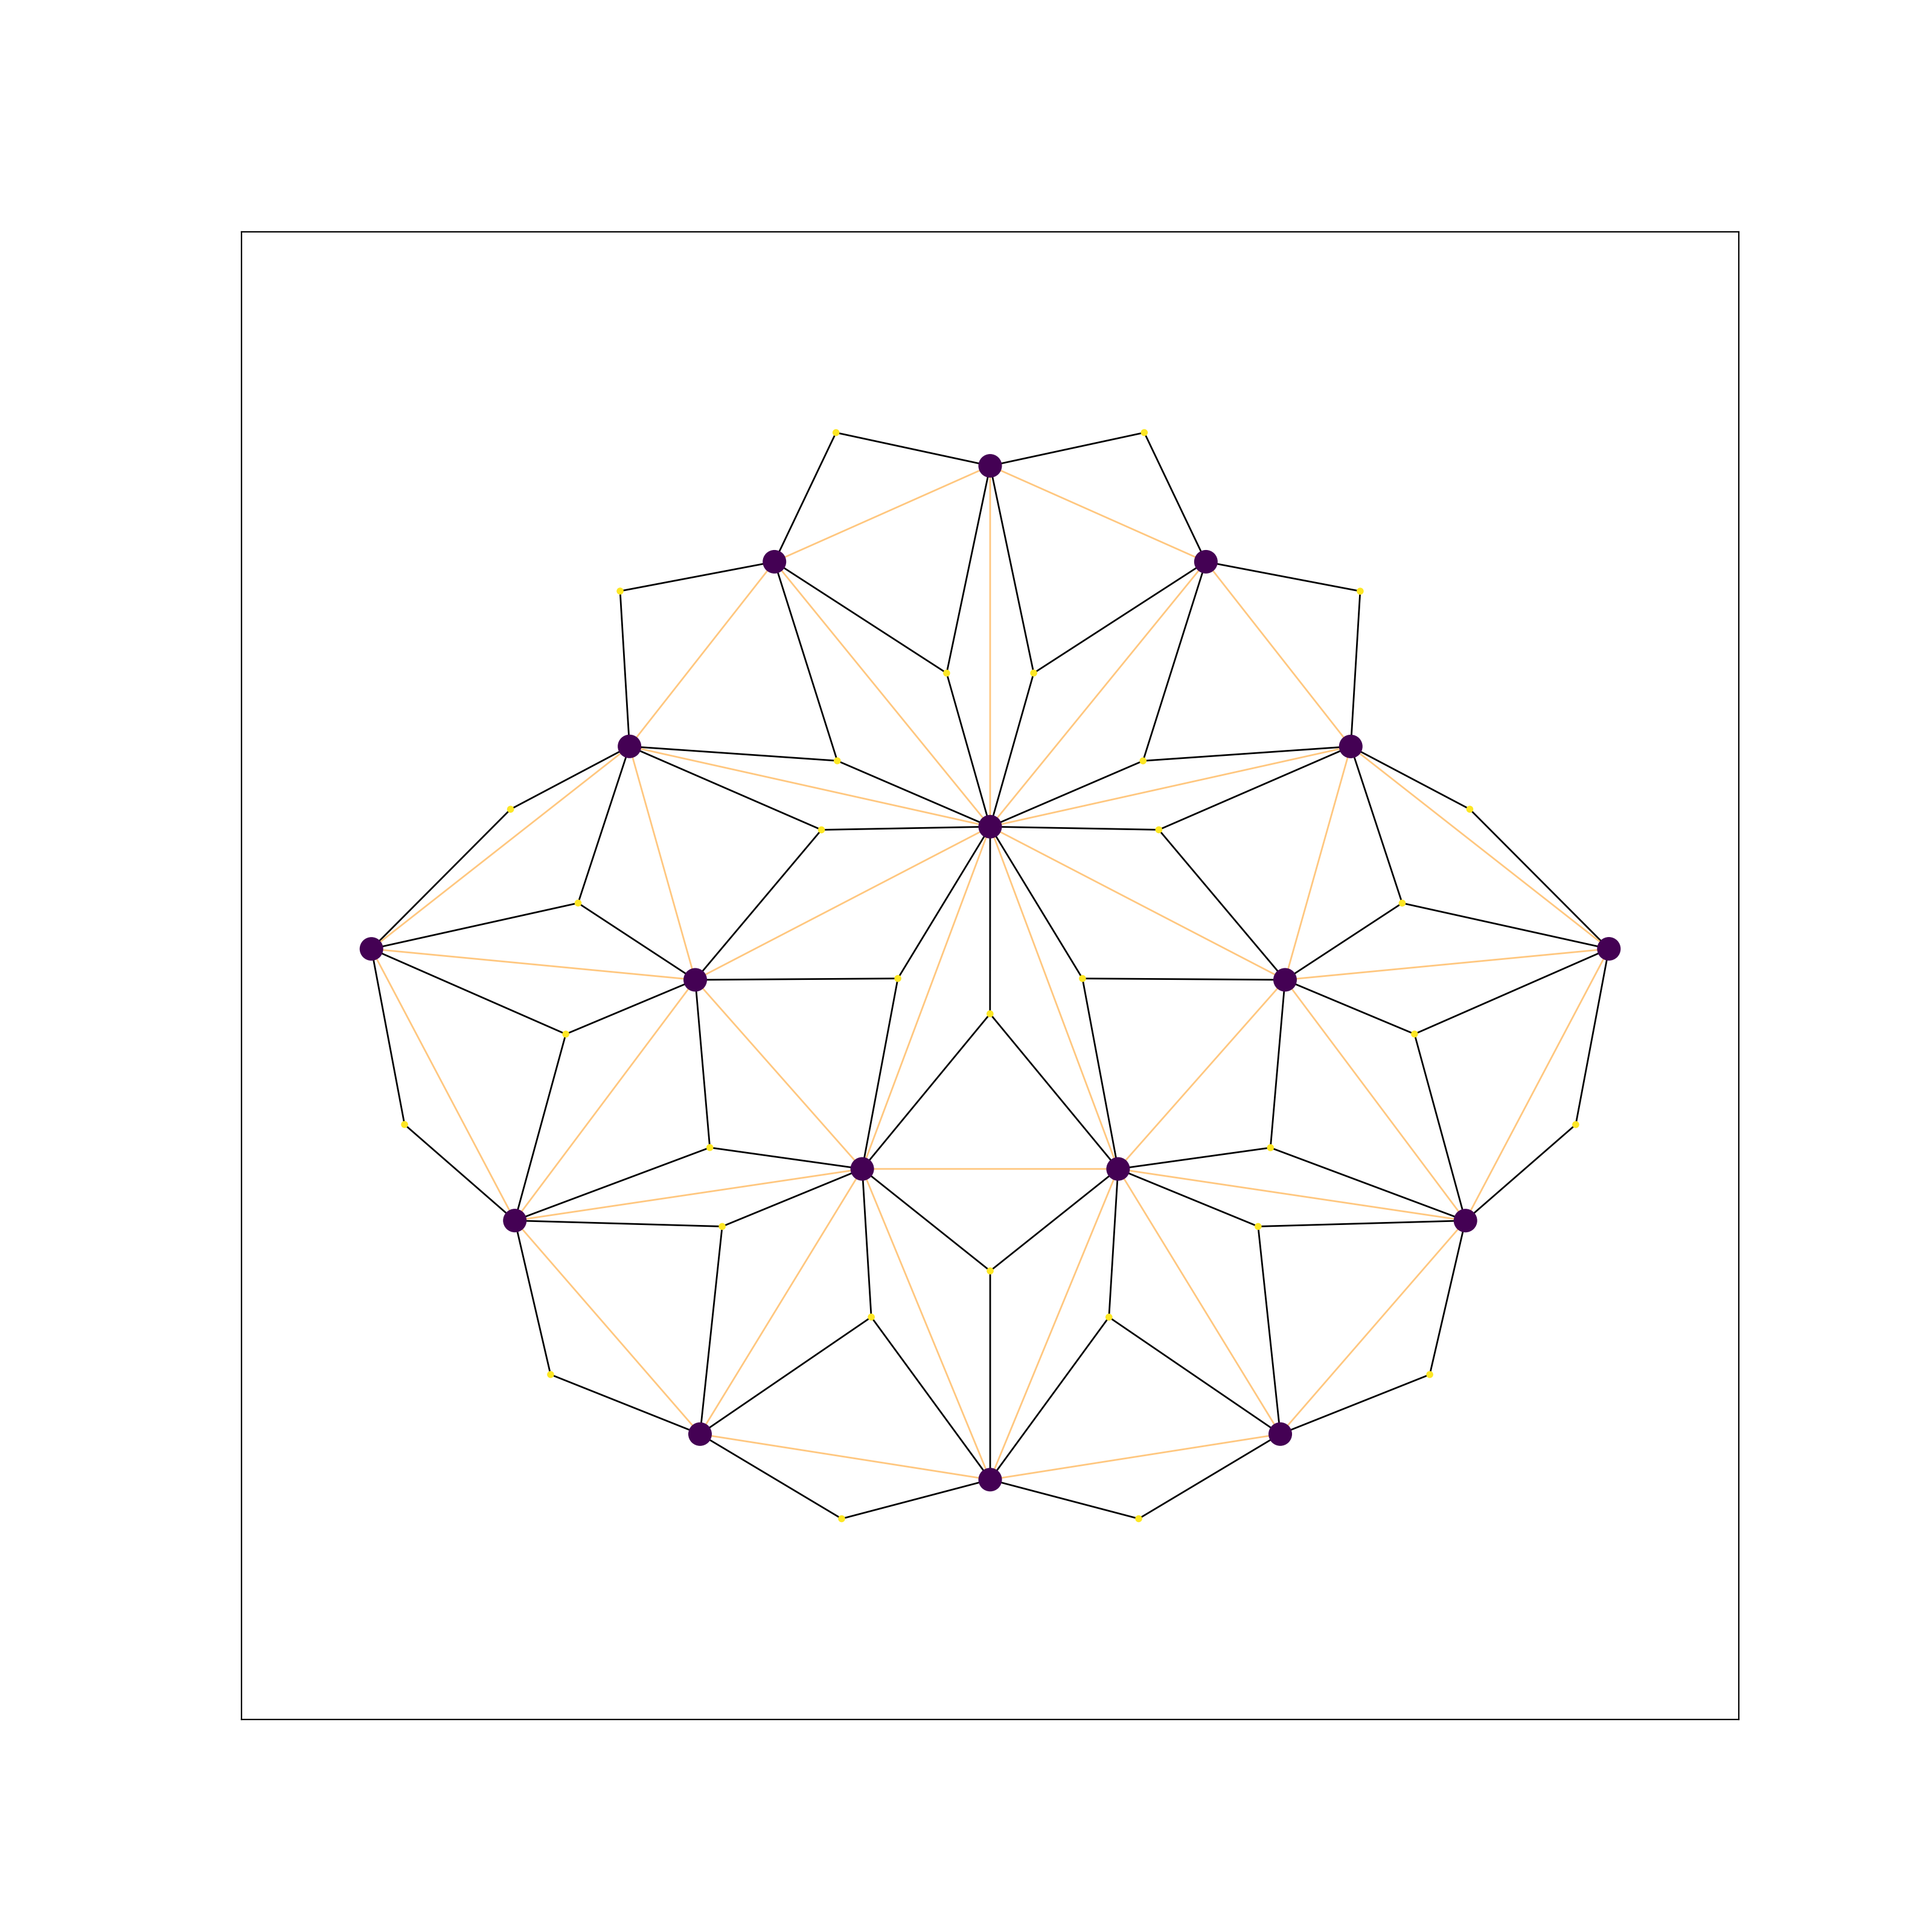
\includegraphics[width=0.3\textwidth]{figures/numerical/kink/kink0.8_0.8_1.52_10_graph.png}
        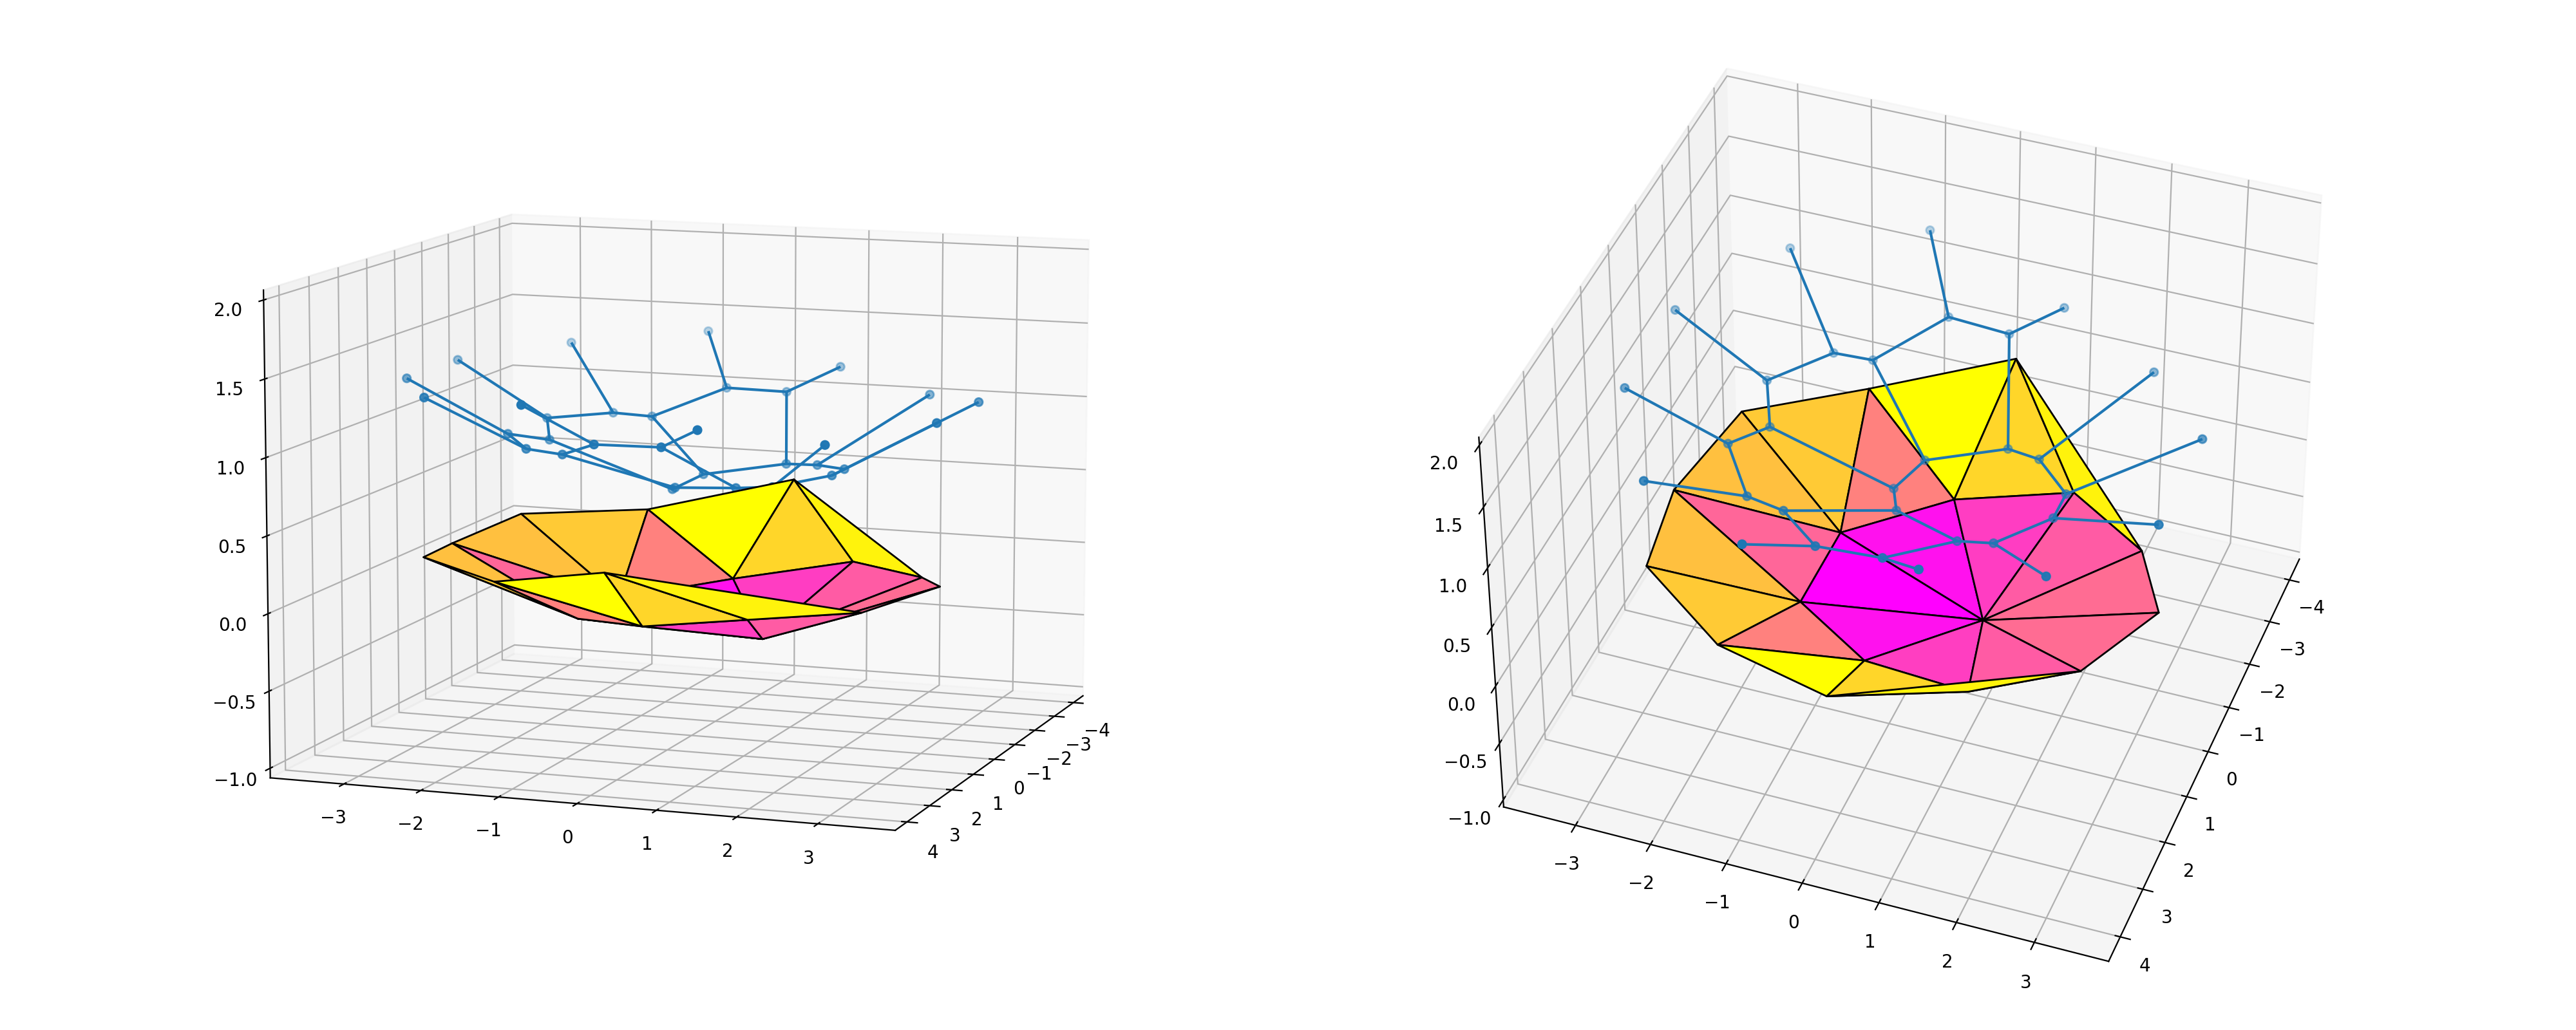
\includegraphics[width=0.69\textwidth]{figures/numerical/kink/kink0.8_0.8_1.52_10_plot.png}
        \caption{Sheet shape when $\phi_0=0.8$, $\psi_0=0.8$, $\ell_0=1.52$.}
        \label{subfig:kink_in}
    \end{subfigure}
    \begin{subfigure}[b]{\textwidth}
        \centering
        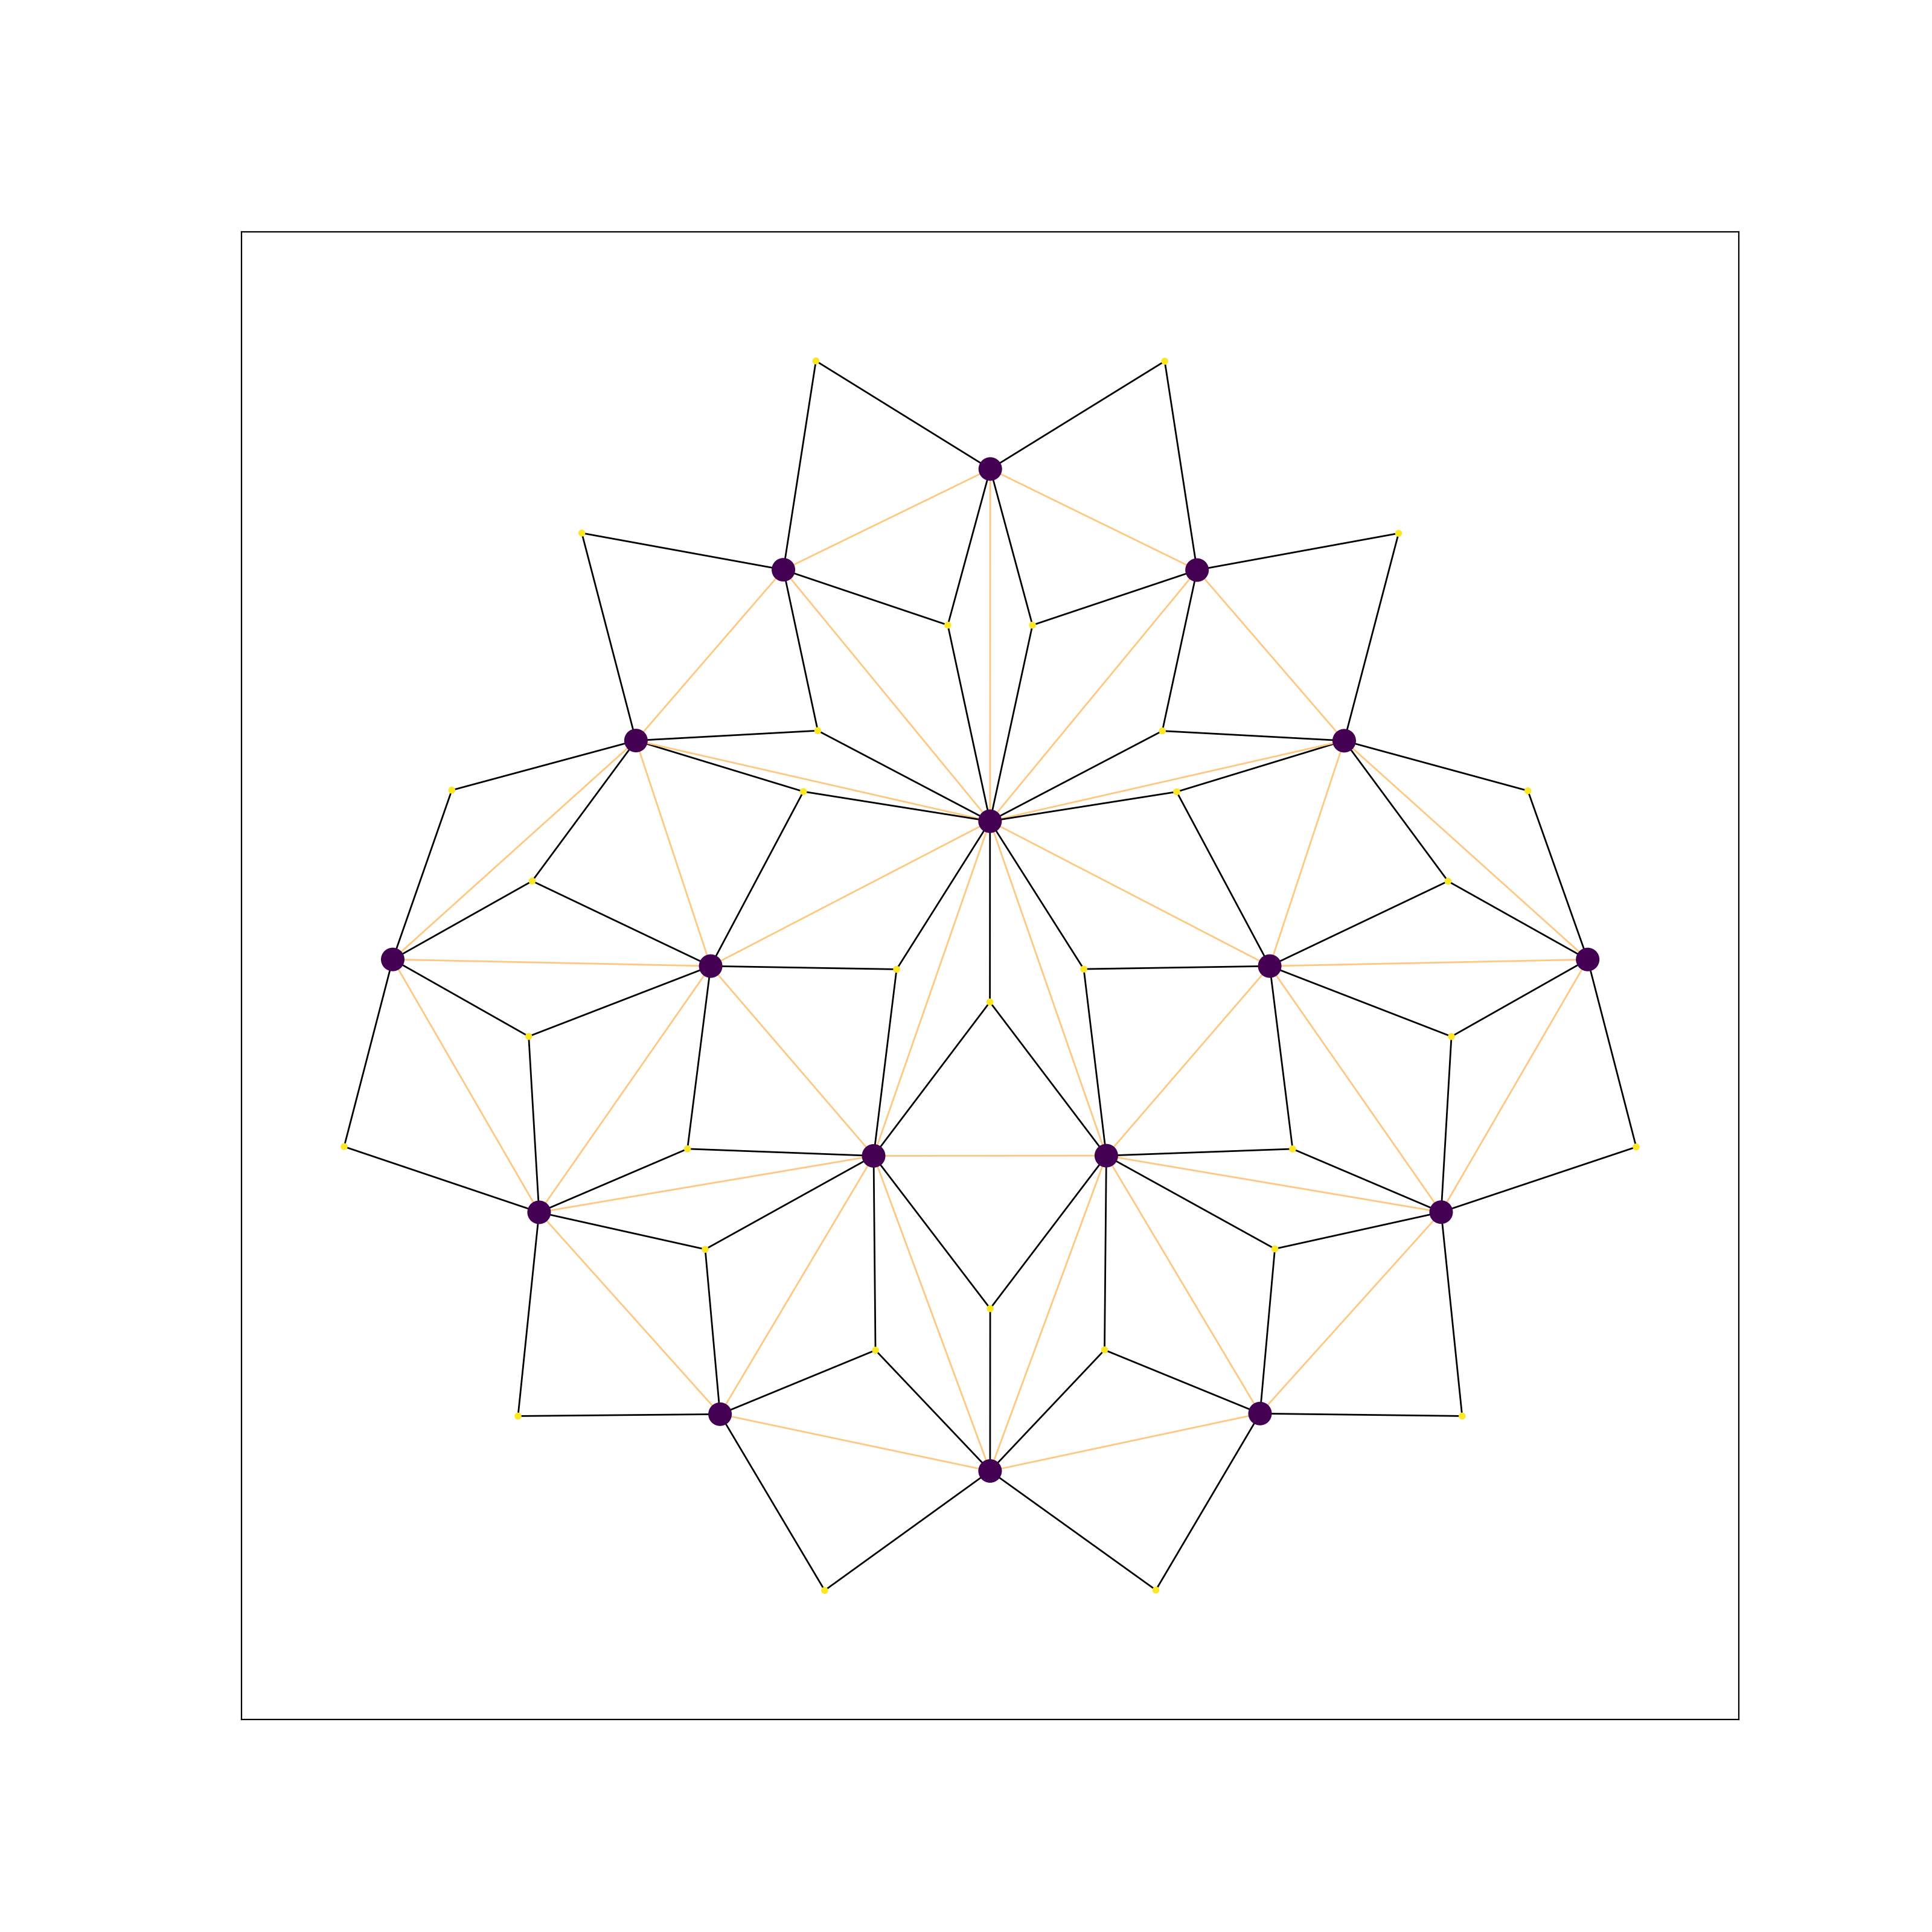
\includegraphics[width=0.3\textwidth]{figures/numerical/kink/kink0.95_0.8_1.52_10_graph.png}
        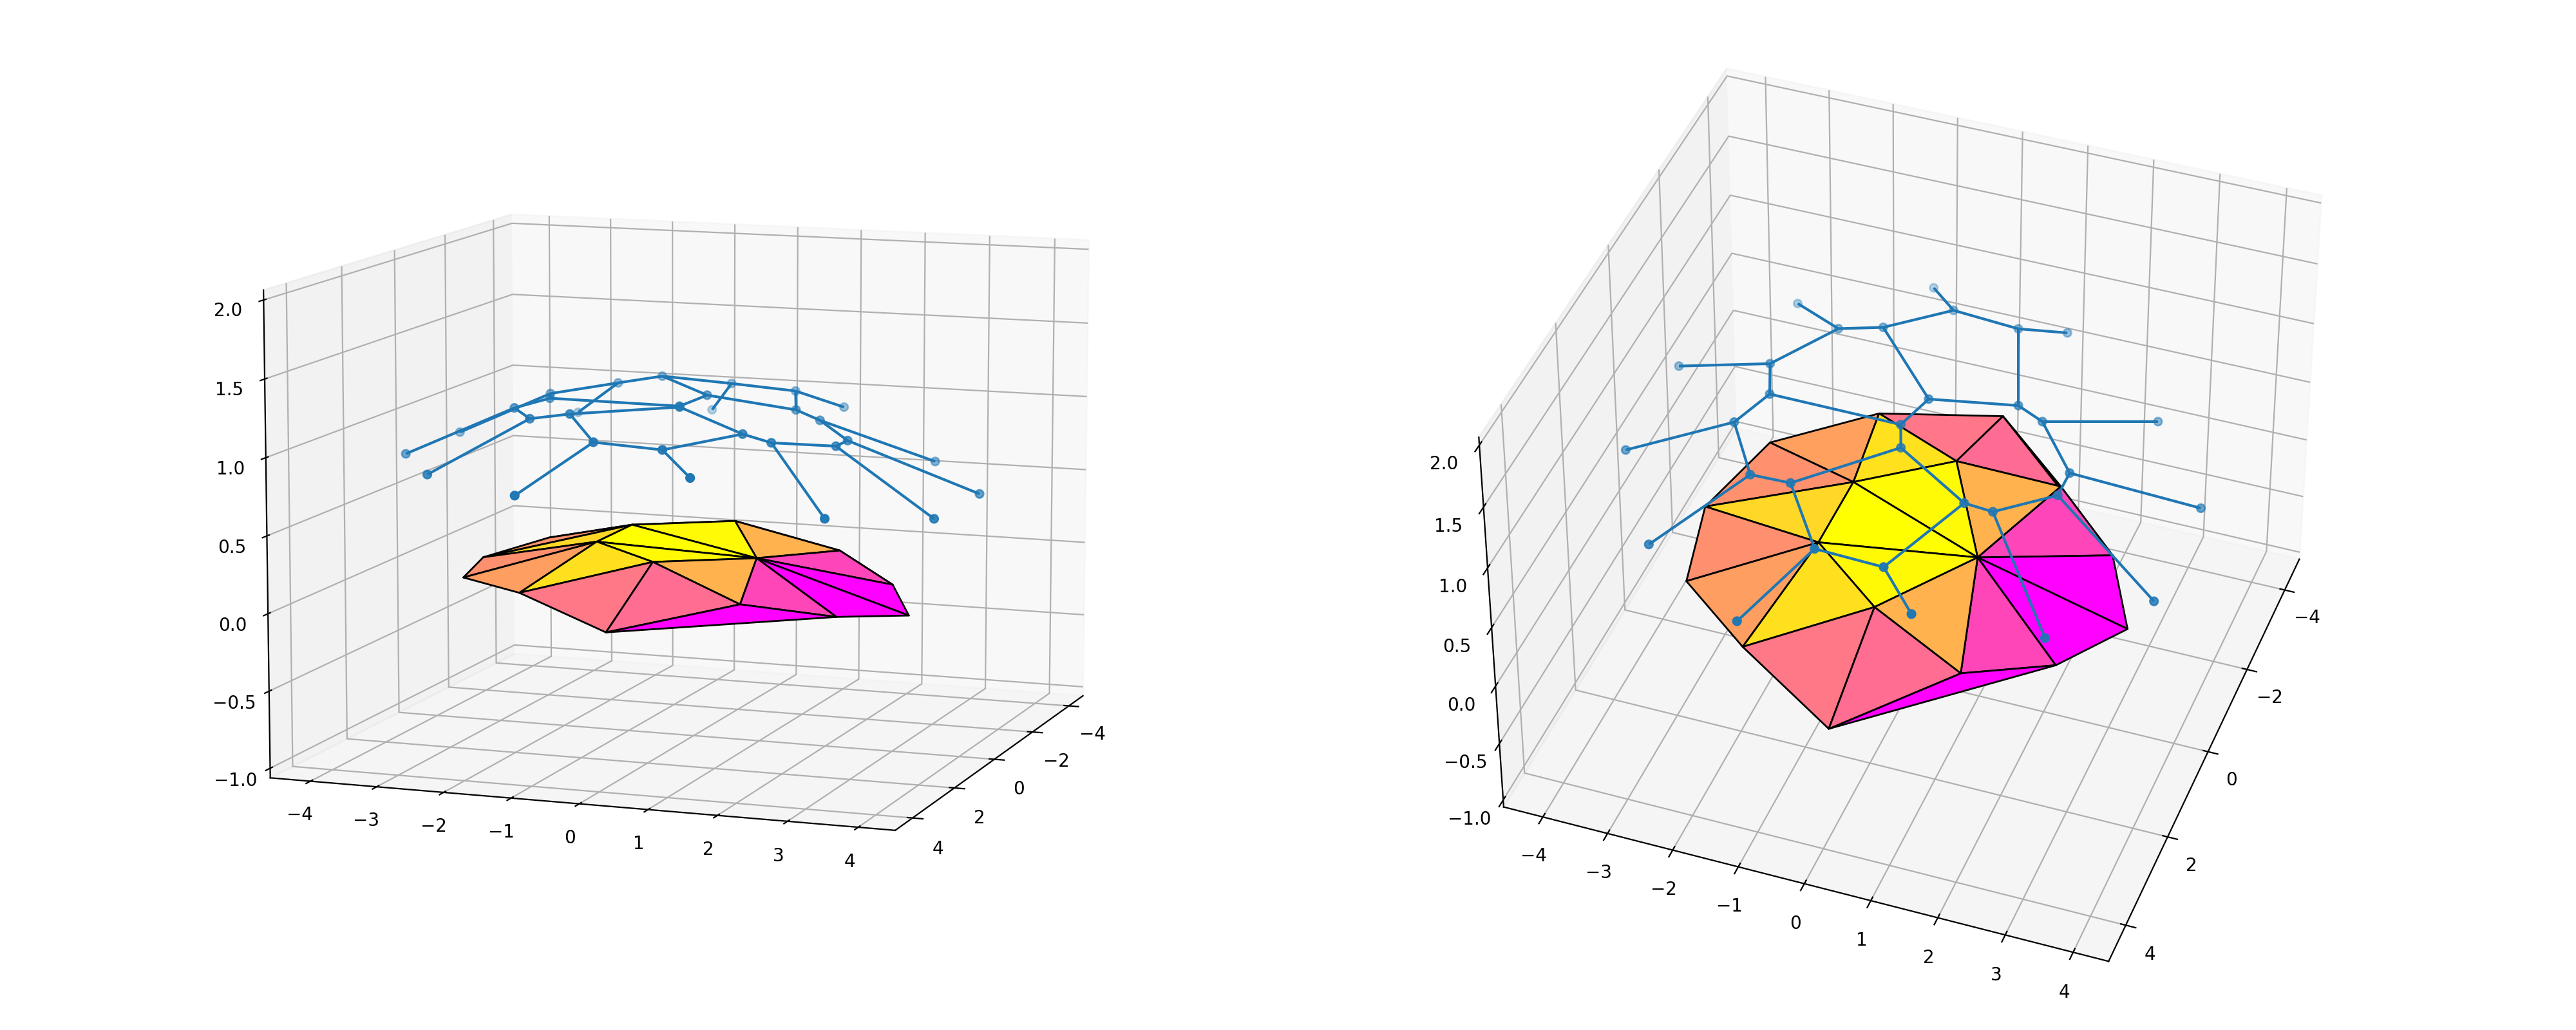
\includegraphics[width=0.69\textwidth]{figures/numerical/kink/kink0.95_0.8_1.52_10_plot.png}
        \caption{Sheet shape when $\phi_0=0.95$, $\psi_0=0.8$, $\ell_0=1.52$.}
        \label{subfig:kink_out}
    \end{subfigure}
    \caption{Cell sheet geometry with a node of degree 7. The graph topology is affected in the sheet interior (subfigure \ref{subfig:kink_graph}). This minor change has substantial effects on the sheet geometry (subfigures \ref{subfig:kink_in}, \ref{subfig:kink_out}).}
    \label{fig:kink}
\end{figure}

\begin{figure}[htbp]
    \centering
    \begin{subfigure}[b]{\textwidth}
        \centering
        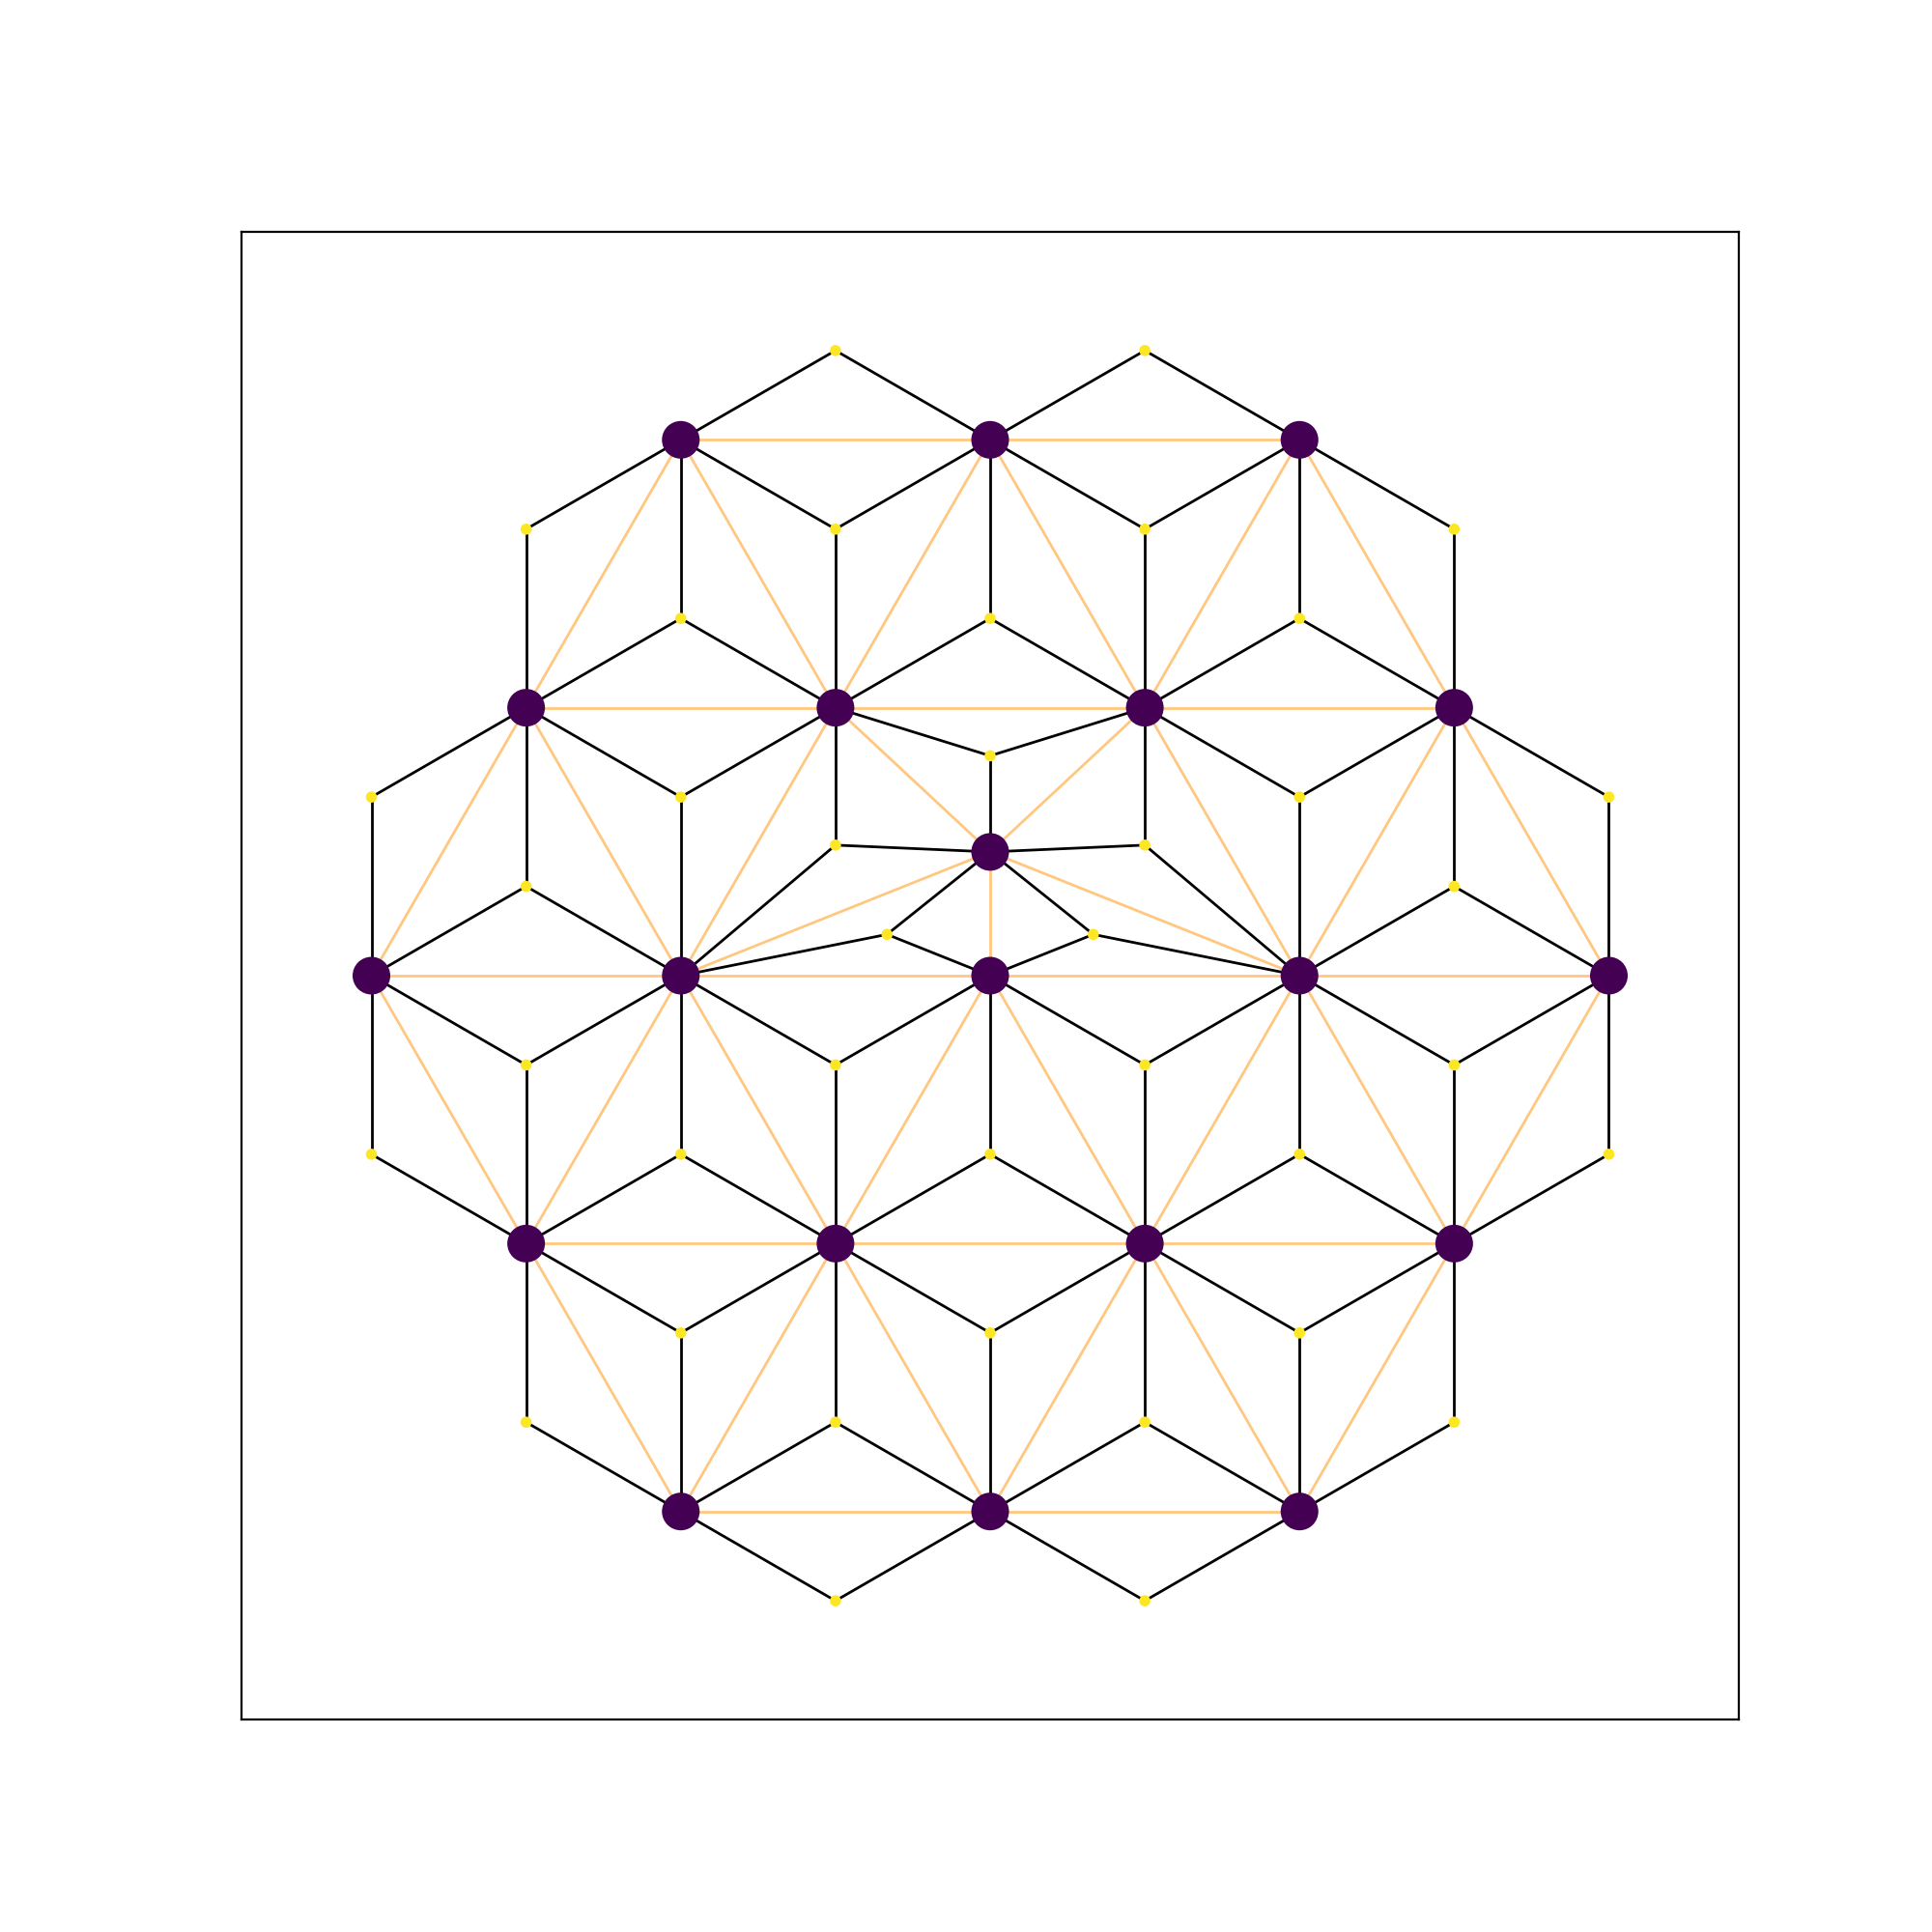
\includegraphics[width=0.5\textwidth]{figures/numerical/bump/bump_graph.png}
        \caption{Initial lattice drawn as in Figure \ref{fig:layout_init}.}
        \label{subfig:bump_graph}
    \end{subfigure}
    \begin{subfigure}[b]{\textwidth}
        \centering
        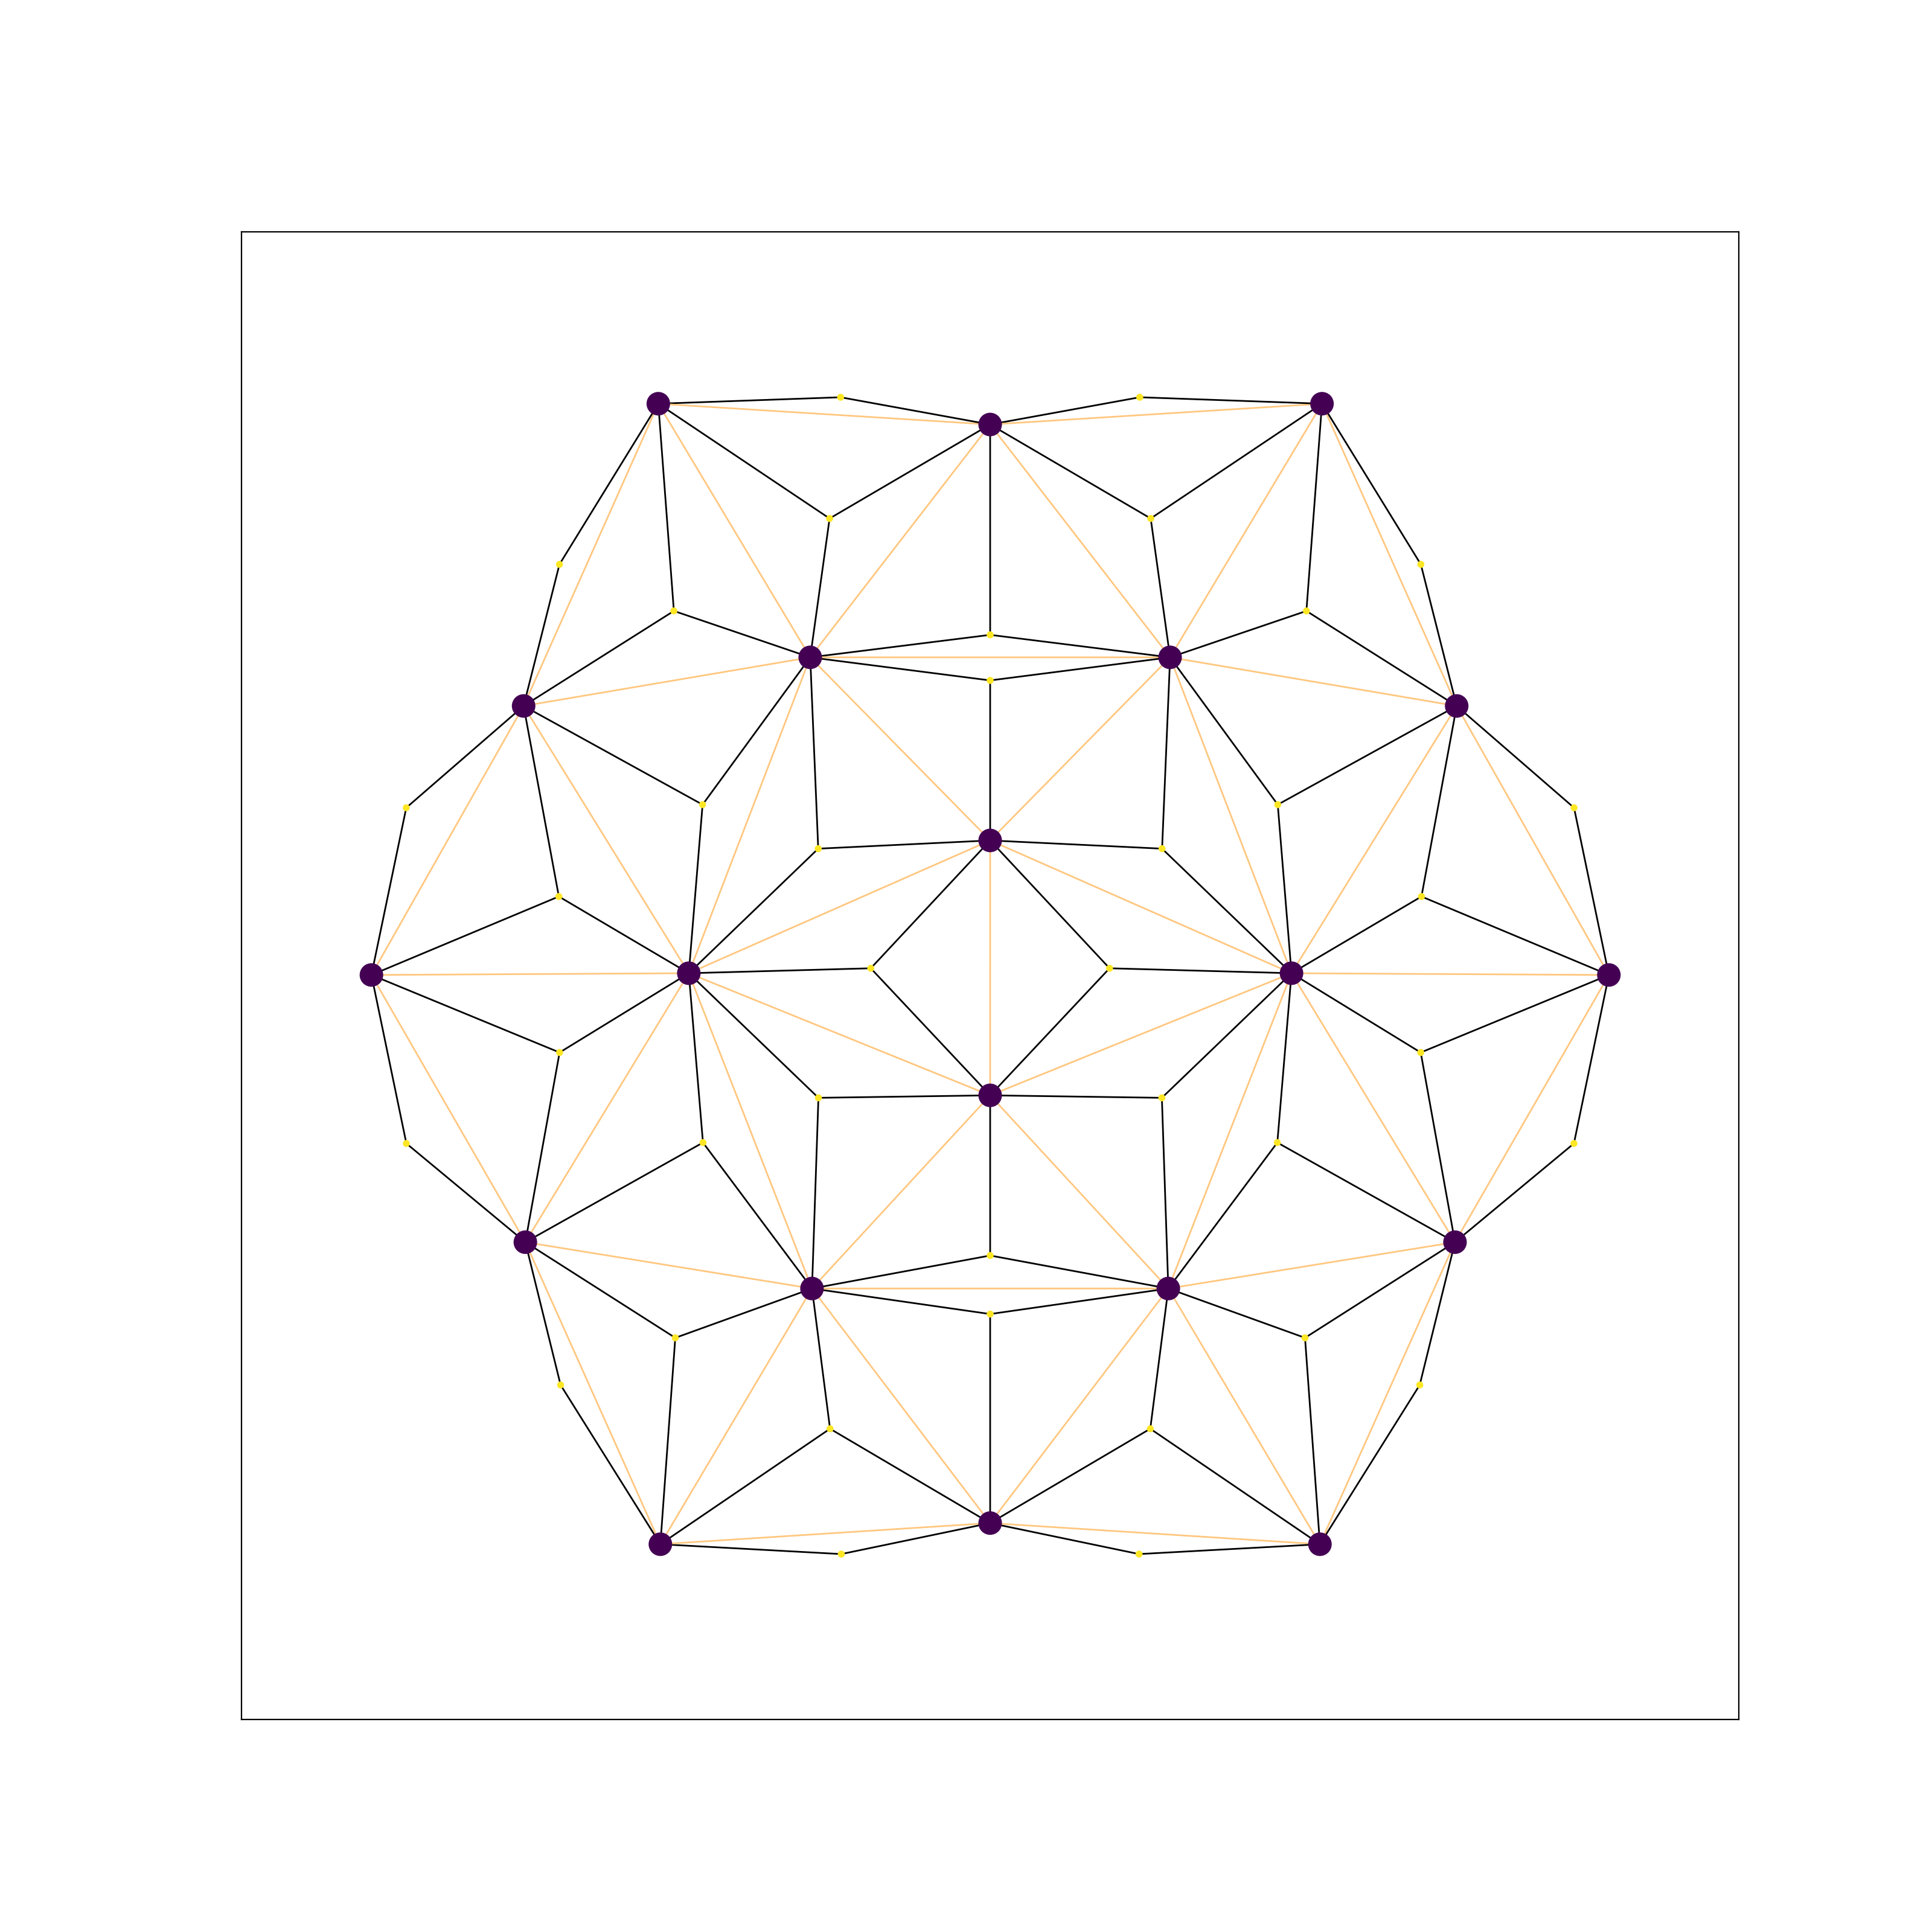
\includegraphics[width=0.3\textwidth]{figures/numerical/bump/bump0.8_0.8_1.52_10_graph.png}
        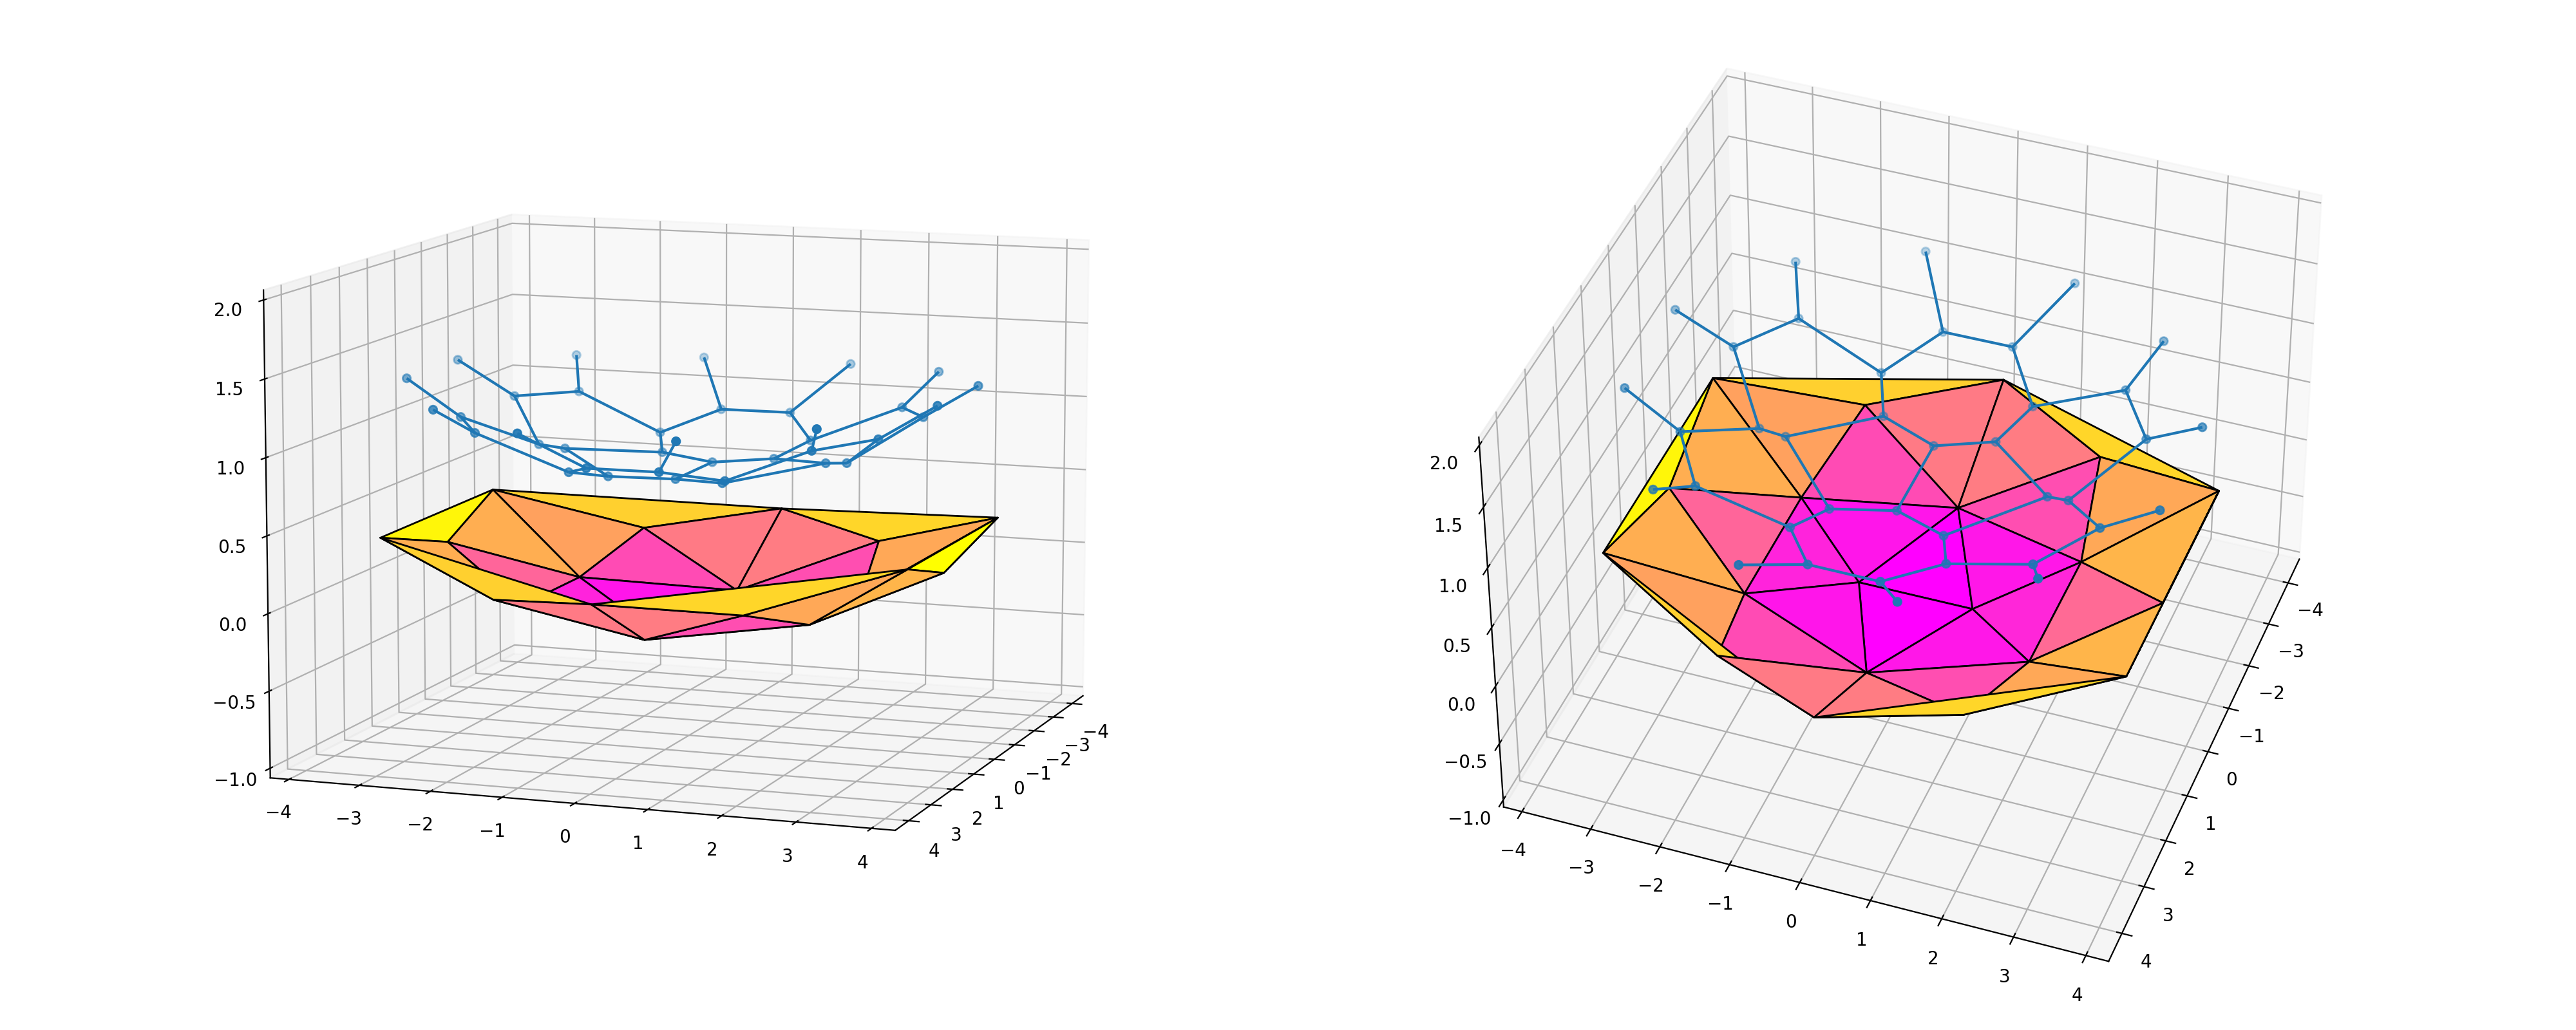
\includegraphics[width=0.69\textwidth]{figures/numerical/bump/bump0.8_0.8_1.52_10_plot.png}
        \caption{Sheet shape when $\phi_0=0.8$, $\psi_0=0.8$, $\ell_0=1.52$.}
        \label{subfig:bump_in}
    \end{subfigure}
    \begin{subfigure}[b]{\textwidth}
        \centering
        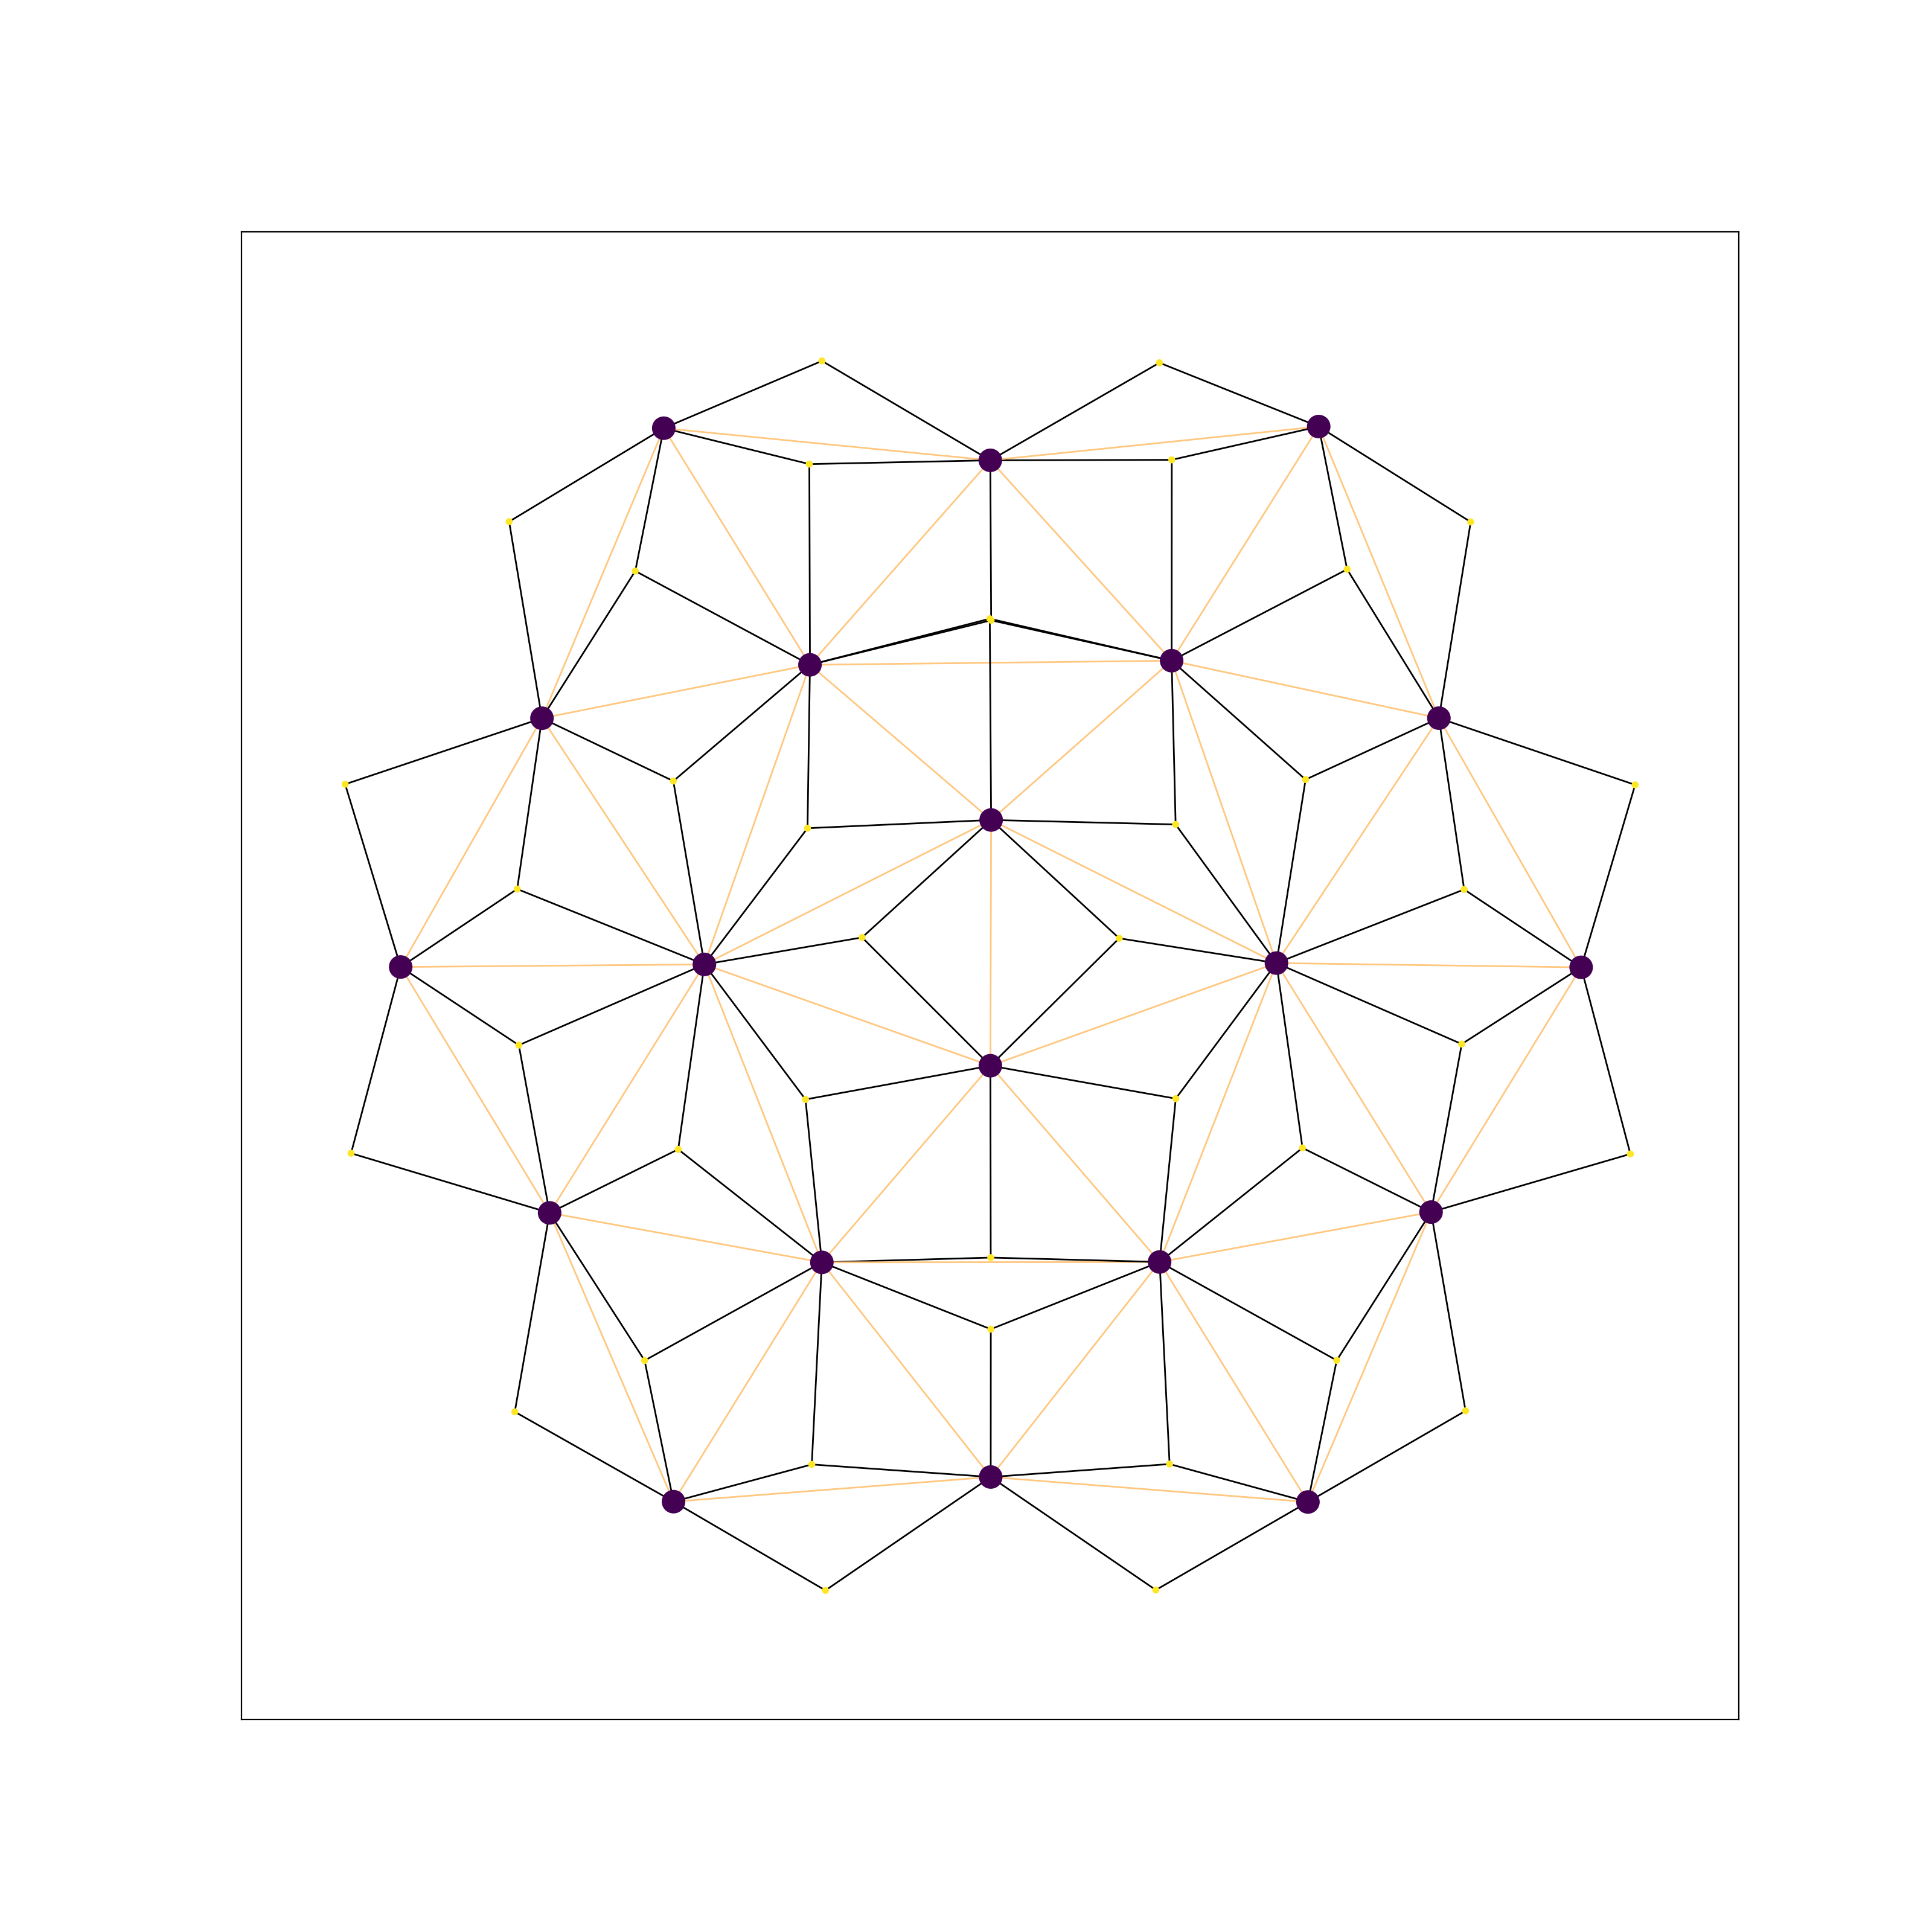
\includegraphics[width=0.3\textwidth]{figures/numerical/bump/bump0.95_0.8_1.52_10_graph.png}
        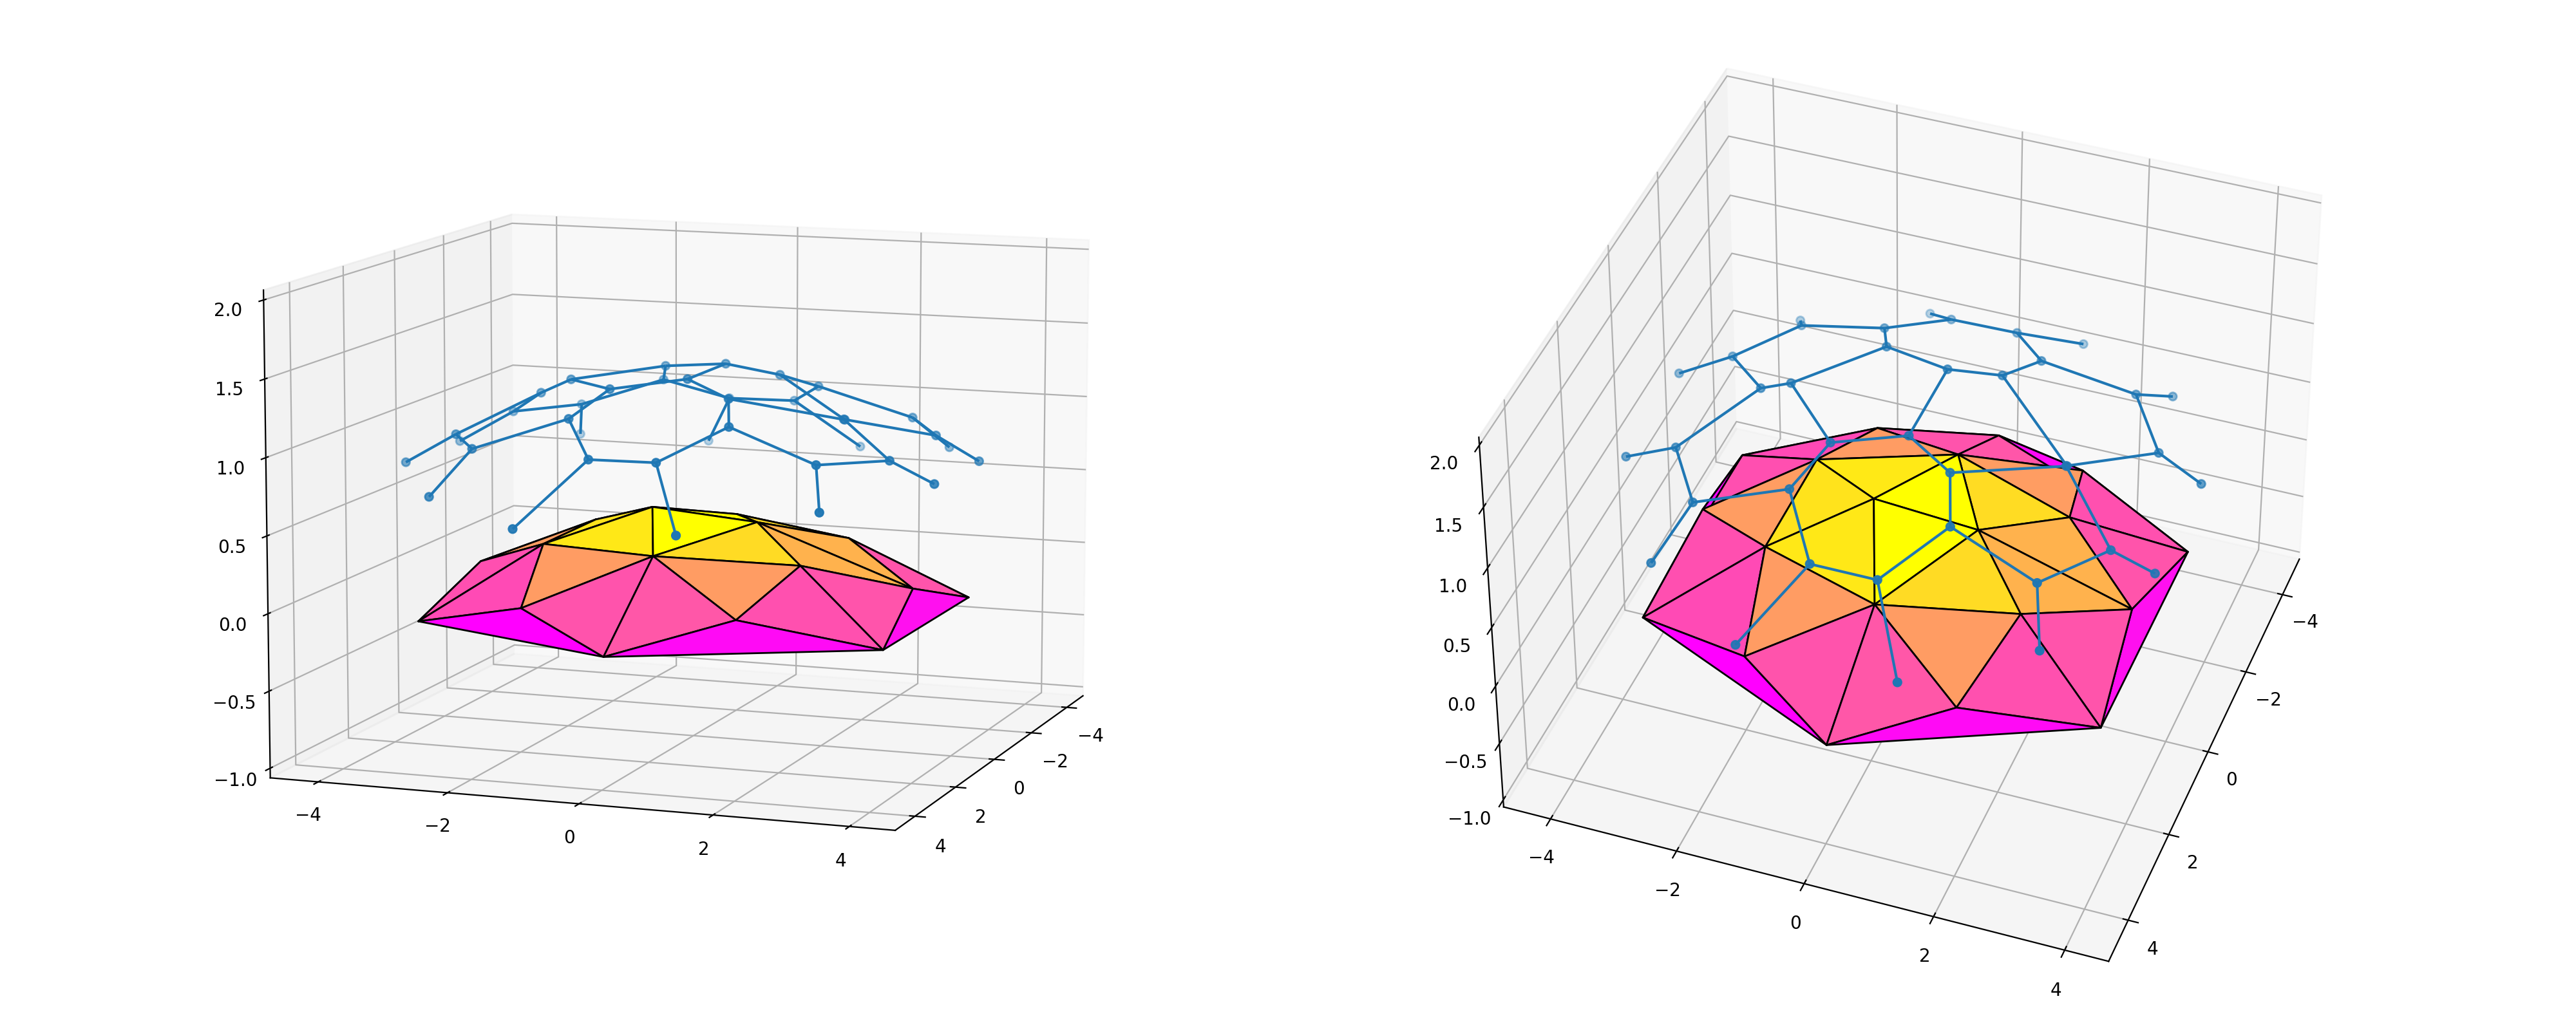
\includegraphics[width=0.69\textwidth]{figures/numerical/bump/bump0.95_0.8_1.52_10_plot.png}
        \caption{Sheet shape when $\phi_0=0.95$, $\psi_0=0.8$, $\ell_0=1.52$.}
        \label{subfig:bump_out}
    \end{subfigure}
    \caption{Cell sheet geometry with a node of degree 7. The graph topology is affected in the sheet interior (subfigure \ref{subfig:bump_graph}). This minor change has substantial effects on the sheet geometry (subfigures \ref{subfig:bump_in}, \ref{subfig:bump_out}).}
    \label{fig:bump}
\end{figure}

\subsection{Larger cell sheets}

If if inverting a sheet of cells involves flattening it out at the edges, then a small sheet will be able to do this easier than a large one. This is because the cells on the outside have to stretch their collars less if the sheet is smaller when they flatten out. 

\begin{figure}[htbp]
    \centering
    \begin{subfigure}[b]{\textwidth}
        \centering
        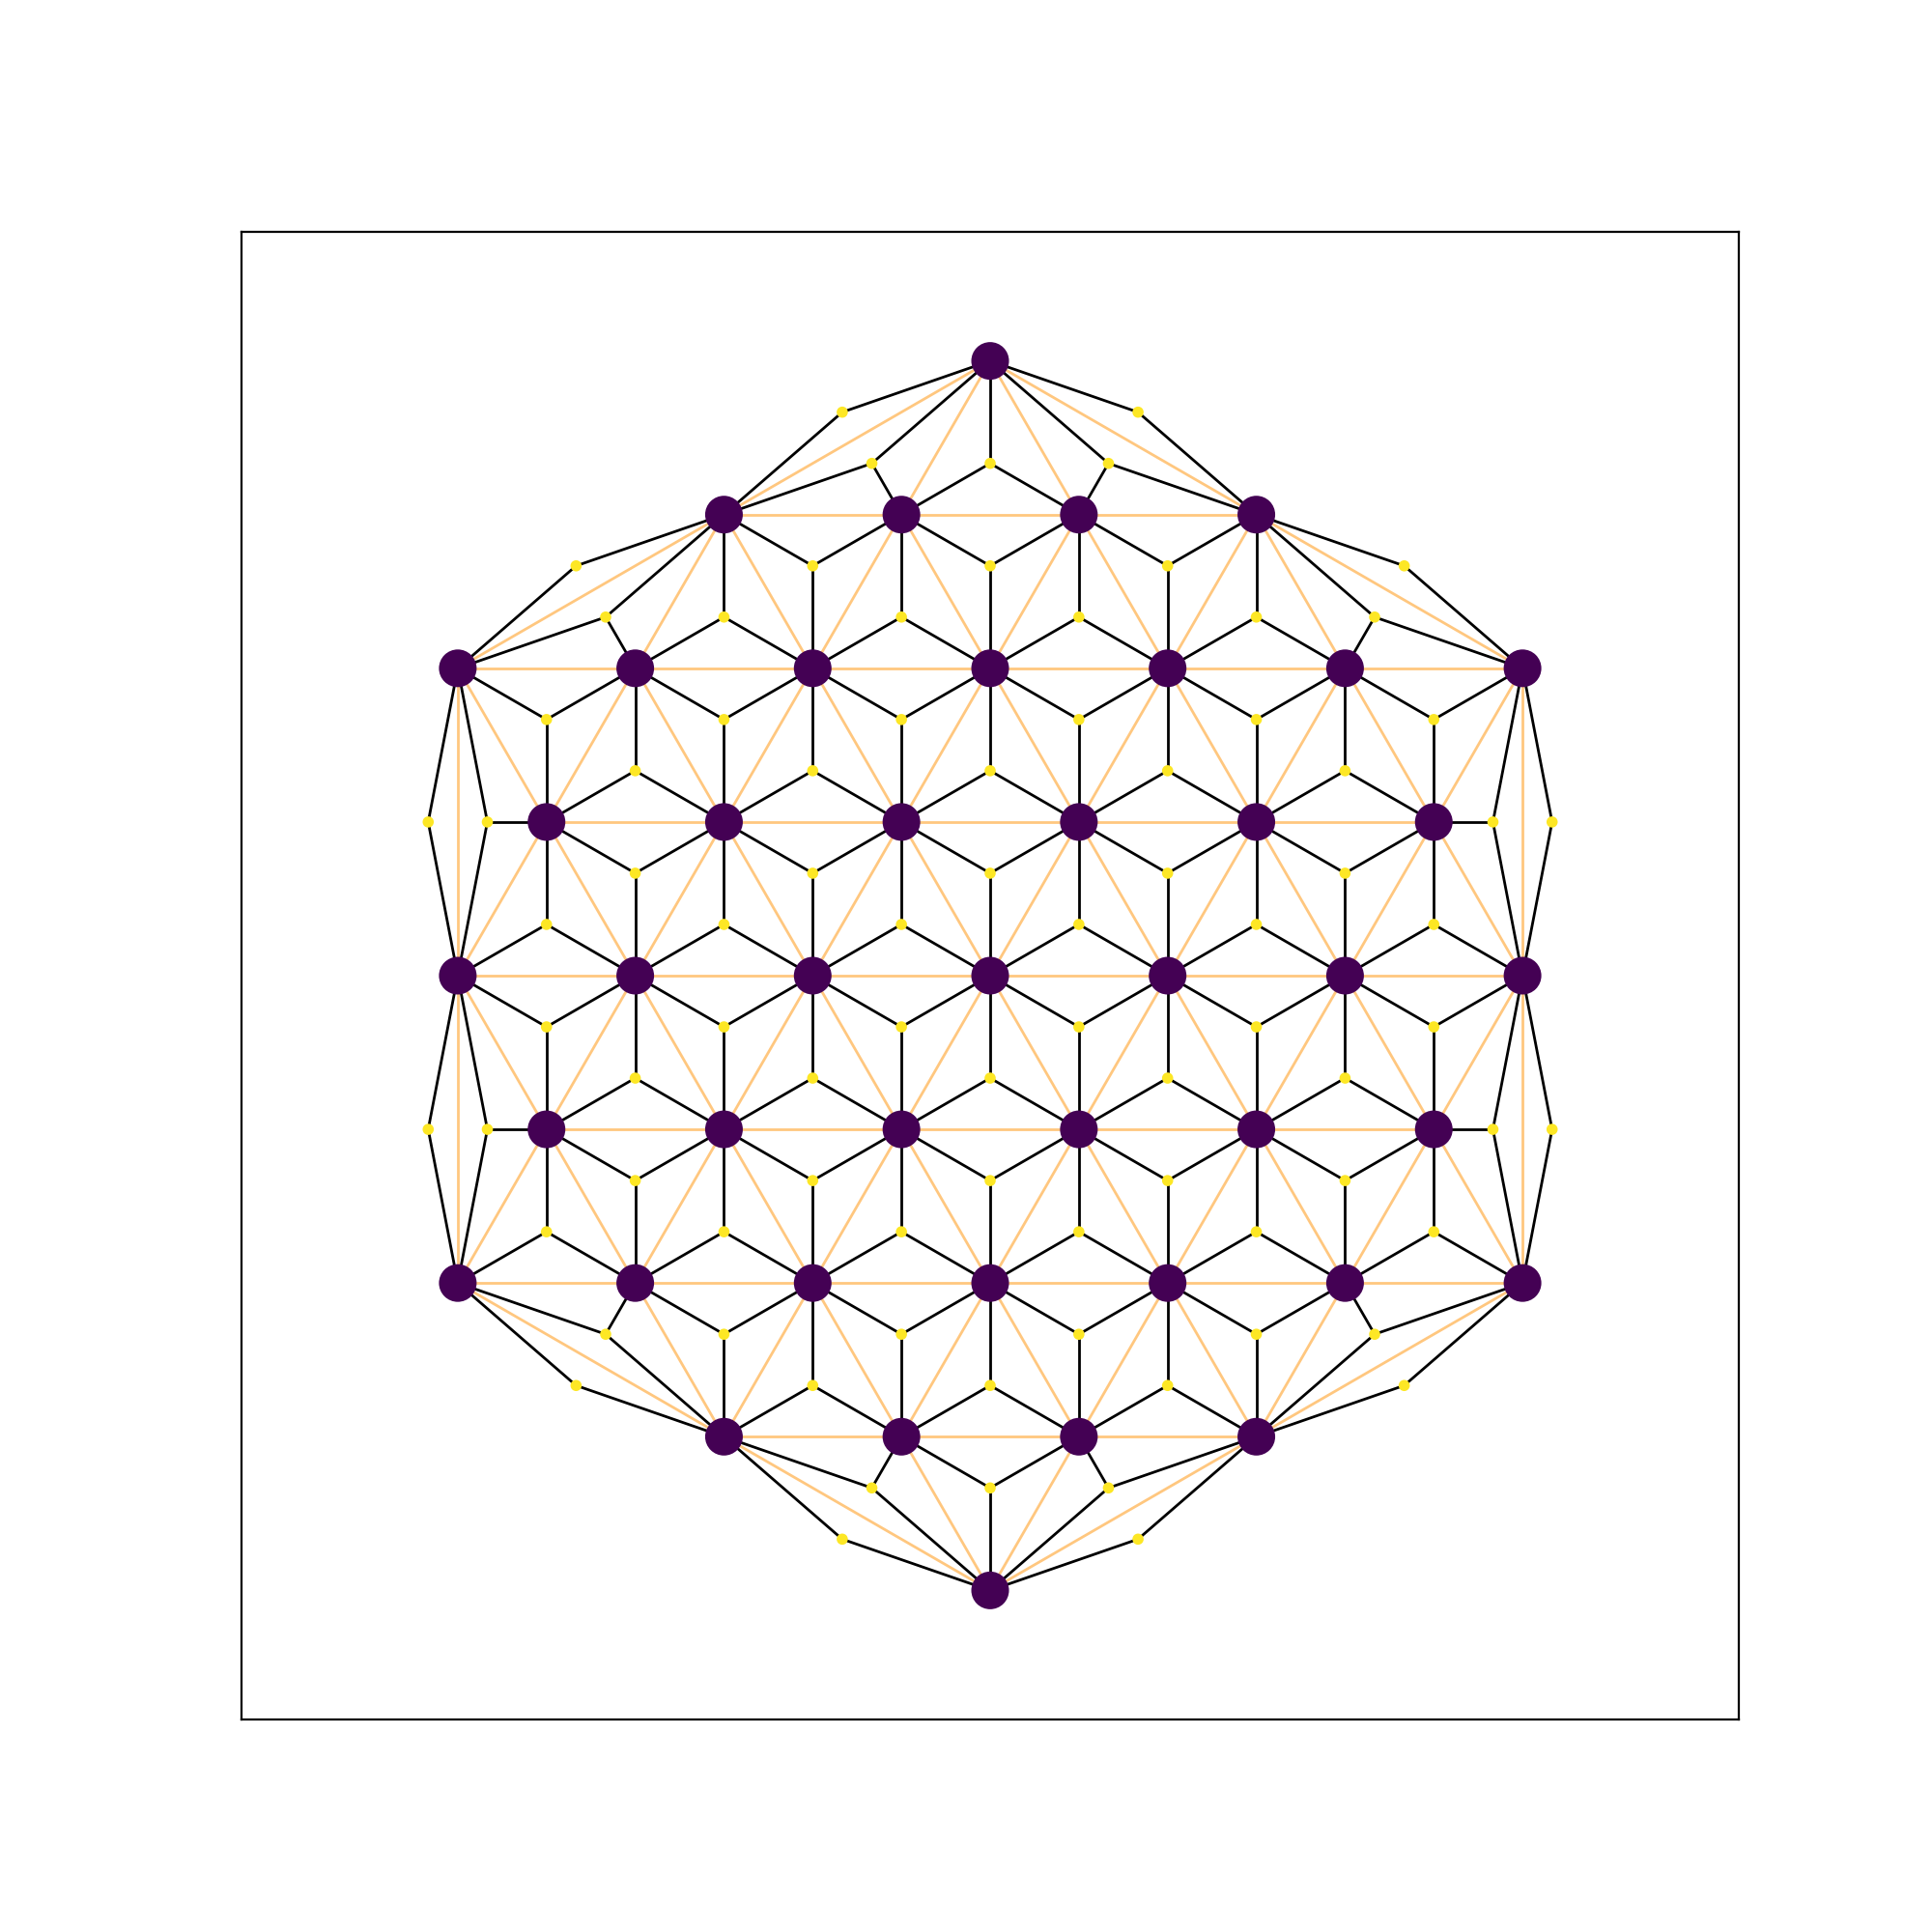
\includegraphics[width=0.5\textwidth]{figures/numerical/hexbig/hexbig_graph.png}
        \caption{Initial lattice drawn as in Figure \ref{fig:layout_init}.}
        \label{subfig:hexbig_graph}
    \end{subfigure}
    \begin{subfigure}[b]{\textwidth}
        \centering
        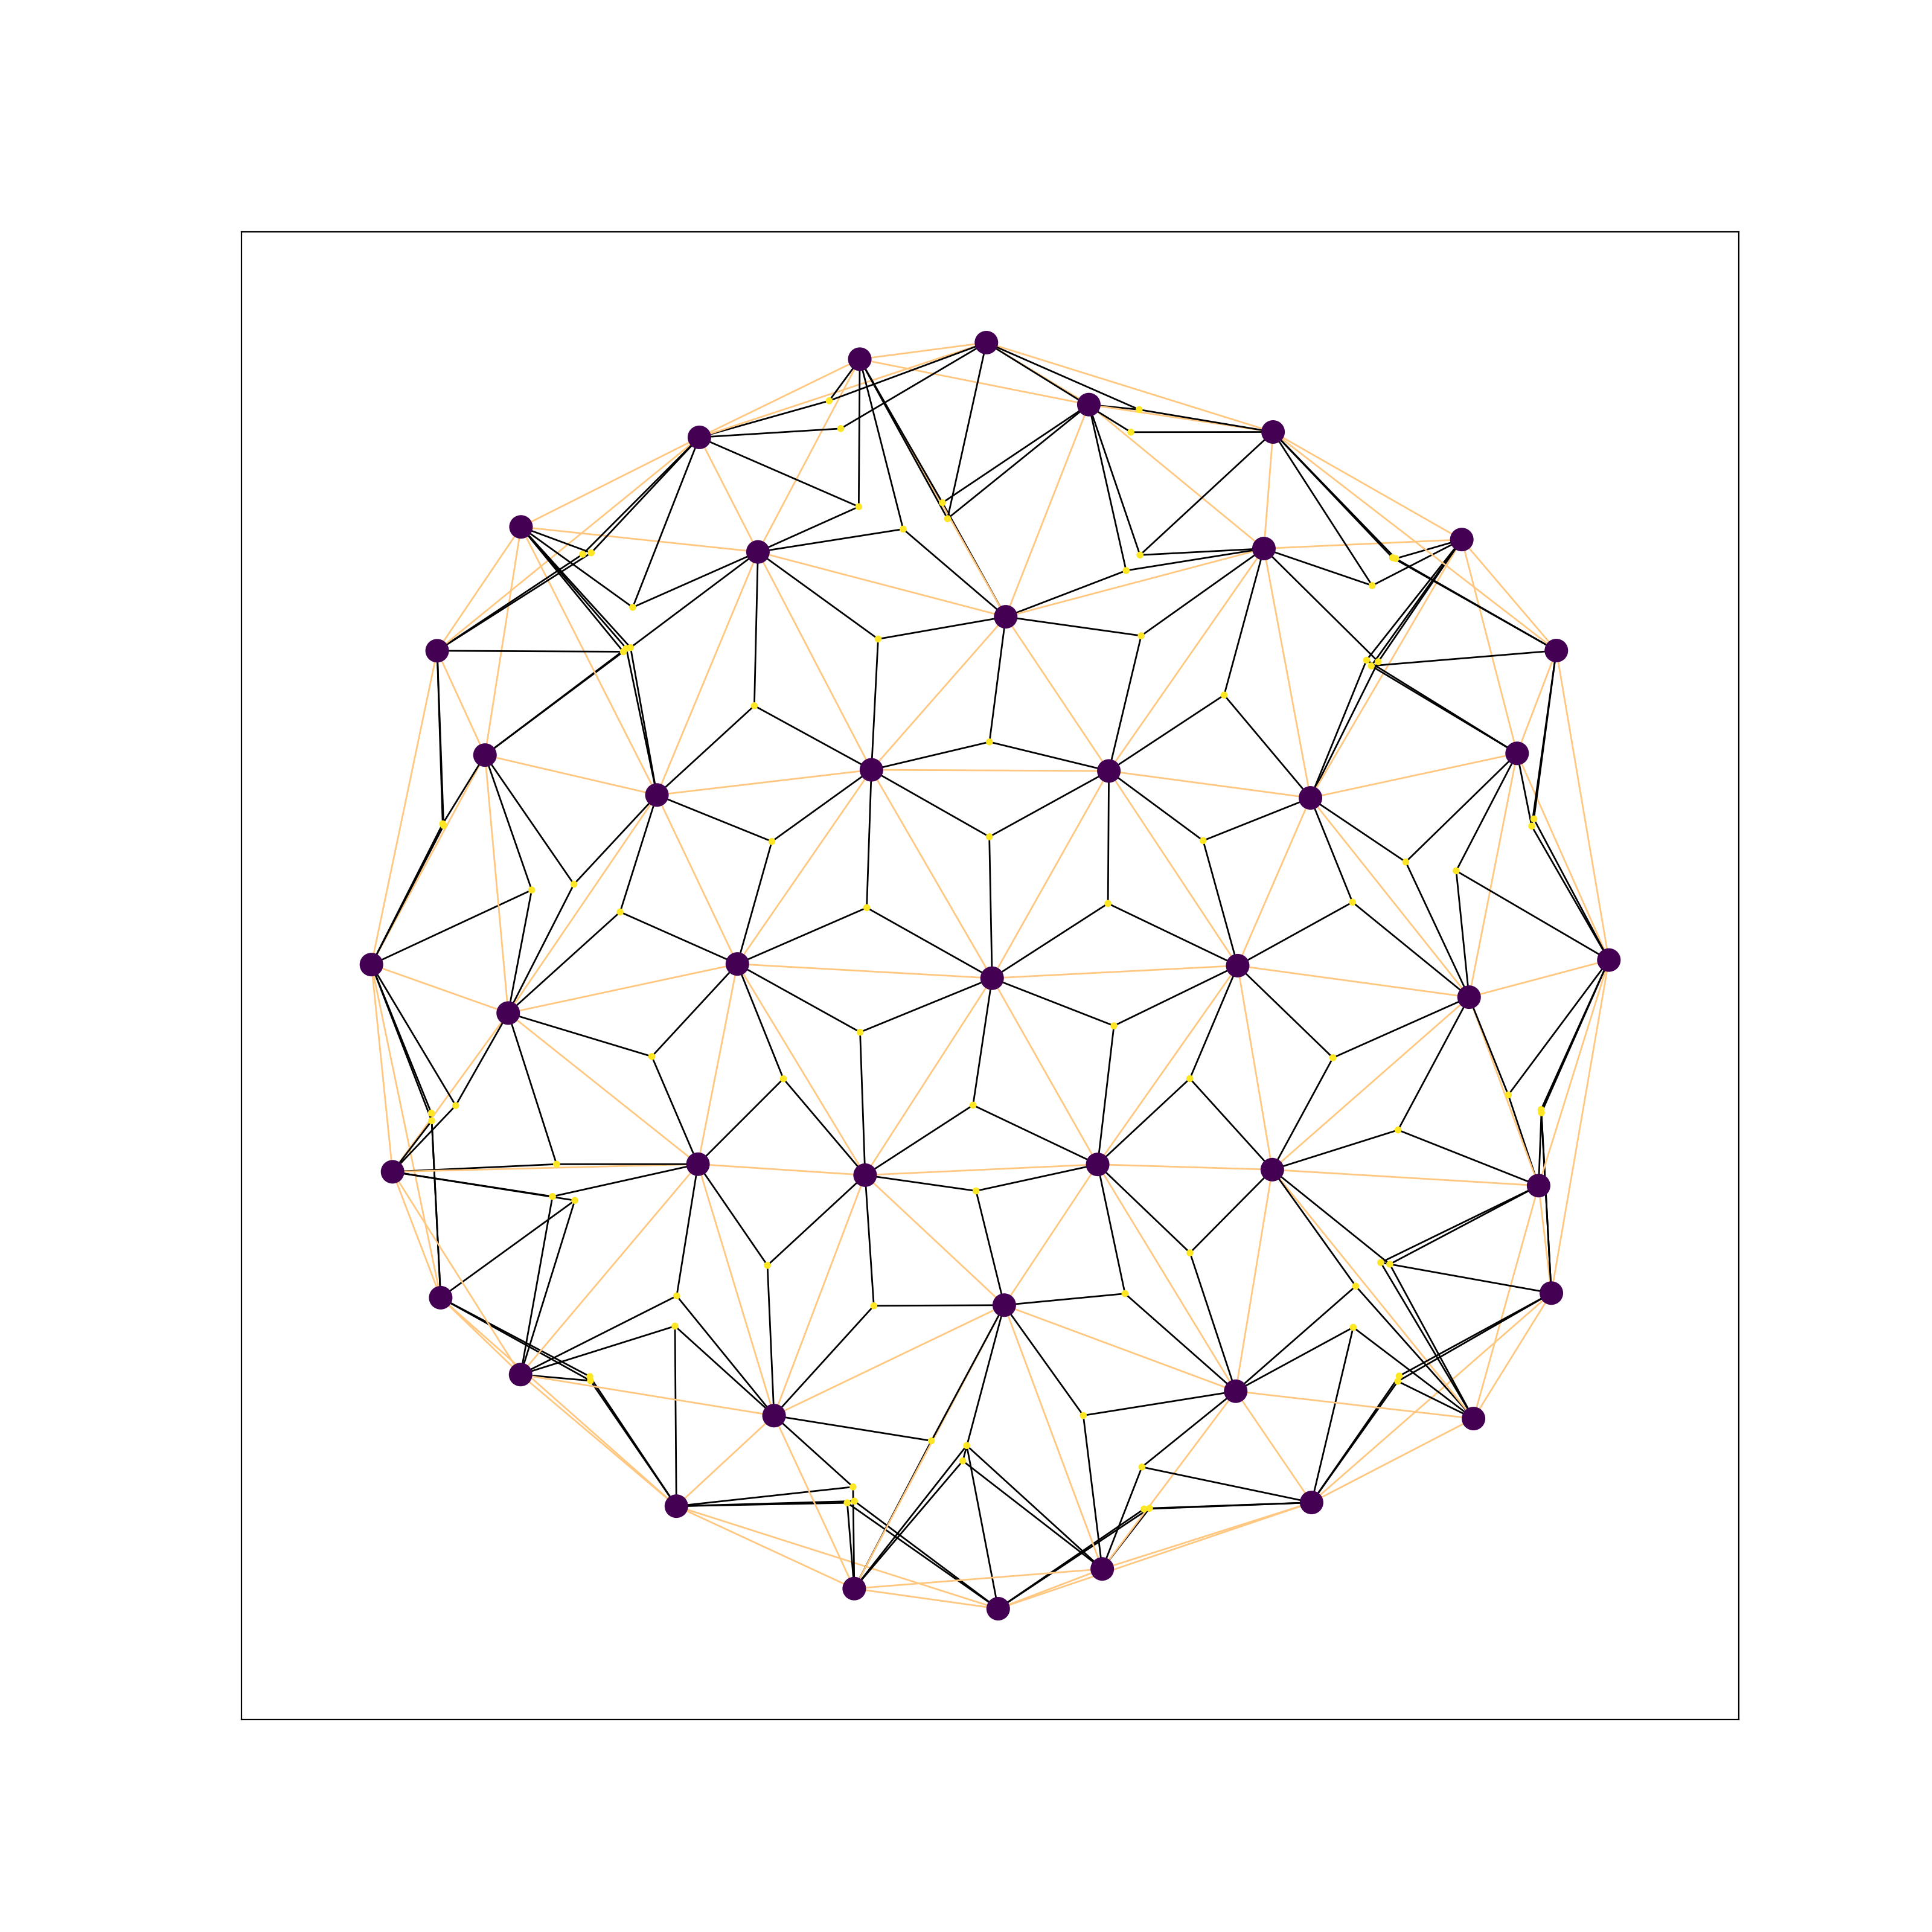
\includegraphics[width=0.3\textwidth]{figures/numerical/hexbig/hexbig0.8_0.8_1.35_10_graph.png}
        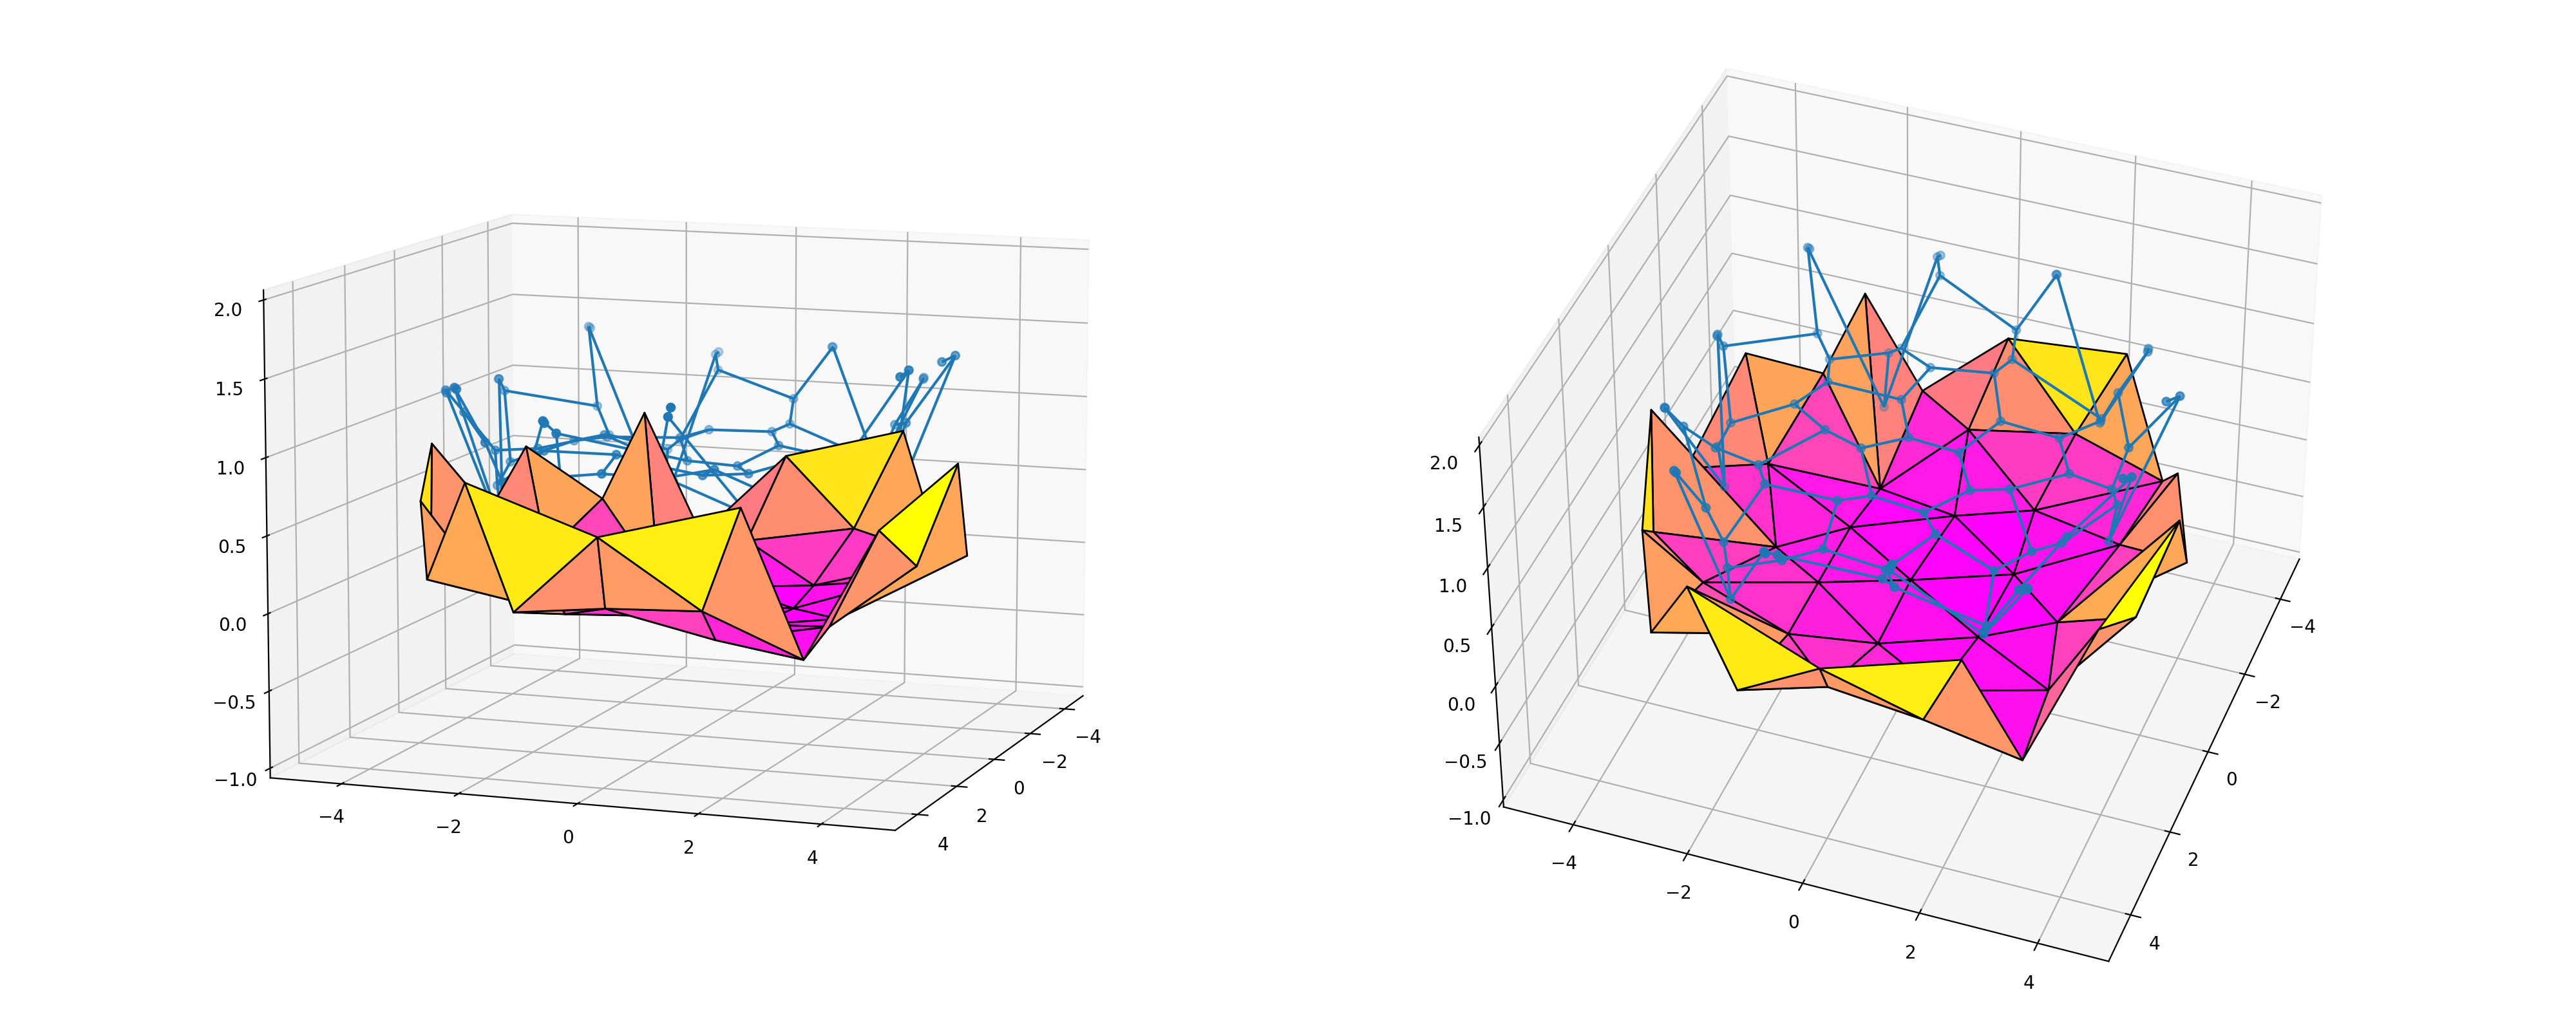
\includegraphics[width=0.69\textwidth]{figures/numerical/hexbig/hexbig0.8_0.8_1.35_10_plot.png}
        \caption{Sheet shape when $\phi_0=0.8$, $\psi_0=0.8$, $\ell_0=1.52$.}
        \label{subfig:hexbig_in}
    \end{subfigure}
    \begin{subfigure}[b]{\textwidth}
        \centering
        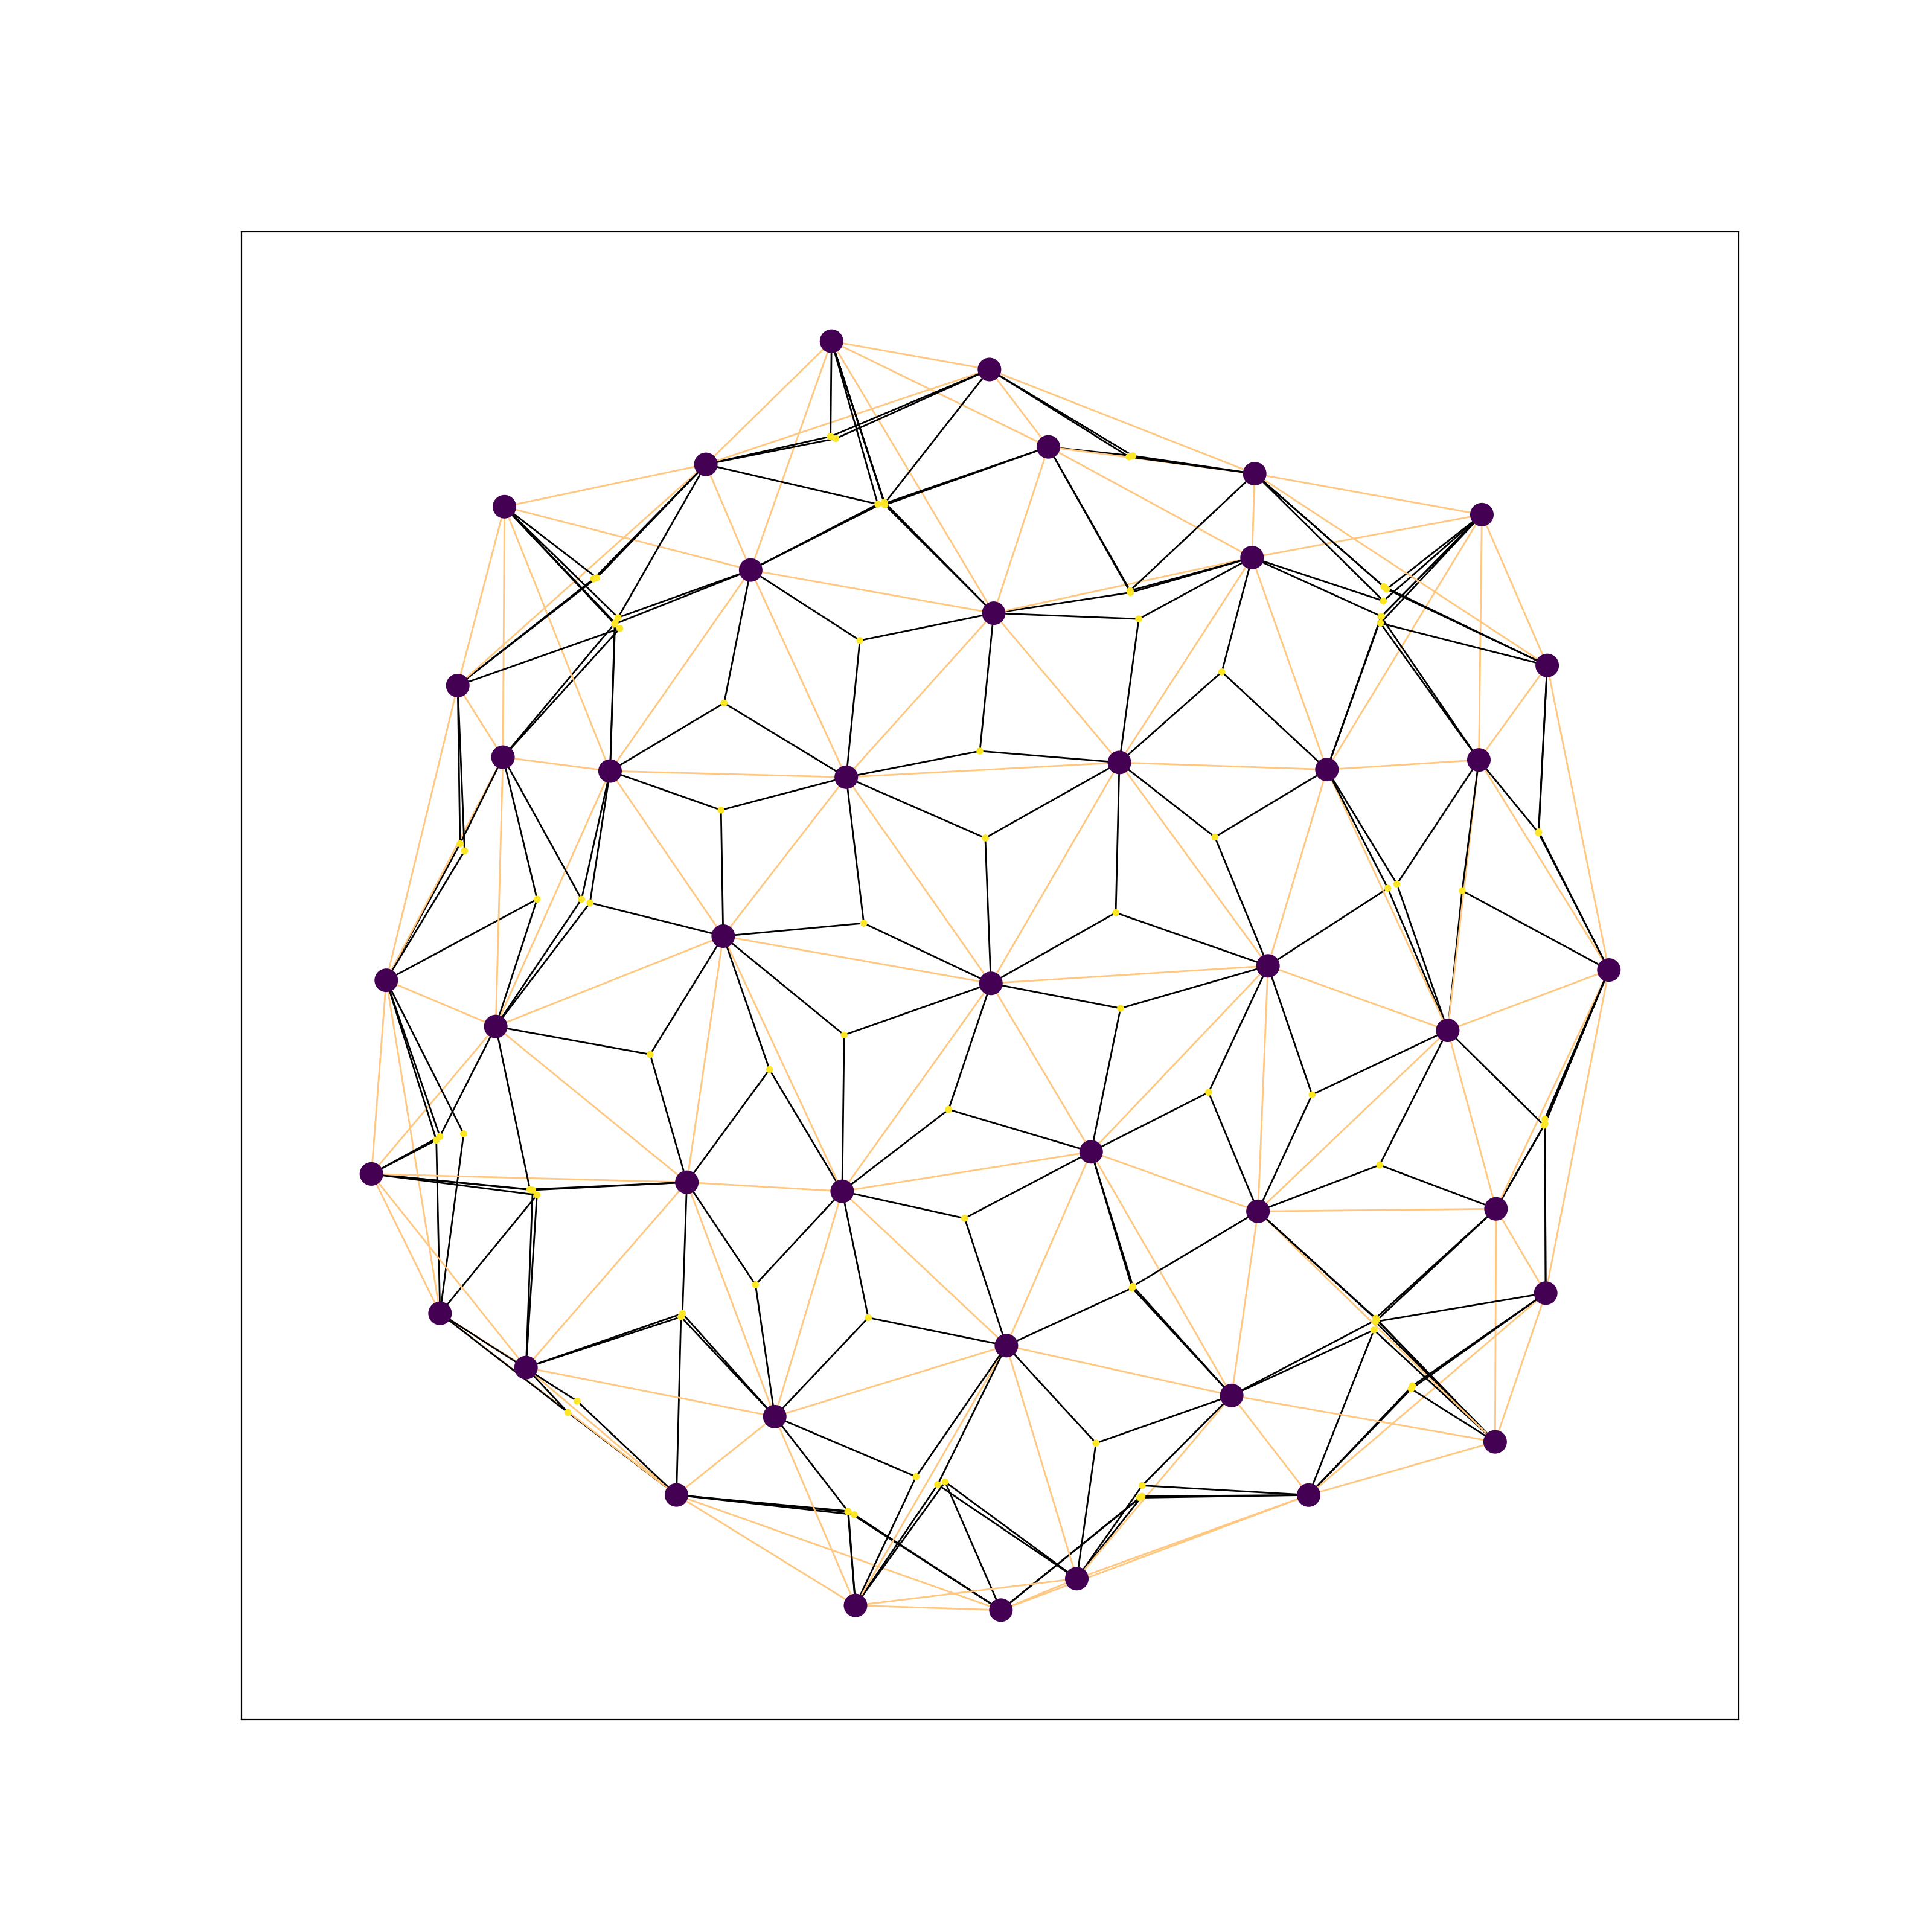
\includegraphics[width=0.3\textwidth]{figures/numerical/hexbig/hexbig0.95_0.8_1.35_10_graph.png}
        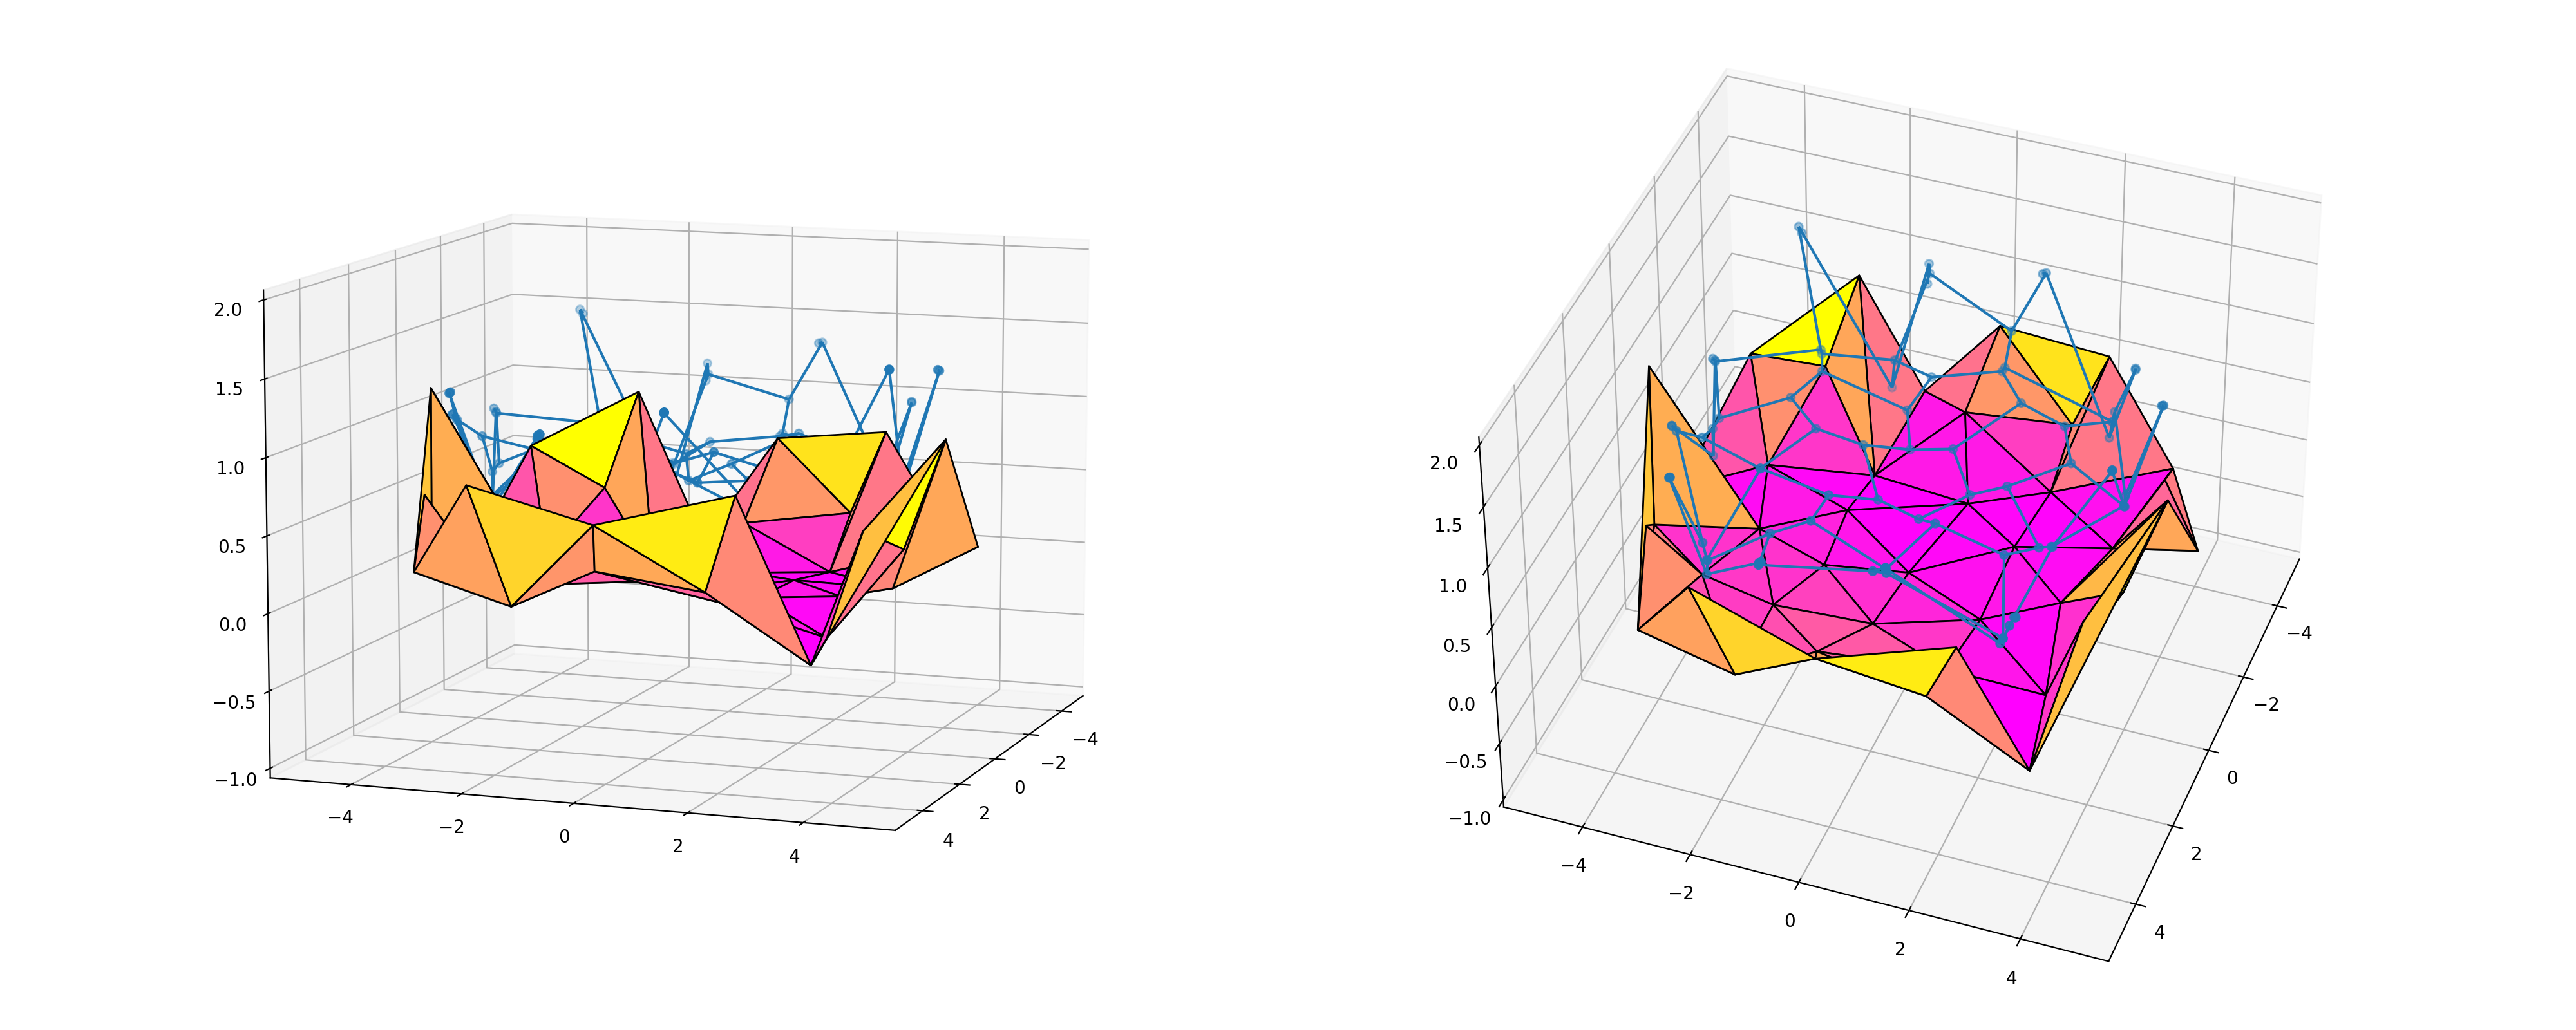
\includegraphics[width=0.69\textwidth]{figures/numerical/hexbig/hexbig0.95_0.8_1.35_10_plot.png}
        \caption{Sheet shape when $\phi_0=0.95$, $\psi_0=0.8$, $\ell_0=1.52$.}
        \label{subfig:hexbig_out}
    \end{subfigure}
    \caption{Cell sheet geometry with a node of degree 7. The graph topology is affected in the sheet interior (subfigure \ref{subfig:hexbig_graph}). This minor change has substantial effects on the sheet geometry (subfigures \ref{subfig:hexbig_in}, \ref{subfig:hexbig_out}).}
    \label{fig:hexbig}
\end{figure}

\section{Varying the energy}

Let the complete energy function $\e[\{r_\gamma, n_\alpha\}]$ be written in terms of sums over the all interactions in the sheet,

\begin{align}
	\e[\{r_\gamma, n_\alpha\}] &= \e_\phi + \e_\psi + \e_{\text{spr}} \\
	&= k_\phi \sum_{(\alpha, \rho)} \left( \phi_{(\alpha, \rho)} - \phi_0 \right)^2 + k_\psi \sum_{(\alpha, \beta: \rho, \sigma)} \left( \psi_{\alpha\beta:\rho\sigma} - \psi_0 \right)^2 + k_{\text{spr}} \sum_{(\alpha, \rho)} \left(\left| \vec{r}_\alpha - \vec{r}_\beta \right| - \ell_0 \right)^2 \label{eq:energy_disc}
\end{align}

\noindent with constants $\phi_0, \psi_0, \ell_0$. We want to find the forces on all relevant points on the sheet by following the gradient of \ref{eq:energy_disc}, 

\begin{align}
	-\vec{F}_\gamma = \frac{\partial \e}{\partial \vec{r}_\gamma} &= 2k_\phi \sum_{(\alpha, \rho)} \left( \phi_{(\alpha,\rho)} - \phi_0 \right) \frac{\partial \phi_{(\alpha,\rho)}}{\partial \vec{r}_\gamma} + 2 k_\psi \sum_{(\alpha, \beta: \sigma, \rho)} \left( \psi_{\alpha\beta:\rho\sigma} - \psi_0 \right) \frac{\partial \psi_{\alpha\beta:\sigma\rho)}}{\partial \vec{r}_\gamma} \nonumber \\
	&\quad + k_{\text{spr}} \sum_{(\alpha, \rho)} \left(\left| \vec{r}_\alpha - \vec{r}_\beta \right| - \ell_0 \right)^2 \label{eq:energy_disc_deriv1} \\
	-\frac{\partial \e}{\partial \bhat{n}_\alpha} &= 2k_\phi \sum_{(\alpha, \rho)} \left( \phi_{(\alpha,\rho)} - \phi_0\right) \frac{\partial \phi_{(\alpha, \rho)}}{\partial \bhat{n}_\alpha}). \label{eq:energy_disc_deriv2}
\end{align}

The gradient described by equations \ref{eq:energy_disc_deriv1} and \ref{eq:energy_disc_deriv2} is solved with derivatives

\begin{align*}
    \frac{\partial \phi_{(\alpha,\rho)}}{\partial r_{\gamma i}} &= \frac{-1}{\sqrt{1 - (\hat{\bm{n}}_\alpha \cdot \hat{(\alpha\rho)})^2}} \left(\frac{\partial \hat{\bm{n}}_{\alpha j}}{\partial r_{\gamma i}} \hat{(\alpha\rho)}_j + \frac{\partial \hat{(\alpha\rho)}_j}{\partial r_{\gamma i}} \hat{\bm{n}}_{\alpha j} \right) \\
    \frac{\partial \hat{(\alpha\rho)}_j}{\partial r_{\gamma i}} &= \frac{(\delta_{\gamma\rho} - \delta_{\gamma\alpha})}{|r_\rho - r_\alpha|} \left( \delta_{ij} + \hat{(\alpha\rho)}_i\hat{(\alpha\rho)}_j \right) \\
    \frac{\partial \psi_{(\alpha, \beta: \sigma, \rho)}}{\partial r_{\gamma i}} &= \frac{-1}{\sqrt{1 - (\hat{\bm{n}}_{\rho\alpha\sigma} \cdot \hat{\bm{n}}_{\rho\beta\sigma}})^2} \left(\frac{\partial \hat{\bm{n}}_{\rho\alpha\sigma j}}{\partial r_{\gamma i}} \hat{\bm{n}}_{\rho\beta\sigma j} + \frac{\partial \hat{\bm{n}}_{\rho\beta\sigma j}}{\partial r_{\gamma i}} \hat{\bm{n}}_{\rho\alpha\sigma j} \right). 
\end{align*}



\begin{align*}	
    \frac{\partial \hat{\bm{n}}_{\alpha j}}{\partial r_{\gamma i}} &= \frac{\mathbb{1}_{\gamma\in \text{collars}(\alpha)} - n\delta_{\gamma\alpha}}{\left| \sum_{(\alpha, \rho)} (r_\rho - r_\alpha) \right|} \left(\delta_{ij} - \hat{\bm{n}}_{\alpha i} \hat{\bm{n}}_{\alpha j} \right) \\
    \frac{\partial \hat{\bm{n}}_{\rho\alpha\sigma j}}{\partial r_{\gamma i}} &= \text{too big see notes}
\end{align*}

\begin{comment}
\newpage
\section{poop}

Typically, membrane mechanics sets $\e = (k_c/2)(2H)^2 = (k_c / 2) (g^{\alpha\beta} K_{\alpha\beta})$. I intend to show that this energy density is also appropriate for a sheet of \textit{C. flexa} if the area formed by each cell's ring of collars is small.



I think there are likely several ways to show this. Note that the second fundamental form $K_{\mu\nu}$ gives an approximation for the height function above the tangent plane at a point: $h\approx K_{\mu\nu}\Delta\xi^\mu\Delta\xi^\nu$ for local chart $\xi^\mu$. Let's assume then that the collar has a fixed length $\ell$ and pivots around a point with preferred angle $\phi_0$. 

Figure \ref{subfig:geom} lays out the geometry for the problem. An equilibrium metric tensor $g_{0\mu\nu}$ and second fundamental form $K_{0\mu\nu}$ correspond to collar angle $\phi_0$, and deforming the membrane results in tensors $g_{\mu\nu}$ and $K_{\mu\nu}$. We can find the difference in angle $\phi_0 - \phi$ by finding the length of the circular arc by which the two states differ when moving from distance $\Delta\vec{\xi}_0$ to $\Delta\vec{\xi}$. 

The setup for finding this arc length $x$ is given in Figure \ref{subfig:arc}. Since we know $K_{\mu\nu}$ approximates the height, we can use ordinary calculus to find the length $x$. Since the change in height $dh$ along a circle is $\ell \cos\theta d\theta$, we know that 

\begin{align}
    K_{\mu\nu}\Delta\xi^\mu \Delta\xi^\nu - K_{0\mu\nu} \Delta\xi_0^\mu \Delta\xi_0^\nu &= \int_{\phi_0}^\phi \ell \cos\phi' d\phi' \nonumber \\
    K_{\mu\nu}\Delta\xi^\mu \Delta\xi^\nu - K_{0\mu\nu} \Delta\xi_0^\mu \Delta\xi_0^\nu &= \ell(\sin\phi - \sin\phi_0) \label{eq:sinphi}
\end{align}

Since we are interested in integrating $(\phi(\theta)-\phi_0)^2$ around the collar, we can take $\Delta\vec{\xi} = r(\cos\theta, \sin\theta)$ to trace a circle from the point of interest on our surface. Here, $r$ is the radius to the collar, and we have unit metric by our choice of coordinates. We are free to take $K_{\mu\nu}$ to be diagonal since it is symmetric (while keeping our basis orthonormal, so our choice of $\Delta\vec{\xi}$ is reasonable). Without making any appoximations besides $h \approx K_{\mu\nu}\Delta\xi^\mu \Delta\xi^\nu$, we return our attention to equation \ref{eq:sinphi}. The radius out from the center to the collar position is $r = \ell \sin \phi$ for $\Delta\vec{\xi}$ and $\ell \sin \phi_0$ for $\Delta\vec{\xi}_0$, so 

\begin{align*}
    \ell^2 \left[K_{11}\sin^2\phi \cos^2\theta - K_{011}\sin^2\phi_0\cos^2\theta + K_{22}\sin^2\phi\sin^2\theta - K_{022}\sin^2\phi_0\sin^2\theta \right] &= \ell(\sin\phi - \sin \phi_0).
\end{align*}

We can assume that the collar filaments all have the same properties, so that $K_{011}=K_{022}=H_0$, which lets us simplify to 

\begin{align}
    \ell^2\left[K_{11}\cos^2\theta + K_{22}\sin^2\theta \right]\sin^2\phi - \ell^2 H_0 \sin^2\phi_0 &= \ell(\sin\phi - \sin\phi_0). \nonumber \\
    \intertext{Dividing out by $\ell$ and rescaling length to take units of $\ell$, we get a relation between the curvature $H_\theta$ in direction $\theta$ and $\sin\phi$: } \nonumber\\
    \underbrace{\left(K_{11}\cos^2\theta + K_{22}\sin^2\theta \right)}_{H_\theta} \sin^2\phi - \sin\phi + \sin\phi_0(1-H_0\sin\phi_0) \nonumber \\
    \sin\phi = \frac{1 \pm \sqrt{1 - 4H_\theta \sin\phi_0(1-H_0\sin\phi_0)}}{2H_\theta}. \label{eq:sinphiequals}
\end{align}

Equation \ref{eq:sinphiequals} 

\begin{align*}
    (K_{\mu\nu} - K_{0\mu\nu}) \Delta\xi^\mu \Delta\xi^\nu &= 2\ell \cos\frac{\phi+\phi_0}{2} \sin\frac{\phi-\phi_0}{2}. \\
    \intertext{Assuming $\phi-\phi_0$ is small, } \\
    (K_{\mu\nu} - K_{0\mu\nu}) \Delta\xi^\mu \Delta\xi^\nu &= \ell \cos\phi_0 (\phi - \phi_0).
\end{align*}


Hence,

\begin{align*}
    \e \sim \ell^2 \cos^2\phi_0 \int_0^{2\pi} (\phi(\theta) - \phi_0)^2d\theta &= \int_0^{2\pi} (K_{\mu\nu} - K_{0\mu\nu})\Delta\xi^\mu \Delta\xi^\nu (K_{\delta\gamma} - K_{0\delta\gamma})\Delta\xi^\delta \Delta\xi^\gamma d\theta \\
    &= r^4\int_0^{2\pi} \left[(K_{11} - K_{011})\cos^2\theta + (K_{22} - K_{022})\sin^2\theta \right]^2 d\theta \\
    \frac{\ell^2 \cos^2\phi_0}{r^4} \int_0^{2\pi} (\phi(\theta) - \phi_0)^2d\theta &= \frac{3\pi}{4} (K_{11} - K_{011})^2 + \frac{2\pi}{4} (K_{11} - K_{011})(K_{22} - K_{022}) + \frac{3\pi}{4}(K_{22} - K_{022})^2 \\
    &= \frac{3\pi}{4} \left[(K_{11} - K_{011})^2 + 2(K_{11} - K_{011})(K_{22} - K_{022}) + (K_{22} - K_{022})^2\right] \\ 
    &\qquad - \pi(K_{11} - K_{011})(K_{22} - K_{022}) \\
    &= \frac{3\pi}{4} \left[\underbrace{(K_{11} - K_{011}) + (K_{22} - K_{022})}_{2(H - H_0)} \right]^2 \\
    &\qquad - \pi \left[ \underbrace{K_{11}K_{22}}_{K} - K_{011}K_{22} - K_{022}K_{11} - K_{011}K_{022}\right].
\end{align*}

Here, we can assume that the collar filaments do not vary around the collar, so $K_{011} = K_{022} = H_0/2$, and we get that

\begin{align}
    \frac{\ell^2 \cos^2\phi_0}{r^4} \int_0^{2\pi} (\phi(\theta) - \phi_0)^2d\theta &= 3\pi (H - H_0)^2 - \pi \left[K + \frac{H_0}{2} (2H) + K_{011}K_{022}\right] \nonumber \\
    \frac{\ell^2 \cos^2\phi_0}{r^4} \int_0^{2\pi} (\phi(\theta) - \phi_0)^2d\theta &= 3\pi(H-H_0)^2 - \pi K - \pi H_0 H - \pi K_{011}K_{022}. \label{eq:angle_energy}
\end{align}

We find that the energy density of our membrane based on angular collar springs has an $(H-H_0)^2$ term and $K$ term. The third right hand side term in equation \ref{eq:angle_energy} can be used to define a different effective curvature $H_0'$ by completing the square with the first, and the last term is a constant contribution to the energy. Since we are interested in varying the energy, we are welcome to discard it.

% Finally we have that $\phi-\phi_0$ is proportional to $K_{\mu\nu} - K_{0\mu\nu}$. Since we are interested in a ring around the point of interest, it is reasonable to take the trace of $K_{\mu\nu}$ to get the mean curvature. This gets us that the energy is proportional to $(2H - H_0)^2$.\footnote{This is handwavy, since I'm integrating then squaring rather than squaring then integrating. }


\subsection{Equation of motion}

When we have the energy density $\e = (k_c/ 2) (2H-H_0)^2$, we could evaluate the divergence of the stress $\nabla_\alpha \bm{F}^\alpha$ or vary the energy functional $E = \int \e(g_{\mu\nu}, K_{\mu\nu}) dS$ directly to get the familiar expression for the force 

\begin{align}
    \bm{f} &= \left[ -k_c (2H + c_0)(2H^2 - c_0H - 2K) - k_c\nabla^2(2H) \right]\hat{\bm{n}}.
\end{align}

When the membrane has a boundary, it is necessary to find the boundary conditions by varying the energy functional directly. The boundary conditions emerge analogously to the process in the Mange representation, and \textcite{tu2003} finds these conditions on boundary $C$ to be 

\begin{align}
    \left[k_c (2H + c_0) \right]_C &= 0 \label{eq:bcs} \\
    \left[-k_c\bm{e}_2\cdot \nabla (2H) \right]_C &= 0 \nonumber \\
    \left[\frac{k_c}{2}(2H + c_0)^2\right]_C &= 0, \nonumber
\end{align}

where $\bm{e}_2$ is the normal vector along the surface perpendicular to $C$. The third boundary condition is clearly redundant with the first when there is no penalty for Gaussian curvature, surface area, or boundary length. As in the Mange representation, the first of these boundary condition equations prescribes a torque-free boundary and the second prescribes force-free.

\subsection{Surface of revolution}

In treating this membrane as a surface of revolution $\bm{r}(\rho, \theta)=(\rho \cos \theta, \rho \sin \theta, z(\rho))$, we can write the mean and Gaussian curvatures in terms of $z$,

\begin{align*}
    H &= \frac{1}{2} \frac{-\rho z'' - z'(1 + z'^2)}{2 \rho (1 + z'^2)^{3/2}} \\
    K &= \frac{z'z''}{\rho (1+z'^2)^2}.
\end{align*}

\textcite{tu2003} chooses to express the resulting ODE by one order by expressing it in terms of the curve's tangent angle $\psi = \arctan{dz/d\rho}$ to get the EOM with boundary conditions

\begin{align}
    \zeta \frac{d\bm{r}}{dt}\cdot\hat{\bm{n}} &= k_c\left(\frac{\sin\psi}{\rho} + \cos \psi \frac{d\psi}{d\rho} - c_0 \right) \left[\frac{1}{2} \left(\frac{\sin\psi}{\rho} + \cos \psi \frac{d\psi}{d\rho} \right)^2 \right. \nonumber \\
    &\qquad \quad \left. + \frac{1}{2} c_0 \left(\frac{\sin\psi}{\rho} + \cos \psi \frac{d\psi}{d\rho} \right) - \frac{2\sin\psi\cos\psi}{\rho} \frac{d\psi}{d\rho} \right] \nonumber \\
    &\quad + k_c \frac{\cos\psi}{\rho}\frac{d}{d\rho} \left[ \rho \cos\psi \frac{d}{d\rho}\left( \frac{\sin\psi}{\rho} + \cos\psi \frac{d\psi}{d\rho} \right) \right] \nonumber \\
    0 &= k_c \left[ \frac{\sin\psi}{\rho} + \cos \psi \frac{d\psi}{d\rho} - c_0 \right]_C \nonumber \\
    0 &= k_c \left[ \cos\psi \frac{d}{d\rho} \left(\frac{\sin\psi}{\rho} + \cos \psi \frac{d\psi}{d\rho} \right) \right]_C. \label{eq:problem}
\end{align}

The second boundary condition is automatically satisfied by the first, however, which specifies that the boundary must have mean curvature $c_0$. Again, this is uniquely the case when the energy density $\e$ only depends on $(2H-c_0)^2$. 

Note that we can nondimensionalise the equation of motion by defining length in units of $1/c_0$ and time in terms of $\zeta / (k_c c_0^2)$. When in equilibrium, the only prescribed constant is $c_0$, which serves to change the length scale of $\rho$. What we get as a result is that there is only one shape resulting from equations \ref{eq:problem} that is rescaled according to $c_0$. 

\subsection{Numerical solution}

\textcite{tu2010} shows that the equilibrium shape equation can be reduced to

\begin{align}
    \ddot{\psi} &= -\frac{\psi}{2} \dot{\psi}^2 - \frac{\cos\psi \dot{\psi}}{\rho} + \frac{\sin2\psi}{2\rho^2} + \frac{\tan\psi}{2}\left(\frac{\sin\psi}{\rho} - c_0 \right)^2 \label{eq:lower_order}
\end{align}

\noindent where the dot indicates derivation with respect to arc length. I forward integrated equation \ref{eq:lower_order} to find the equilibrium shape of a membrane with prescribed $c_0$, and evaluated the mean curvature (the boundary condition in equation \ref{eq:problem}) to find where the curve ends. Integrating equation \ref{eq:lower_order} gives the shape in Figure \ref{subfig:shape_untrimmed}. Evaluating the boundary condition provides a final shape with that wraps around, as shown in Figure \ref{subfig:shape}.

\begin{figure}[tbp]
    \centering
    \begin{subfigure}[b]{0.48\textwidth}
        \centering
        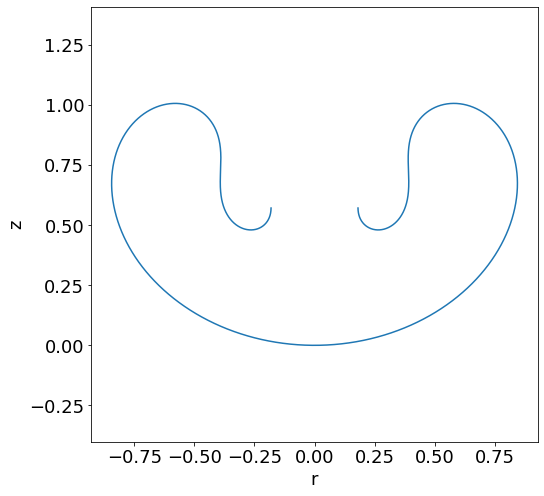
\includegraphics[width=\textwidth]{figures/shape.png}
        \caption{Curve resulting from integrating equation \ref{eq:lower_order}.}
        \label{subfig:shape_untrimmed}
    \end{subfigure}
    ~
    \begin{subfigure}[b]{0.48\textwidth}
        \centering
        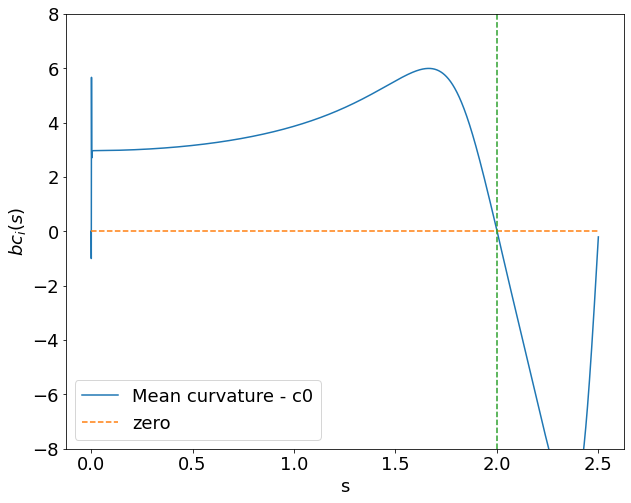
\includegraphics[width=\textwidth]{figures/bcs.png}
        \caption{The evaluation of the boundary condition from equations \ref{eq:problem} in the shape shown in \ref{subfig:shape_untrimmed}.}
        \label{subfig:bcs}
    \end{subfigure}
    \\
    \begin{subfigure}[b]{0.48\textwidth}
        \centering
        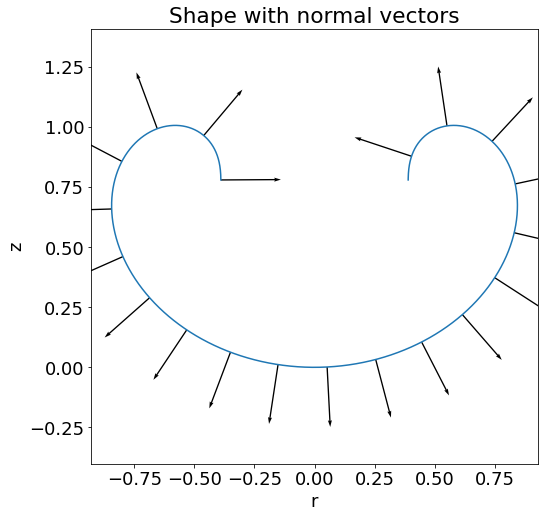
\includegraphics[width=\textwidth]{figures/normals.png}
        \caption{Curve from \ref{subfig:shape_untrimmed} trimmed to satisfy torque- and force-free boundary conditions based on \ref{subfig:bcs}. Unit normal vectors are shown.}
        \label{subfig:shape}
    \end{subfigure}
    \caption{Shape resulting from solving problem \ref{eq:problem}.}
    \label{fig:shape}
\end{figure}

Immediately after integrating, $\psi$ is easily expressed as a function of arclength $s$, since $s$ is proportional to the number of integration steps. \textcite{tu2003} expresses equation \ref{eq:problem} in terms of $\psi(s)$

\begin{align}
    \zeta \frac{d\bm{r}}{dt} \cdot \hat{\bm{n}} &= (2-3\sin^2\psi)\dot{\psi}\rho - \sin\psi (1 + \cos^2\psi) + \left[c_0^2\dot{\psi} - \dot{\psi}^3 - 2\overset{\cdots}{\psi} \right]\rho^3 \nonumber \\
    &\quad+ \left[c_0^2 \sin\psi - 4 c_0 \sin\psi \dot{\psi} + 3\sin\psi (\dot{\psi})^2 - 4 \cos\psi \ddot{\psi} \right]\rho^2 . \label{eq:problem_s}
\end{align}

At the instant that $c_0 \to -c_0$, only one term in the above force changes. Since we know that the right hand side (with $+c_0$) is equal to zero, we can subtract it to know that the force at $t=0$ is exactly 

\begin{align}
    \bm{f}(t=0)= \zeta \frac{d\bm{r}}{dt} \cdot \hat{\bm{n}} &= -8 c_0 \sin\psi \dot{\psi} \rho^2. \label{eq:force_exact}
\end{align}

The force as calculated numerically by equation \ref{eq:problem_s} is shown in Figure \ref{fig:force}.

\begin{figure}[htbp]
    \centering
    \begin{subfigure}[b]{0.48\textwidth}
        \centering
        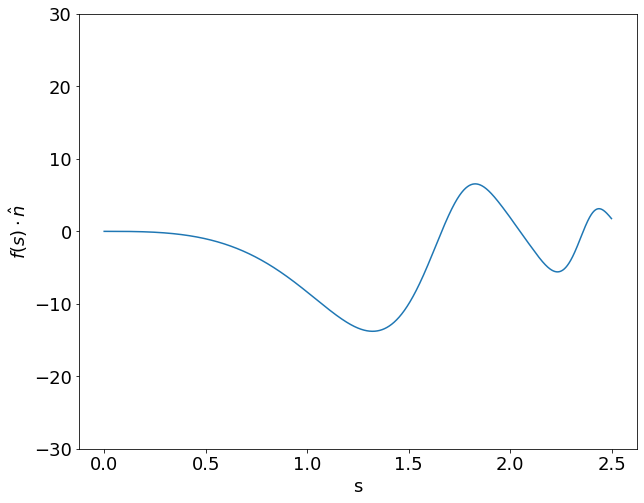
\includegraphics[width=\textwidth]{figures/force.png}
        \caption{Force on the membrane as a function of arclength from the center along a meridian, calculated numerically with equation \ref{eq:problem_s}. Evaluated at $t=0$, the instant that $c_0 \to -c_0$, on the equilibrium shape}
        \label{subfig:force}
    \end{subfigure}
    ~
    \begin{subfigure}[b]{0.48\textwidth}
        \centering
        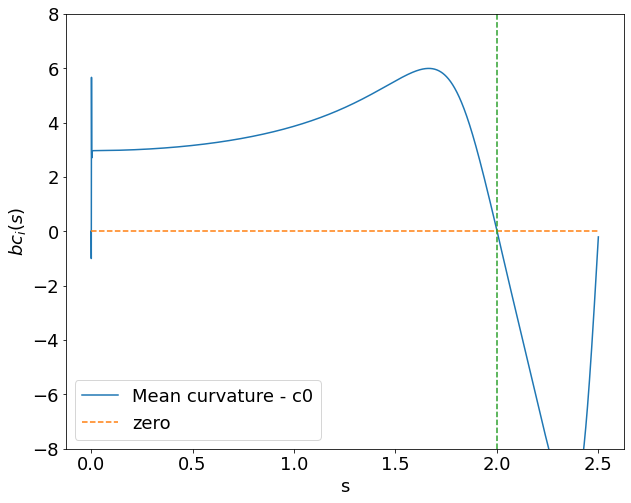
\includegraphics[width=\textwidth]{figures/bcs.png}
        \caption{The force shown in \ref{subfig:force} overlaid on the $t=0$ membrane shape from Figure \ref{fig:shape}.}
        \label{subfig:deform}
    \end{subfigure}
    \caption{Forces acting on the membrane at $t=0$.}
    \label{fig:force}
\end{figure}

We are able to avoid numerical issues in solving problem \ref{eq:problem} at $t=0$ because we know that we are using the equilibrium shape. In other words, even though we used equation \ref{eq:lower_order} to find the shape and equation \ref{eq:problem_s} to find the force, we can use the trick in equation \ref{eq:force_exact} to cancel out any numerical issues arising from integration. Since equation \ref{eq:problem_s} has a third derivative, small bumps in $\ddot{\psi}$ are magnified, but they can be canceled by what we know to be analytically (but not numerically) equal to zero. Figure \ref{fig:instability} shows what the force looks like without subtracting the evaluation of equation \ref{eq:problem_s} for $c_0$.

\begin{figure}[]
    \centering
    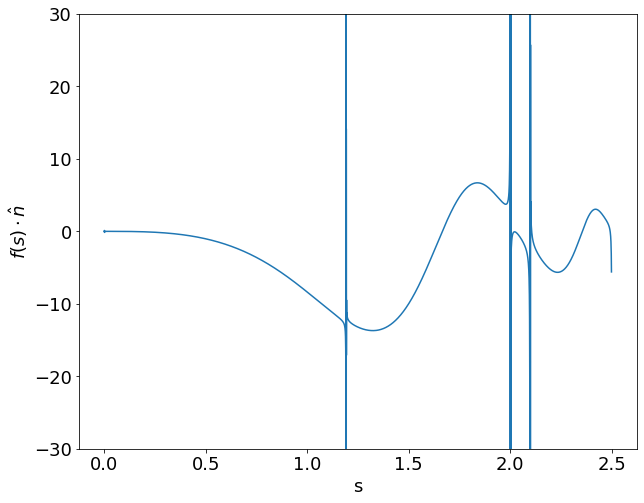
\includegraphics[width=0.6\textwidth]{figures/instability.png}
    \caption{The force as shown in Figure \ref{fig:force} with numerical issue included.}
    \label{fig:instability}
\end{figure}

Regardless of how we resolve numerical issues at $t=0$, we know that we are able to resolve them because we know analytically that the shape equation equals zero then. However, we run into two issues the moment we begin to simulate dynamics in time.

\begin{enumerate}
    \item We no longer know that some expression is exactly zero, so we must resolve the issues purely numerically.
    \item The discrete points of our curve are no longer spaced with equal intervals, so we can't use arclength as our parameterisation anymore. We will need to use \ref{eq:problem}, which will have numerical issues as well due to the $\frac{d}{d\rho}$s. Any place where $\psi = \pi/2$ will become an issue.
\end{enumerate}

\end{comment}

\printbibliography

\end{document}
